\documentclass[12pt]{article}

\usepackage[english]{babel}
\usepackage[utf8x]{inputenc}
\usepackage{amsmath}
\usepackage{graphicx}
\usepackage{longtable}
\usepackage{hyperref}
\usepackage{natbib}
\usepackage{deluxetable}

\newcommand\tbd[1]{\textbf{\color{red}(#1)}}

\newcommand\x         {\hbox{$\times$}}
\newcommand\othername {\hbox{$\dots$}}
\def\eq#1{\begin{equation} #1 \end{equation}}
\def\eqarray#1{\begin{eqnarray} #1 \end{eqnarray}}
\def\eqarraylet#1{\begin{mathletters}\begin{eqnarray} #1
                  \end{eqnarray}\end{mathletters}}
\def\mic              {\hbox{$\mu{\rm m}$}}
\def\about            {\hbox{$\sim$}}
\def\Mo               {\hbox{$M_{\odot}$}}
\def\Lo               {\hbox{$L_{\odot}$}}
\def\comm#1           {{\tt (COMMENT: #1)}}
\def\kms   {\hbox{km s$^{-1}$}}
\def\email#1{\href{mailto:#1}{\nolinkurl{#1}}}

% Journal definitions for bibtex:
\def\jnl#1{{\it#1\/}}
\def\apj{\jnl{ApJ}}
\def\apjl{\jnl{ApJL}}
\def\apjs{\jnl{ApJS}}
\def\aj{\jnl{AJ}}
\def\apss{\jnl{Ap\&SS}}
\def\mnras{\jnl{MNRAS}}
\def\aap{\jnl{A\&A}}
\def\aaps{\jnl{A\&AS}}
\def\nat{\jnl{Nature}}
\def\physrep{\jnl{Phys. Rep.}}
\def\araa{\jnl{ARAA}}
\def\prd{\jnl{Phys.\ Rev.\ D}}
\def\pasp{\jnl{PASP}}
\def\pasj{\jnl{PASJ}}
\def\pasa{\jnl{PASA}}
\def\aaps{\jnl{A\&AS}}
\def\an{\jnl{AN}}
\def\jcap{\jnl{JCAP}}
\def\memsai{\jnl{Mem. Soc. Astron. Ital.}}
\def\icarus{\jnl{Icarus}}
\def\planss{\jnl{Planet.~Space~Sci.}}

\usepackage[usenames]{color}
\newcommand{\G}[1]{{\color{red} #1}}
\newcommand{\B}[1]{{#1}}
\newcommand{\R}[1]{{\color{red}}}

% \code{...} sets code in \tt and escapes most special characters.  Doesn't
% handle {} correctly, but \CODE.anything but period. does (actually, you
% may use any character as a delimiter).
% Designed for a word or two of code inline; use
% \begin{verbatim}...\end{verbatim} for longer blocks
\def\uncatcodespecials{\def\do##1{\catcode`##1=12}\dospecials}%
{\catcode`\`=\active\gdef`{\relax\lq}}% this line inhibits Spanish ligatures ?` and !` of \tt font
\def\setupcode % see TeX Book, p. 381
    {\tt %
     \spaceskip=0pt \xspaceskip=0pt % just in case...
     \catcode`\`=\active
     \uncatcodespecials \obeyspaces
     \catcode`\{=1\catcode`\}=2
    }%
\def\SETUPCODE % see TeX Book, p. 381
    {\tt %
     \spaceskip=0pt \xspaceskip=0pt % just in case...
     \catcode`\`=\active
     \uncatcodespecials \obeyspaces
    }%
\def\docode#1{#1\endgroup}%
\def\DOCODE#1{\def\next##1#1{##1\endgroup}\next}%
\def\code{\begingroup\setupcode\docode}%
\def\CODE{\begingroup\SETUPCODE\DOCODE}%


\title{Hyper Suprime-Cam Survey \\
  Pipeline Description}
\author{
  The HSC Pipeline Team: \\ \\
  Hisanori Furusawa,
  Michitaro Koike,
  Yuki Okura, \\
  Tadafumi Takata,
  Yoshihiko Yamada, \\
  Hitomi Yamanoi (NAOJ Mitaka) \and
  Naoki Yasuda,
  Steven Bickerton, \\
  Nobu Katayama,
  Sogo Mineo (IPMU) \and
  Robert Lupton,
  Jim Bosch,
  Craig Loomis, \\
  Hironao Miyatake,
  Paul Price,
  Kendrick Smith (Princeton) \and
  Dustin Lang (CMU) \\
}


\begin{document}
\maketitle
\pagestyle{headings}

\begin{abstract}
This document describes the Hyper Suprime-Cam Survey Pipeline, which
will be used to process observations obtained as part of the HSC Survey,
and release the processed images and catalogs to the survey collaboration, and
ultimately the world.  The pipeline team hopes that this document will
be of use to survey collaboration members evaluating the pipeline and its
products for their use in science programs.
\end{abstract}

\clearpage

\tableofcontents

\clearpage

\section{Introduction}

This document describes the Hyper Suprime-Cam (HSC) Survey Pipeline, which will be used to process the survey
observations and deliver data products with a consistent high quality to the collaboration, and ultimately to
the world, for the realization of the survey science goals.

\subsection{Hyper Suprime-Cam}

%%%
%%% Stolen from the SSP proposal, with some edits
%%%

HSC takes advantage of the full accessible field of view of the Subaru telescope (1.5~deg diameter).  The
focal plane is paved with 104 Hamamatsu Deep Depletion science CCDs (plus another 12 guiding and focus CCDs),
each 2k\x 4k, with four independent readout amplifiers.  The same CCDs are currently installed
in Suprime-Cam, which has demonstrated their excellent characteristics: low read noise, excellent charge
transfer efficiency, few cosmetic defects, and most importantly, high quantum efficiency from 4000\AA\ to
10,000\AA.  The CCD pixels are $15\mu$m on a side, corresponding to $0.168$~arcsec at the focal plane. At this
resolution, the images will be well-sampled in even the best seeing.  Ray-tracing of the optics has shown that
ghosting is minimal, with the worst ghost at an illuminance (fractional light in a PSF aperture) of $\sim 5
\times 10^{-8}$.

Details of the instrument are summarized in the HSC Design Review
Booklet\footnote{\url{http://anela.mtk.nao.ac.jp/hypersuprime/presentation/hscreview20090227final_combined.pdf}}. The
official HSC web page\footnote{\url{http://www.naoj.org/Projects/HSC/index.html}} provides up-to-date
information.

\subsection{The HSC Survey}

%%%
%%% Stolen from the SSP proposal, with edits
%%%

The HSC Survey was initiated to address key scientific questions using the new capabilities afforded by HSC.
The principal science drivers are:
\begin{itemize}
\item Studies of the properties of dark matter and dark energy as a
  function of redshift, using measurements of galaxy clustering, weak
  lensing, supernovae, cross-correlation with high-resolution maps
  of the Cosmic Microwave Background, and studies of high-redshift
  quasars.
\item Studies of the evolution of galaxies over cosmic time, with
  emphasis on stellar populations and star formation, morphologies, and
  active nuclei.
\end{itemize}

The survey has a classical ``wedding cake'' design, with three layers.  The Wide layer will cover roughly
1,400~deg$^2$ in five broad filters ($grizy$), with exposure times of $10-20$~min per pointing (and one with a
shorter exposure time of $\sim 30$~sec to enable astrometric and photometric calibration with other surveys).
This will go to a point-source depth of $r\sim 26$, and is optimized for weak-lensing science.  Using galaxies
for weak lensing will require exquisite understanding of their properties and evolution, which will be the
motivation of the Deep layer, covering 27~deg$^2$ in four distinct fields, going roughly one magnitude deeper
with exposures of roughly 1~hr per filter.  In addition to the broad-band filters, the Deep layer will include
imaging in three narrow-band filters, to detect Lyman-$\alpha$ emitters and study their luminosity function
and clustering properties at $z = 2.2$, 5.7, and 6.6.

To study the faintest and most distant galaxies, and to probe the
transient universe, especially high-redshift supernovae, will require
the Ultradeep layer, going another magnitude fainter yet.  Narrow-band
filters in the Ultradeep layer will search for Lyman-$\alpha$
emitters at $z = 5.7$, 6.6, and 7.3 at the very faint end of the
luminosity function.

More information about the HSC Survey is available from the Strategic Survey Program
proposal\footnote{\url{http://hscsurvey.pbworks.com/Draft-Strategic-Survey-Proposal}} and the HSC Survey White
Paper\footnote{\url{http://hscsurvey.pbworks.com/HSC_Science_White_Paper}}.

\subsection{This document}

This document provides a reference to the HSC Survey Pipeline, which will be
used to process the HSC Survey observations, producing the necessary
data to achieve the scientific goals of the survey.  It is
especially intended for HSC Survey scientists to evaluate the pipeline
and its products in relation to their own science goals.

In section \ref{sec:pipeline}, we outline the pipeline construction and operations, tracing the flow of data
through the various stages of the pipeline, to the ultimate releases to the collaboration.  Next, in section
\ref{sec:products}, we outline the various products that will compose the data releases, with particular
attention to the measurements that comprise the catalog in the database.  Section \ref{sec:algorithms} gives
details as to the algorithms used to make these measurements, and section \ref{sec:access} describes how
the data will be made available.  Finally, section \ref{sec:support} contains pointers on resources available
for supporting users of these data.


\section{The HSC Pipeline}
\label{sec:pipeline}
\subsection{Software}

%%%
%%% Stolen from the SSP proposal
%%%

To construct the HSC pipeline, we use the LSST pipeline software\footnote{\url{http://dev.lsstcorp.org}}
as the foundation.  This is a synergistic
effort, since the pipelines have similar functionality.  By this scheme, the HSC pipeline has features and a
maturity it would not otherwise have at this stage, and because our pipeline is based on code with a larger
market share than ours could ever have alone, we can have greater confidence in the results.  In return, LSST
gains testing and verification with real-world data.  However, since LSST is a larger-scale development
project not entirely within our control, we are selective about the LSST components we use for the HSC
pipeline, so that we are not chained to every design decision of LSST.  We have also supplemented LSST
components with different algorithms, and added new pipeline components as necessary.  The LSST code is
released under the GNU Public License, version 3 (or later), and our releases of our modified versions of that
code, and our own code (as a ``derivative work'') are bound to use the same license.

The pipeline is written in Python, using C++ for low-level algorithmic components where speed is important.
SWIG is used to wrap the C++ components so they can be called directly from Python.  The combination of these
results in all the ease and flexibility of a scripting language while retaining the power of a compiled
language.

Particular attention has been paid, in large part because of our contributions, to making the LSST pipeline
extensible and configurable.  New camera interfaces and new measurement algorithms can be added without the
need to redesign or even rebuild the software.  The modular design also allows for algorithms to be
substituted at run-time, so that the pipeline can be adapted to the data being processed.
These features, besides
being useful for our adaptation of the LSST pipeline to HSC, mean that we could use our own pipeline to
process data from other telescopes and cameras for comparison with the results of other pipelines (e.g., we
can not only compare the results of the HSC Survey + HSC pipeline with DECam + DES pipeline, but also with
DECam + HSC pipeline, for better diagnosis of any problems).  Interface packages have been written for LSST
simulated images (``ImSim''), CFHT MegaCam, Subaru's Suprime-Cam and HSC, SDSS, and DECam.

Testing with archival Suprime-Cam data (in particular, from after August 2008 when the Hamamatsu CCDs were
installed) and more recently with HSC commissioning data has been an integral part of the pipeline development.

\subsection{Data flow}

The pipeline consists of multiple stages in order to produce the variety of data products required to meet the
various survey science goals.  The stages share a great deal of framework code, but differ by their inputs,
parallelism scheme (CCD vs exposure vs sky patch) and outputs.  Different science applications will depend on
different pipeline stages, according to the desired measurements, depth and accuracy.  Understanding the data
flow is key to matching science goals with the various measurements provided by the pipeline.

\begin{figure}[!htbp]
    \centering
    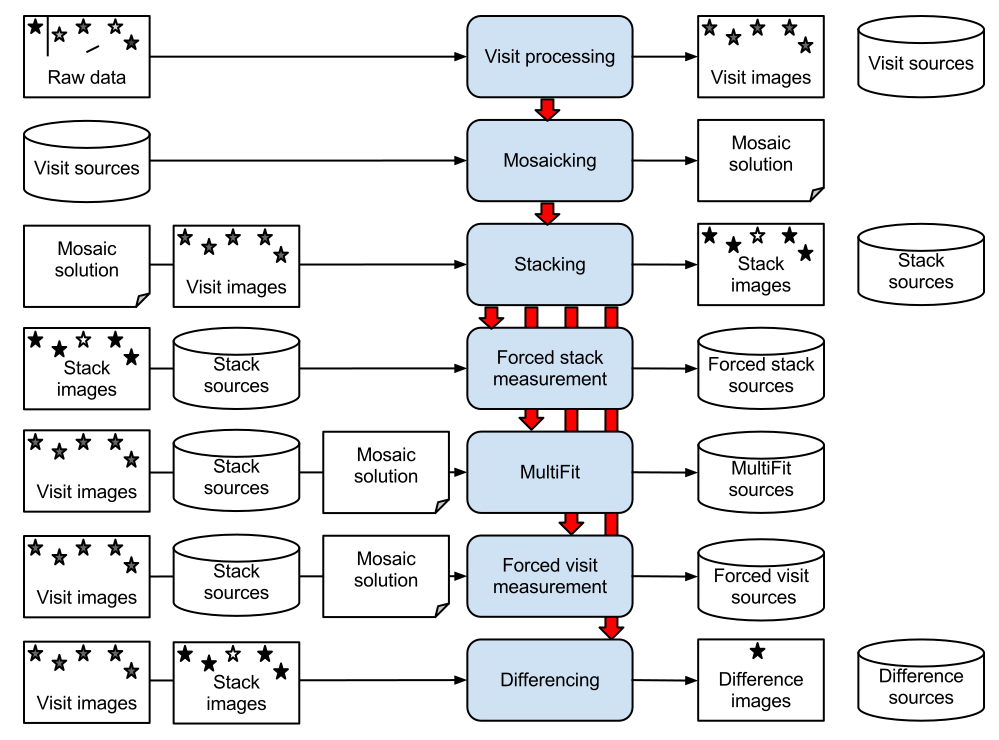
\includegraphics[scale=0.5]{figures/HSCpipelinesketch}
    \caption{HSC Pipeline data flow\label{fig:flow}}
\end{figure}

Figure~\ref{fig:flow} shows a schematic representation of the HSC pipeline.  Input data on the left is fed
into the pipeline stages (light blue, center) to produce the outputs on the right.  The first three stages
(visit processing, mosaic solution, stacking) are executed (red arrows) in sequence,
after which all the remaining stages
can be run in parallel.  The stages are explained in more detail below.

\subsubsection{Visit processing}

Visit processing removes the instrumental signature (overscan, bias, dark, flat, fringe (\S\ref{alg:fringe}),
bad pixels, amplifier
crosstalk) from each CCD and flags suspected cosmic-rays (\S\ref{alg:cosmicray}).  The result is a clean
image for which the intensity
is a linear function of astrophysical flux\footnote{Excepting flat-field inaccuracies, and intrinsic pixel
  shape non-linearities.}.  The background is estimated (\S\ref{alg:background}) and removed, then bright
sources on the image are used
to measure the PSF (\S\ref{alg:psf}), the astrometric solution and photometric zero-point, before a final
detection and
measurement pass covering all sources.  From the individual CCD measurements, we determine and apply an
exposure-wide astrometric
solution and photometric zero-point.

\subsubsection{Mosaic solution}

Once several exposures overlapping the same part of sky are available, we can determine a mosaic solution.
This involves solving for consistent astrometric solutions and photometric zero-points for the set of
exposures, using sources in common to multiple exposures, in the same manner as \citet{2008ApJ...674.1217P}.
This allows increased accuracy and precision relative to the visit processing, by allowing use of the many stars
fainter than in our original reference catalog (e.g., SDSS), and incorporating spatial information unavailable
from single exposures.  For further details on the algorithm and functional form, see \S\ref{alg:mosaic}.


\subsubsection{Stacking}
\label{flow:stack}

Stacking involves the coaddition of multiple images to produce a single, deeper image.  We apply the results
of the mosaic solution to the input images, warp (\S\ref{alg:warp}) them to a common coordinate system
(``sky map'';
\S\ref{alg:skymap}) and stack the pixels.  Then we detect and measure sources on the stack.  Our code
includes a couple of recent innovations to increase the quality of the stacks: background maching and
CoaddPsf.

Stacks are normally produced by first subtracting the background, but determining the background from
individual visits separately is problematic (because different choices can be made in each, especially at
the edge of a CCD; and because extended, faint astrophysical flux is misinterpreted as background), commonly
manifesting
as dark rings around bright stars and galaxies.  Instead, we perform ``background matching''
(\S\ref{alg:backgroundMatching}) to produce a stack with a high signal-to-noise realization of the background
in a single reference exposure.  This background can then be measured over large scales and subtracted with a
high degree of accuracy.

It must always be remembered that a stack is a computational convenience, rather than a perfectly accurate
representation of the sky.  Indeed, if the seeing is not constant it becomes impossible to produce a
stack with a PSF varying in a continuous fashion over the field, unless we deliberately degrade the data by
convolving the inputs to a common PSF.  In order to attempt to deal with the discontinuous PSF, we use a
``CoaddPsf'' (\S\ref{alg:coaddPsf}), which is a sum of the PSFs of the input images at each point of interest.

Unfortunately, degrading the PSF is the only way of accurately measuring the colors of galaxies (e.g., for
photometric redshifts) from stacks in the presence of color gradients, seeing changes and imperfect galaxy
models.  For this reason, we
will produce ``PSF-matched stacks'' for the purpose of measuring galaxy colors.  But because these data have
been deliberately degraded, they are not the deepest available, so we will also produce ``deep stacks'' by
coadding without PSF matching.

Despite the intrinsic limitations of stacks, the measurements from this pipeline stage will be useful for
applications where extreme accuracy isn't required, e.g., searching for sources with extreme spectral features
such as high-$z$ quasars.  The deep stacks will also be used to identify discrete astrophysical objects for
the following stages that require known object positions and reference apertures.

\subsubsection{Forced Stack Measurement}

The deep stack catalog of a nominated band (e.g., $i$-band) will be used as a reference to measure sources in
PSF-matched stacks, with the same centroids and apertures.  This provides matched-aperture galaxy colors,
e.g., for photometric redshifts.  Because of the limitations of the stacks, these may not be the most accurate
measurements available, but they are more simple and will be available earlier than the full MultiFit
(\S\ref{flow:multifit}) measurements.

\subsubsection{Forced Visit Measurement}

The deep stack catalog of a nominated band (e.g., $i$-band) will be used as a reference to measure the sources in
every available visit.  This produces time-resolved positions (for proper motions and parallax) and fluxes
(for light curves).  These results may be preferred over photometry from the Differences stage for some
science goals, if the variable sources are not confused with other sources (e.g., variable stars and AGN;
not for SNe superposed on a host galaxy).

\subsubsection{MultiFit}
\label{flow:multifit}

%%%
%%% Contribution from Jim Bosch
%%%
For some measurements --- particularly shape measurement for weak
lensing --- measurement on a coadd image may not provide the necessary
precision and control of systematics.  To perform these measurements,
we will use what we call a ``MultiFit'' approach, in which a
parametrized model for each astronomical object is fit simultaneously
to all of the data in which that object appears.  Rather than
transform and combine the data, we instead transform the model to the
coordinate system of each exposure, convolve it by the appropriate
PSF, and compare it to the data from that exposure.  Measurements from
the coadd will be used as a starting point, so the multifit processing
will proceed by iterating over the catalog generated from the coadd,
loading postage stamps from the original images, and fitting to these
data.  Note that the output measurements will generally have the same
form as the coadd-based measurements - one set of measurements per
astronomical object; there is a single set of the
parameters that describe each object, not a different set of parameters
for each exposure in which it appears.

Because it does not involve transforming noisy data (which is usually
lossy in some sense), and instead transforms analytic models, a
multifit approach is theoretically optimal for measurements that can
be framed as the results of model-based fits to the data (note that
not all measurements can be framed in such a way, but those that
cannot usually do not properly account for the PSF).  While it may be
possible to construct an optimal coadd that would also be
theoretically optimal, we expect that the difficulty in creating such
a coadd (i.e. perfectly tracking the covariances between pixels
introduced by resampling to a common pixel grid) would be prohibitively
complex.  On the other hand, for many measurements a non-optimal coadd
(as described in \S\ref{flow:stack}) may be practically
sufficient, in the sense that the improvement produced by a
multifit-based measurement of the same would be negligible.  In these
cases, the coadd measurement is likely to be far more efficient
computationally.  Whenever possible, then, we will do as much work as
possible on the coadd first, and only use a multifit approach to ``tune up''
the final result.  And when this final tuning is determined to be
unnecessary, it can be skipped entirely.

The details of the algorithms we will use with the multifit approach
are still uncertain.  We will almost certainly include some sort
of Sersic-based galaxy modelling, likely with both bulge and disk
components, but we may hold some parameters or ratios of parameters
fixed.  This will provide one of our two main approaches to
computing galaxy colors (the other will be galaxy model fits to
PSF-matched coadds), and will constitute one of many appproaches to
shape measurement for weak lensing.  It is also unclear yet whether
these fits will be standard maximum-likelihood fits or a Bayesian
approach that involves sampling from the full likelihood surface
\citep{BA2013,Miller2013}.



\subsubsection{Differencing}

The deep stack images will be used as references to be subtracted from individual visits (or
nightly/monthly/yearly stacks of visits) in order to identify and measure transients.  We will use PSF matching
(\S\ref{alg:psfMatching}) to minimize false positives, but further work will be needed to produce a clean
candidate list.

At the present time, the differencing stage has been greatly neglected in the development of the pipeline, as
more fundamental operations have received priority.  We have prototype code for PSF matching that needs to be
cleaned up, made more robust, and thoroughly tested.  Nevertheless, we are committed to delivering the
differencing stage in advance of the second year of operations for the supernova/transient campaign.


\subsection{Releases}

Data releases are the culmination of the pipeline development and operations, whereby the results are delivered
to the collaboration for science use.

\tbd{The following suggested release types need discussion among the collaboration, and approval by the
  executive board.}

\subsubsection{Daily transients}

When particular observations have been declared by the transients working group as useful for the
identification of transients (SNe, GRBs), we will attempt to process those observations promptly through a
limited set of the pipeline stages --- visit processing, forced CCD measurements and differencing --- and
deliver the results to the transients working group by 4pm Hawaiian Standard Time the following day.  {\bf It
  should be understood that these releases will be preliminary, and made on a best-efforts basis.}  The
released data will be in the form of FITS images and FITS tables, using the pipeline's internal formats, and
will be placed in a suitable location for bulk download by the transients working group members.

\tbd{Need discussion with transients group on requirements
and manpower and processing power.}

\subsubsection{Dirty preview}

Aware of the great interest in the HSC survey observations by the collaboration members, and desiring to
encourage independent quality analyses, we will endeavor to produce a preview of the processed data (through
all the pipeline stages) to the collaboration as soon as possible after each observing run.  {\bf It should
be understood that these releases will be preliminary, and made on a best-efforts basis.}  The released data
will be in the form of FITS images for bulk download and a database accessed in the usual manner
(\S\ref{sec:database}).

Once the survey is sufficiently progressed that a single month's data is not as interesting, this type of
release may be suspended.

\tbd{This needs further thought and discussion as to its necessity and practicality.}

\subsubsection{Semi-annual}

The semi-annual releases are the main goal of the pipeline operations.  As part of each, it is our intention to
re-reduce all data from the survey with the best available code and calibrations, delivering all the data
products (\S\ref{sec:products}) to the survey collaboration.  Each semi-annual release will be formally
announced on the HSC mailing list\footnote{\email{hsc@astro.princeton.edu}}, and accompanied by a set of
release notes identifying features and known bugs\footnote{We guarantee that no release will be free of bugs.}
in the release.  The released data may be accessed through the methods described in \S\ref{sec:access}.


\subsubsection{World}

Pulbic world releases will consist of a previous semi-annual release to the collaboration, with password
restrictions lifted.

\section{Data Products}
\label{sec:products}

Here we describe the various data products produced by the pipeline.

\subsection{Images}

Images from the pipeline shall be multi-extension FITS (MEF) files, containing the image data, mask plane and
variance plane.  The World Coordinate System (WCS) in the headers shall use the \code{TAN-SIP} convention
\footnote{\url{http://fits.gsfc.nasa.gov/registry/sip.html}}, except for those corresponding to a tract/patch
(\S\ref{alg:skymap}) which shall use the standard \code{TAN} projection.  The FITS files may also contain
further extensions (e.g., for the PSF).  We encourage the use of our software in reading and manipulating the
files.

The mask planes are listed in the mask HDU header (with prefixes \code{MP_}).  The symbolic names correspond
to:
\begin{itemize}
\item \code{BAD}: the detector pixel is believed to be bad (e.g., non-functional, un-calibratable, or
  significantly vignetted).
\item \code{SAT}: the pixel was over the full well depth, and therefore likely leaked charge to its neighbors.
\item \code{INTRP}: the pixel value has been derived from interpolating from neighbors, and therefore does
  not properly represent the original value, e.g., if it was originally saturated or flagged as a cosmic ray.
\item \code{CR}: the pixel is believed to be contaminated by a cosmic ray hit.
\item \code{EDGE}: the pixel is close to the edge of the detector, and therefore the source detection threshold will be higher than usual; this has also been used to flag pixels in stacks that have no known value.
\item \code{DETECTED}: the pixel contains a source that has been detected.
\item \code{DETECTED_NEGATIVE}: the pixel contains a negative source that has been detected (usually in the
  difference stage).
\item \code{SUSPECT}: the pixel is non-linear.
\item \code{UNMASKEDNAN}: the pixel contained a \code{NaN} (not-a-number) value that has been suppressed.
\item \code{SYMM_1SIG}, \code{SYMM_3SIG} and \code{MONOTONIC_1SIG}: these are set in the deblender, as an aid
  in determining object shapes.
\end{itemize}

The images are provided principally for the sake of verifying candidates, quality analysis, and to enable
extensive analyses not supported by the pipeline.  If you desire the images in order to generate your own
catalogs (e.g, with SExtractor), please consider using the pipeline catalogs instead, as this will benefit
everybody (e.g., you will have regular updates with the latest code, and any problems you find can be used to
debug the pipeline).  If the particular measurement you desire to have is not available, please let us
know so that we can attempt to support it.

\subsubsection{Visits}

The visit images shall be a single MEF for each CCD, which is background-subtracted with the mosaic solution
(\S\ref{alg:mosaic}) applied.  The MEFs shall also include PSF models
for each.  The background model is saved separately, and available if desired.

\subsubsection{Stacks}

The stack images shall be a single MEF for each patch, with a pre-defined astrometric solution and photometric
zero point.  The MEFs shall also include a CoaddPsf (\S\ref{alg:coaddPsf}) for each.

\subsubsection{Differences}

The difference images shall be a single MEF for each patch, with a pre-defined astrometric solution for each,
and a photometric zero point calculated from the original visit.  The MEFs shall also include a suitable PSF
model for each.

\subsection{Catalogs}

The catalogs are the principal data product produced by the pipeline.  It is our goal that most of the science
projects of the survey collaboration can be performed almost entirely from the catalogs; this was the
experience for SDSS.  We encourage collaboration members to discuss with us the addition of particular
measurements or flags that are lacking in the catalogs, so that we can develop and include them.

Catalogs are stored internal to the pipeline as FITS tables.  In these tables, the flags are combined into
a single bit array (FITS format code \code{X}); your software may or may not recognize the flag names in the
header.  In general, it should not be necessary for those outside the pipeline team to read these FITS tables,
as the database (\S\ref{sec:database}) should contain all the same information.

The following measurements will be made for all processing stages:
\begin{itemize}
\item SDSS centroid (\code{centroid.sdss}; \S\ref{alg:centroid.sdss}), with error estimate
  (\code{centroid.sdss.err}).
\item Flux from PSF photometry (\code{flux.psf}; \S\ref{alg:flux.psf}), with error estimate
  (\code{flux.psf.err}).
\item Flux from sinc photometry (7 pixel radius; \code{flux.sinc}; \S\ref{alg:flux.sinc}), with error estimate
  (\code{flux.sinc.err}).
\item Flux from multiple \tbd{elliptical?} apertures (0.5, 0.75, 1.0, 1.5, 2, 3.0, 5.0 arcsec radii;
  \code{flux.aperture}), with error estimates (\code{flux.aperture.err}).
\item Kron flux (\code{flux.kron}; \S\ref{alg:flux.kron}), with error estimate (\code{flux.kron.err}).
\item Petrosian flux (\code{flux.petrosian}; \S\ref{alg:flux.petrosian}), with error estimate
  (\code{flux.petrosian.err}).
\item Gaussian model flux (\code{flux.gaussian}; \S\ref{alg:flux.gaussian}), with error estimate
  (\code{flux.gaussian.err}).
\item SDSS adaptive moments (\code{shape.sdss}; \S\ref{alg:shape.sdss}).
\item Star/galaxy indicator (\code{classification.extendedness}; \S\ref{alg:star-galaxy}).
\end{itemize}

\subsubsection{Visits}

No additions over the standard set.

\subsubsection{Stacks}

Because we use a CoaddPsf (\S\ref{alg:coaddPsf}), the flags regarding the PSF will not be populated.

In addition to the standard set, we will also measure:
\begin{itemize}
\item Shapes from the HSM regaussianization method (\code{shape.hsm.regauss.*}; \S\ref{alg:shape.hsm}).
\item Flux and shapes from the MultiShapelet algorithm (\code{multishapelet.*}; \S\ref{alg:multishapelet}).
\end{itemize}

\subsubsection{Forced Visit Measurements}

We will perform the standard set of measurements, except that the Kron, Petrosian and Gaussian fluxes will be
measured with apertures defined from the reference frame.

\subsubsection{Forced Stack Measurements}
\label{sec:forced-stack-measurements}

In addition to the standard set, we will also measure:
\begin{itemize}
\item Fluxes from MultiShapelet algorithm (\code{multishapelet.exp.flux}, {multishapelet.dev.flux},
  \code{multishapelet.combo.flux}; and associated errors).
\end{itemize}

The Kron, Petrosian, Gaussian and MultiShapelet fluxes will be measured with the aperture defined from the
reference frame.

\subsubsection{MultiFit}

In addition to the standard set, we will also apply:
\begin{itemize}
\item MultiShapelet algorithm \tbd{details TBD}.
\end{itemize}

%%%
%%% Contribution from Jim Bosch
%%%
As noted in \S\ref{flow:multifit}, the output catalogs
produced by multifit-based measurement algorithms will have the same
form as those produced by coadd-based measurement algorithms.  In
particular, there will not be any per-exposure information in the
multifit outputs, despite the fact that the measurements will fit the
model to the original exposure-level data.

However, it should be noted that the forced measurements discussed in
\S\ref{sec:forced-stack-measurements} could be performed either by
iterating over exposures and looking up the associated detections from
the coadd (as has been described above) or by iterating over all coadd
detections and fitting to the associated postage stamps from
individual exposures (as is done with multifit).  Which of these
approaches we actually take should be considered an implementation
detail, and will not change the outputs described in
\S\ref{sec:forced-stack-measurements}.

\subsubsection{Differences}

No additions over the standard set.

\subsection{Database}
\label{sec:database}

The database tables of HSC data are separated into two types: tables containing image metadata
for CCDs or coads; and tables containing objects detected and measured
on these images. After the production of the FITS files with the HSC pipeline, these will be
ingested into the database.  The database engine
for the HSC data is PostgreSQL (version 9.2 or later is recommended), which is one of the most
popular RDBMS\footnote{Relational DataBase Management System} in Japan.

Each of the tables in the database is listed below, with a brief description.  The full schema is
provided in \S\ref{sec:schema}.

\tbd{The database tables use a different vocabulary than in the rest of this document, e.g.:
``frame'' = processed CCD from visit processing stage, ``mosaic'' = coadd from stack processing stage.
One or the other needs to be updated.  Comments about which vocabulary is most helpful to science users
is welcome.}

\subsubsection{Tables for image metadata}

Meta data which will be injected into database tables are basically extracted from FITS header
in each image data and some additionals like celestial coordinates of 4-corners of image data
will be calculated based on these meta data.

\begin{itemize}
\item \code{Frame}:
metadata of reduced CCD images (visit processing stage), including filter names, time of exposure,
image quality information (e.g., seeing), astrometric and photometric information, etc.

\item \code{Frame_Mng}:
reduced CCD image data management, including location of the data, MD5, proposal ID,
and some other information required for data management.

\item \code{Frame_Hpx11}:
stores order 11 HEALPix indices which are used to cover the area occupied by the image. There are
multiple records for each CCD image.

\item \code{Exposure}:
metadata of each exposure, generally derived from statistics (e.g., average/rms of seeing,
photometric zero points, etc.) of reduced CCD image properties.

\item \code{Exposure_Mng}:
exposure metadata file management.

\item \code{Mosaic}:
metadata of coadd images (stack processing stage).

\item \code{Mosaic_Mng}:
coadd image data management, including the location of the data, MD5, proposal ID,
and some other information required for data management.

\item \code{Mosaic_Hpx11}:
stores order 11 HEALPix indices which are used to cover the area occupied by the coadd image.
There are multiple records for each coadd image.
\end{itemize}

\subsubsection{Tables for Object Catalog}
The tables for object catalog contain measured source positions, fluxes, shapes and flags.

\begin{itemize}
\item \code{Frame_Matchlist}:
contains matched objects in astrometric/photometric reference catalog (e.g., SDSS-DR8) on the reduced
CCD images.

\item \code{Frame_MatchCoordPhoto}:
contains the derived information like magnitudes and celestial coordinates of matchlist
objects, which are in \code{Frame_Matchlist} table.

\item \code{Frame_SourceList}:
contains objects which are detected/measured on the reduced CCD images (visit processing stage).

\item \code{Frame_SourceCoordPhoto}:
contains the derived information like magnitudes and celestial coordinates of sourcelist
objects, which are in \code{Frame_Sourcelist} table.

\item \code{Frame_Forcelist}:
contains measurements from forced CCD measurement.

\item \code{Frame_ForceCoordPhoto}:
contains the derived information like magnitudes and celestial coordinates of forcelist 
objects, which are in \code{Frame_Forcelist} table.

\item \code{Mosaic_Matchlist}:
contains the matched objects in astrometric/photometric
reference catalog (e.g., SDSS-DR8) on the coadd images.
It is currently not implemented.

\item \code{Mosaic_MatchCoordPhoto}:
contains the derived information like magnitudes and celestial coordinates of matchlist
objects, which are in \code{Mosaic_Matchlist} table. It is currently not implemented.

\item \code{Mosaic_SourceList}:
contains measurements from the coadd images (stack processing stage).

\item \code{Mosaic_SourceCoordPhoto}:
contains the derived information like magnitudes and celestial coordinates of sourcelist
objects, which are in \code{Mosaic_Sourcelist} table.

\item \code{Mosaic_Forcelist}:
contains measurements from forced stack measurement.

\item \code{Mosaic_ForceCoordPhoto}:
contains the derived information like magnitudes and celestial coordinates of forcelist
objects, which are in \code{Mosaic_Forcelist} table.

\item \code{Photoobj_Frame}:
summary table of objects which are in \code{Frame_Forcelist} table. One record is 
for one celestial object which have multiple entries of magnitudes/coordinated coming from all 
measurement regarding to the object. The unique ID which comes from the forced photometry reference 
will be used for gathering the all information on one celstial object mutiply measured in different 
exposures. 

\item \code{Photoobj_Mosaic}:
summary table of objects which are in \code{Mosaic_Forcelist} table. One record is 
for one celestial object which have magnitudes/coordinated coming from coadd images with different 
filters. The unique ID which comes from the forced photometry reference will be used for gathering 
the all information on one celstial object mutiply measured in different coadd images. 

\end{itemize}

\section{Algorithms}
\label{sec:algorithms}

Here we describe the various algorithms used within the pipeline.  Of particular interest are the flags
(\S\ref{alg:flags}) and measurements (\S\ref{alg:measurements}) that will comprise the source catalogs
produced in each pipeline stage, and be ingested into the database.  Then follows various general algorithms
used in the pipeline.

\subsection{Flags}
\label{alg:flags}

Flags are binary decisions for each object, indicating how measurements of that
object should be interpreted, and if they are trustworthy.

\subsubsection{Pixel flags}

Pixel flags are flags set on the basis of pixel characteristics.  They comprise:
\begin{itemize}
\item \code{flags.pixel.edge} is set if the source is near the edge of the frame (where the signal-to-noise
  requirement for detection is higher due to the convolution involved; and where measurements may be prone to
  failure).
\item \code{flags.pixel.bad} is set if any pixels in the source footprint have been masked as \code{BAD}
  (typically non-functioning detectors, or severely vignetted areas).
\end{itemize}

The following flags indicate whether the source has been affected by a variety of conditions.  There are two
modes for each: \code{<flag>.any} is set if any pixels in the source footprint have been affected (and
therefore measurements may be impacted only subtly if at all), while \code{<flag>.center} is set if
any pixels in the
$3\times 3$ region about the peak have been affected (and therefore measurements are likely drastically wrong).

\begin{itemize}
\item \code{flags.pixel.interpolated}: pixels masked as \code{INTRP}, i.e., have been interpolated over, and
  are therefore not the original pixels; this is done for saturated pixels and cosmic rays.
\item \code{flags.pixel.saturated}: pixels masked as \code{SAT}, i.e., are saturated (over full well depth).
\item \code{flags.pixel.suspect}: pixels masked as \code{SUSPECT}, i.e., are non-linear.
\item \code{flags.pixel.cr}: pixels masked as \code{CR}, i.e., suspected cosmic-ray.
\end{itemize}

The following set of flags is recommended to catch most problems a source will have:
\code{flags.pixel.interpolated.center|flags.pixel.saturated.center|
  flags.pixel.suspect.center|flags.pixel.cr.center}.  Of course, you should also check
the flag for the particular measurement algorithm of interest.

\subsubsection{Algorithm flags}

Each measurement algorithm (\S\ref{alg:measurements}) has a corresponding algorithm flag that, if set,
indicates the measurement failed; typically this means an exceptional conditional was encountered, such as the
source being too close to the edge.  These algorithm flags are named after the measurement with \code{.flags}
appended, e.g., \code{flux.gaussian.flags}.

\subsubsection{Calibration flags}

The following flags are set in the visit processing stage as part of calibrating the image:
\begin{itemize}
\item \code{calib.detected} is set if the source was detected in calibration (as a bright source).
\item \code{calib.psf.candidate} is set if the source was selected as a candidate PSF star.
\item \code{calib.psf.used} is set if the source was actually used in determining the PSF.
\end{itemize}

\subsubsection{Deblending flags}

The deblender records some details of the deblending through various flags and values in the catalog; see
\S\ref{alg:deblender}.  These allow blended sources to be identified and the family (parents, children,
siblings) to be identified.

\subsubsection{Stack flags}

Some additional flags are present for the stack processing stage, intended to help disambiguate overlaps
(see \S\ref{alg:skymap}):
\begin{itemize}
\item \code{detect.is-patch-inner} is set if the source is in the inner region of a patch (not in the
  intra-tract inter-patch overlap area).
\item \code{detect.is-tract-inner} is set if the source is in the inner region of a tract (not in the
  inter-tract overlap area).
\item \code{detect.is-primary} is set if the source has no children and \code{detect.is-patch-inner} and \code{detect.is-tract-inner} (i.e., should be considered as the primary stack detection of this source).
\end{itemize}

\subsubsection{Other}

\begin{itemize}
\item \code{flags.negative} is set if the source was detected as negative (principally used in the
  difference stage).
\item \code{flags.badcentroid} is set if the principal centroid algorithm (used to feed all other algorithms)
  failed.
\end{itemize}

\subsection{Measurements}
\label{alg:measurements}

The measurement framework we have developed is extensible, so that additional measurement algorithms can
easily be introduced (with only minor additions to the configuration files).  The current measurement
algorithms we use are described below.  The names used refer to the colum names in the catalogs produced by the
pipeline; \tbd{the mapping of these names to the database is not yet known}.

\subsubsection{Centroids}

Each centroiding algorithm provides the centroid (in a column named directly after the algorithm) and a packed
covariance matrix (\code{<algorithm>.err}); note that the covariance term ($\sigma_{xy}$) is often
\tbd{always?} unset.

\paragraph{centroid.sdss}
\label{alg:centroid.sdss}
The same centroiding algorithm as employed in SDSS \citep{SdssPhoto}, wherein the image is smoothed by the
PSF, and a Gaussian Quartic Interpolation is applied to the pixels surrounding the peak which, in particular,
works for critically-sampled images (whereas a simple parabolic fit does not).  The peak determination is
repeated with the smoothed image binned down, so that a reliable center is produced for extended sources.
David Monet (USNO) reports that this algorithm performs as well as {\sc SExtractor}, and it is our principal
centroider.

\paragraph{centroid.gaussian}
A Gaussian is fit to the source.  Despite originally being developed by David Monet (USNO) for astrometric
use, Monet reports this algorithm is inferior to the SDSS centroid algorithm.

\paragraph{centroid.naive}
A simple, unweighted first moment of the $3\times 3$ pixels around the peak.  This is not a very good centroider (it doesn't use the entire PSF), but is cheap.

\subsubsection{Shapes}

Shape algorithms should provide a shape (typically the 3 second moments; in a column named directly after the
algorithm) and a packed covariance matrix (\code{<algorithm>.err}).  However, because there are different
ways of measuring shapes, there is a diversity of measurements; when a measurement algorithm breaks from the
standard pattern, we detail the outputs.

\paragraph{shape.sdss}
\label{alg:shape.sdss}
The SDSS adaptive moments, whereby the second moments are measured iteratively, with a Gaussian weight with
size set from the previous iteration.

\paragraph{shape.hsm}
\label{alg:shape.hsm}
Various shape measurements intended for weak lensing, originally developed by \citet{2003MNRAS.343..459H} and
tested on SDSS by \citet{2005MNRAS.361.1287M}.  The PSF correction methods are:
\begin{itemize}
  \item \code{shape.hsm.ksb}: The KSB \citep{1995ApJ...449..460K} method.
  \item \code{shape.hsm.bj}: The BJ method from \citet{2002AJ....123..583B} Appendix~C.
  \item \code{shape.hsm.linear}: The ``linear'' method, a variation of method (b) described in Appendix B of \citet{2003MNRAS.343..459H}.
  \item \code{shape.hsm.regauss}: The ``re-Gaussianization'' method from Section~2.4 of \citet{2003MNRAS.343..459H} that has been extensively tested \citep{2005MNRAS.361.1287M, 2007MNRAS.376...13M}.
  \item \code{shape.hsm.shapelet}: A ``shapelet'' method, implementing \citet{2003MNRAS.338...35R}.
\end{itemize}
Each of these algorithms provide:
\begin{itemize}
\item \code{<algorithm>.centroid}: The centroid.
\item \code{<algorithm>.moments}: The uncorrected moments.
\item \code{<algorithm>.psf}: Moments of the PSF at the source position.
\item \code{<algorithm>.e1} and \code{<algorithm>.e2}: The ellipticity (\citealt{2002AJ....123..583B};
  \code{bj}, \code{linear}, \code{regauss}) or estimated shear (\code{ksb}, \code{shapelet}).
\item \code{<algorithm>.resolution}: Resolution factor (0 means unresolved, 1 means resolved).
\item \code{<algorithm>.sigma}: Width.
\end{itemize}

\paragraph{shape.miyatake}
A shapelet-based method described in \citet{2012arXiv1209.4643M}, which originates from
\cite{2002AJ....123..583B} and \cite{Nakajima:2006}.  This measurement provides:
\begin{itemize}
\item \code{shape.miyatake.centroid}: The centroid.
\item \code{shape.miyatake.psf}: Moments of the PSF at the source position.
\item \code{shape.miyatake.e1} and \code{shape.miyatake.e2}: Ellipticity.
\item \code{shape.miyatake.e1var}, \code{shape.miyatake.e2var} and \code{shape.miyatake.e1e2cov}: covariance matrix.
\item \code{shape.miyatake.sigmagal} and \code{shape.miyatake.ordergal}: Sigma and order for galaxy GL. \tbd{What is GL?}
\item \code{shape.miyatake.sn}: Signal-to-noise ratio.
\item \code{shape.miyatake.status}: Status code.
\end{itemize}

\subsubsection{Fluxes}
\label{alg:measurements-flux}

Each flux measurement algorithm provides a flux (\code{<algorithm>}) and corresponding error
(\code{<algorithm>.err}).

The zero-point of all fluxes is that of the sinc aperture flux, so that fluxes of point sources by each
algorithm should be equal.  This is done by fitting an aperture correction over the image for each flux
measurement, referenced to the sinc aperture flux.

\paragraph{flux.psf}
\label{alg:flux.psf}
A PSF flux: the total flux of the source, weighted by the PSF.

\paragraph{flux.sinc}
\label{alg:flux.sinc}
The total flux of the source within a specified aperture.  This is calculated using sinc interpolation so the
value is the exact amount within the aperture, rather than being scaled to a non-integral number of pixels
after summing only pixels lying entirely within the aperture \citep{2013MNRAS.431.1275B}.

\paragraph{flux.gaussian}
\label{alg:flux.gaussian}
The flux from fitting a Gaussian model, with shape defined by the adaptive moments (\code{shape.sdss}).

\paragraph{flux.kron}
\label{alg:flux.kron}
Flux using an elliptical aperture defined by \citet{1980ApJS...43..305K}: the Kron radius is measured as the
moment within an (elliptical) aperture of six times the (adaptive) moment, and the Kron flux is measured
within an (elliptical) aperture of 2.5 times the Kron radius.  The sinc algorithm is used on smaller sized
apertures (less than 10 pixels radius) to measure the exact
flux within this aperture.  The shape of the elliptical aperture is defined by the adaptive moments
(\code{shape.sdss}).  The Kron `radius' is the ``determinant radius'' ($\sqrt{ab}$, where $a$ and $b$ are the
semi-major and semi-minor axes).

\paragraph{flux.petrosian}
\label{alg:flux.petrosian}
Flux using an (elliptical) aperture defined by \citet{1976ApJ...209L...1P} and, implemented in the same manner
as described in Section~A3 of \citet{2002AJ....124.1810S}: the Petrosian radius is the radius, $r$, for which
the surface brightness within an (elliptical) annulus from $0.8r$ to $1.25r$ is 0.2 times the mean surface
brightness within $r$, and the Petrosian flux is measured within an (elliptical) aperture of twice the
Petrosian radius.  The shape of the elliptical aperture is defined by the adaptive moments
(\code{shape.sdss}).  \tbd{This measurement is not yet implemented in the pipeline, though prototype code
  exists somewhere.}

\subsubsection{MultiShapelet}
\label{alg:multishapelet}

%Model fluxes are determined from fitting PSF-convolved elliptical models to the source.  We fit separately a
%pure exponential model, a pure de\ Vaucouleur model, and a linear combination of these two models (neither
%component is allowed to be negative, and the ellipses are fixed, so this is not quite a true bulge-disk
%decomposition).  This is similar to the SDSS ``cmodel'' fluxes \citep{SdssPhoto}, except that the profiles are
%constructed approximately from sums of Gaussians (8 for each profile; \citealt{HoggLangMoG}), and are
%convolved with a shapelet approximation of the PSF.

PSF-convolved galaxy models are a major
component of both galaxy flux measurements and shape
measurement for weak lensing.  Convolving and evaluating these models
on a pixel grid is both computationally expensive and difficult from
an accuracy perspective, so as a baseline approach we have adopted the
methods of \cite{HL2013} and \cite{Bosch2010}, in which a fixed-slope
Sersic profile is approximated by a sum of Gaussians,
and convolved analytically with a PSF model approximated as a sum of
multi-scale shapelet functions.  Aside from speed, a major advantage
of this approach is its transparency: while we must approximate both
the galaxy profile and the PSF model, these approximations are
explicit, and we can increase the fidelity of both in a
straightforward way.  Alternative methods that involve convolutions in
real-space or Fourier-space involve difficult decisions with much less
clear impacts on the fidelity of the models, involving how to
handle the wide range spatial frequencies caused by the cuspy cores
and broad wings of realistic galaxy profiles.

One distinct disadvantage of this ``multishapelet'' approach to galaxy
modeling construction is that it cannot easily handle Sersic models in
which the Sersic index is a free parameter; the sum of Gausssians that
approximates a Sersic profile with a certain Sersic index must be
precomputed.  We can fit linear combinations of fixed-index Sersic
profiles, however, and these fits are signficantly more
numerically stable.  The linear combination amplitudes also show a tight
correlation with free-index Sersic \tbd{RHL: reference from SDSS?},
which may mean that true free-index Sersic fits may be unnecessary.

Exactly which models will be fit and which parameters will be allowed
to vary is a current research topic, but as a baseline we have
implemented the same approach used in the SDSS \code{cmodel} magnitudes
\citep{SdssPhoto},
in which a pure exponential and pure de Vaucouleur are each fit
separately, and then their linear combination is fit while the ellipse
parameters are held fixed.  We will also explore the two component
partial bulge+disk fit used in \cite{Miller2013}, in which the bulge
radius is a fixed fraction of the disk radius and the ellipticity of
both components are the same, as well as true bulge+disk fits with
more free parameters.  We may try models with more than two components
as well, in the hopes of providing an even better analogue to
free-index single-Sersic fits.

The output parameters for each of the \code{multishapelet} components
are shown below:

\paragraph{multishapelet.psf}

\begin{itemize}
\item \code{<algorithm>.inner}: Gauss-Hermite coefficients of the inner expansion of the PSF.
\item \code{<algorithm>.outer}: Gauss-Hermite coefficients of the outer expansion of the PSF.
\item \code{<algorithm>.ellipse}: Ellipse corresponding to the inner expansion of the PSF.
\item \code{<algorithm>.chisq}: Reduced $\chi^2$ of the final shapelet fit to the PSF.
\item \code{<algorithm>.integral}: Integral of the shapelet PSF model to infinite radius.
\end{itemize}

\begin{itemize}
\item \code{<algorithm>.flags}: general algorithm failure.
\item \code{<algorithm>.flags.maxiter}: the optimizer ran into the maximum number of iterations limit.
\item \code{<algorithm>.flags.tinystep}: the optimizer step or trust region got so small no progress could be
  made.
\item \code{<algorithm>.flags.constraint.r}: the best-fit radius was the minimum allowed by the constraint.
\item \code{<algorithm>.flags.constraint.q}: the best-fit axis ratio (b/a) was the minimum allowed by the
  constraint.
\end{itemize}

\paragraph{multishapelet.exp and multishapelet.dev}

\begin{itemize}
\item \code{<algorithm>.flux}: flux of multi-Gaussian approximation to the profile, integrated to infinite
  radius; and error.
\item \code{<algorithm>.ellipse}: half-light radius ellipse.
\item \code{<algorithm>.chisq}: reduced $\chi^2$.
\end{itemize}

\begin{itemize}
\item \code{<algorithm>.flags}: general failure.
\item \code{<algorithm>.flags.maxiter}: the optimizer ran into the maximum number of iterations limit.
\item \code{<algorithm>.flags.tinystep}: the optimizer step or trust region got so small no progress could be
  made.
\item \code{<algorithm>.flags.largearea}: the best-fit half-light ellipse area is larger than the number of
  pixels used.
\end{itemize}

\paragraph{multishapelet.combo}

\begin{itemize}
\item \code{<algorithm>.flux}: combined flux of the linear combination of fixed-profile models; and error.
\item \code{<algorithm>.devfrac}: fraction of total flux in the de Vaucouleur component.
\end{itemize}

\subsection{Source identifiers}

Source identifiers are integers (typically 64-bit) that identify a particular source.  For uniqueness, they
encode information about the image on which they were measured.

\subsubsection{Visit}

The leftmost 32 bits encodes the visit and ccd:

\code{idBase = visit*200 + ccd}

\code{visit = int((id>>32)/200)}

\code{ccd = (id>>32)%200}

\subsubsection{Stack}

The leftmost 37 bits encode the tract (specified by an integer), patch (specified by x and y integers) and
filter (indentified by a unique integer):

\code{idBase = (tract*2^13 + xPatch)*2^13 + yPatch)*8 + filterNum}

\tbd{This will need to be updated when we produce stacks at multiple epochs: include average MJD and
  time range in days (as a proxy for starting and ending dates).}

\subsection{Background Matching}
\label{alg:backgroundMatching}

This technique will be important for reaching the maximum depth in the Deep and Ultradeep fields.  We use the
algorithm of \citealt{2011arXiv1111.6958H}, extended to two-dimensional data.

The problem is that the common practise of subtracting the background from each input individually removes
features on moderate scales (such as the outer haloes of galaxies, and Galactic cirrus) and can be unstable
(especially when the features appear at the edge of a frame) causing increased noise.  Instead, we choose a
reference exposure, and match the backgrounds of each of the other exposures to the reference.  This is done
by subtracting the reference from each of the other exposures (which mostly removes astrophysical sources,
especially the extended sources which normally contaminate background measurement) and fitting a background
model to the difference between the backgrounds.  These models are then subtracted from the other inputs, so
that all exposures have the same large-scale background as the reference exposure.  After coaddition, the
stack will contain the extended astrophysical features we desire at high signal-to-noise, and the background
can be carefully removed over multiple patches at once.

The subtracted image also provides an opportunity to identify sharp features such as optical ghosts, glints
and other contaminants that can be masked.

\subsection{PSF}
\label{alg:psf}

We run separate algorithms to select candidate stars and determine the point-spread function (PSF, the light
distribution for a point source, a critical ingredient to understanding the data and measuring accurate
shapes).  Both the star selector and PSF determiner algorithms are pluggable, so that different algorithms can
be run as desired for different analysis needs.

The ``second-moment'' star selector, for example, builds a histogram of the X and Y second moments of flux,
searches for a peak, and selects sources in the peak as point source candidates.  The ``catalog'' star
selector, in contrast, uses an external catalog of point sources and uses astrometric matching to select point
source candidates.  The ``objectSize'' star selector (our current favourite, as of 2013 August) identifies
point source candidates from the cluster of sources with similar sizes regardless of magnitude.  When
selecting point source candidates by size (i.e., for the ``second-moment'' and ``objectSize'' algorithms), the
sizes are first corrected by the known optical distortion of the camera.

The ``principle-components'' PSF (pcaPsf) determiner, performs a singular value decomposition (also known as a
principal components analysis, or PCA) on the point-source candidates in pixel space to produce a set of
eigen-images.  From a subset of the dominant eigen-images, we construct polynomial interpolants for their
relative weights.  This produces a spatially-varying PSF model that captures the most important changes in the
PSF over the CCD.

We are currently (August 2013) investigating the use of other PSF models, including PSFEx
\citep{2011ASPC..442..435B}.


\subsection{CoaddPsf}
\label{alg:coaddPsf}

%Measurements on the stacks will use a PSF constructed from those of the input images (known as ``StackFit'',
%pioneered by \citealt{2012arXiv1210.2732J} on the Deep Lens Survey).  In this way, we can accurately follow
%the complicated (and discontinuously variable) PSF over the stacked image.  We expect these measurements will
%be scientifically useful in their own right, and they will be available relatively quickly, but will not be
%the most accurate possible because the stacking process necessarily discards data.

%%%
%%% Contribution from Jim Bosch
%%%
One of the main challenges in producing quality measurements from
non-PSF-matched coadds is the complexity of the effective point-spread
function on the coadd.  Because the PSF has discontinuities at the
location of chip boundaries, modeling approaches based on
interpolating with smooth functions cannot be used.  Instead, when
creating a coadd image, we also combine the PSF models of all the
input exposures, using an approach similar to that devised by
\cite{JT2011}.  This combination is lazy, in that we simply store the
PSF models, their bounding boxes, and the coordinate transforms that
relate them to the coadd pixel grid.  Then, when measuring an object
on the coadd, we obtain the coadd PSF model at that location by coadding the
PSF models of all exposures that contributed to the relevant part of
the coadd, after warping them by the appropriate coordinate
transform.  We approximate the PSF as spatially constant in the region
of an individual object.

This approach is not exact in the presence of missing data.  When a
particular exposure pixel does not contribute to the coadd, the
associated PSF should not contribute as well, but the cost of storing
a mask mapping these rejected pixels along with the PSF is currently
prohibitively expensive, so the PSF combination algorithm does not
consider rejected or masked pixels.  More importantly, when only
certain pixels that contribute to an object are rejected, the PSF
model on the coadd is not well-defined for that object; we cannot
represent the coadd as the convolution of an idealized astrophysical
object with any convolution kernel.  This is a particular problem for
stars that are near the saturation limit: if they are saturated in
some frames, but not others, accurate coadd measurements become
essentially impossible.  Cosmic rays will also contribute to this
effect for many more objects, but at a lower level, and objects whose
isophotes cross a chip boundary in one or more input exposures will
also be affected.  It is worth
noting that this requires coaddition to be based on a straightforward
mean with as little clipping as possible; both median
stacking and aggressive clipping will cause the PSF of the coadd to be
poorly-defined, and a poor match to the model produced by the CoaddPsf
approach.

\subsection{Skymap}
\label{alg:skymap}

The ``skymap'' is a tessellation of the sky, providing suitable pre-defined coordinate systems for operations
on the sky such as stacking.  The sky map divides the sky into ``tracts''.  For convenience and parallelism,
each tract is sub-divided into ``patches''.  Tracts and patches overlap, so that sources are not lost in the
gaps.  These overlaps can be both annoying (additional care is required to remove duplicate sources) and
useful (additional source of quality checking).

Our tracts tangent planes (\code{TAN} WCS) distributed in rings of Declination, which matches well with the
survey geometry.  This has more inefficiency (tract overlap) at the pole, but since our survey doesn't cover
that area, it's not a problem.  Individual tracts are roughly the same size as the field of view of HSC, and
have North and East vectors aligned with the columns and rows, respectively.

\begin{figure}[!htbp]
    \centering
    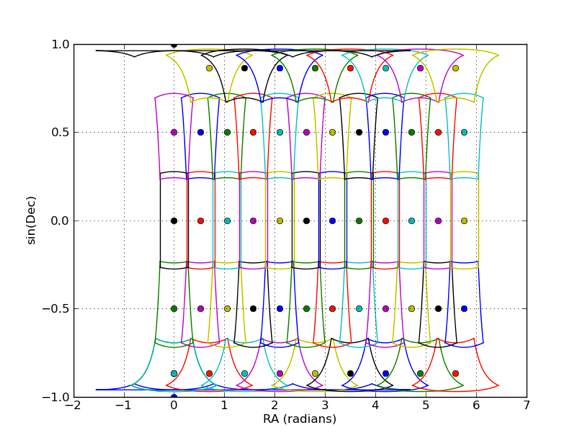
\includegraphics[scale=0.3]{figures/rings_equat.png}
    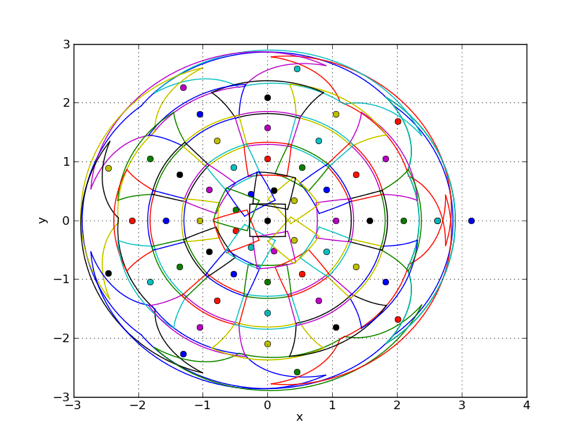
\includegraphics[scale=0.3]{figures/rings_pole.png}
    \caption{Demonstration of the skymap scheme we will use for the HSC pipeline.  Left: Equatorial
      projection.  Right: Polar projection.  Note that the tracts shown here are very much larger than we will
      use in practise; the large tracts allows the characteristics of the tessellation (e.g., the larger
      overlap at the poles) to be more clearly discerned.\label{fig:skymap}}
\end{figure}

\subsection{Mosaic}
\label{alg:mosaic}

For each exposure we can calibrate both astrometry and photometry using measurements of objects
matched with a reference catalog (e.g., SDSS), but this limits us to bright objects reference catalog and
we may be affected by some systematic effects. Simultaneously fitting multiple exposures enable a more
reliable and systematics free calibration. This is known as "uber-calibration" and
applied to SDSS \citep{2008ApJ...674.1217P} and Pan-STARRS1 \citep{2012ApJ...756..158S} photometry.
In the pipeline we apply the same kind of method
to each tract. "Uber-calibration" for entire survey region is a separate problem and not yet implemented.

We use both objects that have been matched with the reference catalog and non-matched objects.
Non-matched objects are matched between exposures based on astrometry determined
by chip based analysis. Requirements for non-matched objects having consistent positions/fluxes
contribute to better relative (internal) consistency and requirements for catalog matched objects
contribute to absolute (external) consistency.

In fitting the astrometry, the optical distortion of the system is modeled as polynomial functions of
focal plane coordinates.
We determine the coefficients of polynomials for each exposure. The locations of CCDs on the focal plane
(offsets and rotations) are also fitting parameters.
In fitting the photometry, a correction to the flat-field is modeled as polynomial functions of
focal plane coordinates.
We determine the coefficients of these polynomials in the same way as for the astrometry.  Relative flux
scales between exposures
are also determined.

The mathematical functional forms are as follows.
In the following, super(sub)scription $s$, $e$, and $c$ denotes stars, exposures and chips, respectively.
$(x,y)$ is a pixel coordinate within a chip, $(u,v)$ is a focal plane coordinate, $(\xi,\eta)$ is an projected
celestial coordinate of the sky at $(A,D)$.

For astrometry, we solve the equation for $\Delta a_k^e$, $\Delta b_k^e$, $\Delta X_c$, $\Delta Y_c$, and
$\Delta\theta_c$ until it converges. For non-matched sources, $\Delta\alpha^s$ and $\Delta\delta^s$ are also
solved.  For matched sources, the $(\alpha, \delta)$ are fixed to their catalog values.
The $\chi^2$ equation is linearized at eq (5). Initial values are estimated from the fit to matched sources for
individual exposures. Only multiply ($n\ge2$) observed non-matched sources are used in the fitting.

\footnotesize

\begin{equation}
\left(
\begin{array}{c}
u^{s,e} \\
v^{s,e} 
\end{array}
\right)
=
\left(
\begin{array}{cc}
\cos \theta_c & -\sin \theta_c \\
\sin \theta_c & \cos \theta_c
\end{array}
\right)
\left(
\begin{array}{c}
x^{s,e,c} \\
y^{s,e,c} 
\end{array}
\right)
+
\left(
\begin{array}{c}
X_c \\
Y_c
\end{array}
\right)
=
\left(
\begin{array}{c}
x^{s,e,c}\cos\theta_c-y^{s,e}\sin\theta_c+X_c \\
x^{s,e,c}\sin\theta_c+y^{s,e}\cos\theta_c+Y_c
\end{array}
\right)
\nonumber
\end{equation}

\begin{equation}
\left(
\begin{array}{c}
\xi^{s,e} \\
\eta^{s,e}
\end{array}
\right)
=
\left(
\begin{array}{c}
\xi(\alpha^{s}, \delta^{s}, A^{e}, D^{e}) \\
\eta(\alpha^{s}, \delta^{s}, A^{e}, D^{e})
\end{array}
\right)
\end{equation}

\begin{eqnarray}
\chi^2 & = & \sum_e \sum_s \left\{ \xi^{s,e}-\sum_k a_k^e [u^{s,e}]^{i(k)} [v^{s,e}]^{j(k)} \right\}^2 + \sum \left\{ \eta^{s,e}-\sum_k b_k^e [u^{s,e}]^{i(k)} [v^{s,e}]^{j(k)} \right\}^2 \\
& = & \sum_e \sum_s \left\{ \xi^{s,e}-\sum_k a_k^e [x^{s,e}\cos\theta_c-y^{s,c}\sin\theta_c+X_c]^{i(k)} [x^{s,e}\sin\theta_c+y^{s,c}\cos\theta_c+Y_c]^{j(k)} \right\}^2 \nonumber \\
& + & \sum_e \sum_s \left\{ \eta^{s,e}-\sum_k b_k^e [x^{s,e}\cos\theta_c-y^{s,c}\sin\theta_c+X_c]^{i(k)} [x^{s,e}\sin\theta_c+y^{s,c}\cos\theta_c+Y_c]^{j(k)} \right\}^2 \\
& = & \sum_e \sum_s \Biggl\{ \xi^{s,e} + \frac{\partial \xi^{s,e}}{\partial \alpha^{s}} \Delta\alpha^{s} + \frac{\partial \xi^{s,e}}{\partial \delta^{s}} \Delta\delta^{s}  \nonumber \\
&  & \hspace{0.7cm}- \left(\sum_k a_k^e [u^{s,e}]^{i(k)} [v^{s,e}]^{j(k)} \right. +\sum_k \Delta a_k^e [u^{s,e}]^{i(k)} [v^{s,e}]^{j(k)} \nonumber \\
&  & \hspace{1.0cm}+ \sum_k a_k^e \cdot i(k) \cdot [u^{s,e}]^{i(k)-1} [v^{s,e}]^{j(k)} \Delta X_c + \sum_k a_k^e \cdot j(k) \cdot [u^{s,e}]^{i(k)} [v^{s,e}]^{j(k)-1} \Delta Y_c \nonumber \\
&  & \hspace{1.0cm}+ \sum_k \Biggr[ a_k^e [u^{s,e}]^{i(k)-1} [v^{s,e}]^{j(k)-1}  \nonumber \\
& & \hspace{1.0cm} \{-i(k)[v^{s,e}](x^{s,e}\sin\theta_c+y^{s,e}\cos\theta_c)+j(k)[u^{s,e}](x^{s,e}\cos\theta_c-y^{s,e}\sin\theta_c) \} \Biggr] \Delta \theta_c \Biggr) \Biggr\}^2 \nonumber \\
& + & \sum_e \sum_s \Biggl\{ \eta^{s,e} + \frac{\partial \eta^{s,e}}{\partial \alpha^{s}} \Delta\alpha^{s} + \frac{\partial \eta^{s,e}}{\partial \delta^{s}} \Delta\delta^{s}  \nonumber \\
&  & \hspace{0.7cm}- \left(\sum_k b_k^e [u^{s,e}]^{i(k)} [v^{s,e}]^{j(k)} \right. +\sum_k \Delta b_k^e [u^{s,e}]^{i(k)} [v^{s,e}]^{j(k)} \nonumber \\
&  & \hspace{1.0cm}+ \sum_k b_k^e \cdot i(k) \cdot [u^{s,e}]^{i(k)-1} [v^{s,e}]^{j(k)} \Delta X_c + \sum_k b_k^e \cdot j(k) \cdot [u^{s,e}]^{i(k)} [v^{s,e}]^{j(k)-1} \Delta Y_c \nonumber \\
&  & \hspace{1.0cm}+ \sum_k \Biggr[ b_k^e [u^{s,e}]^{i(k)-1} [v^{s,e}]^{j(k)-1}  \nonumber \\
& & \hspace{1.0cm} \{-i(k)[v^{s,e}](x^{s,e}\sin\theta_c+y^{s,e}\cos\theta_c)+j(k)[u^{s,e}](x^{s,e}\cos\theta_c-y^{s,e}\sin\theta_c) \} \Biggl] \Delta \theta_c \Biggr) \Biggr\}^2 \\
& = & \sum_e \sum_s \left\{ A_x^{s,e} - \sum_k \Delta a_k^e [u^{s,e}]^{i(k)} [v^{s,e}]^{j(k)} - B_x^{s,e} \Delta X_c - C_x^{s,e} \Delta Y_c -D_x^{s,e} \Delta\theta_c + \frac{\partial \xi^{s,e}}{\partial \alpha^{s}} \Delta\alpha^{s} + \frac{\partial \xi^{s,e}}{\partial \delta^{s}} \Delta\delta^{s} \right\}^2 \nonumber \\
& + & \sum_e \sum_s \left\{ A_y^{s,e} - \sum_k \Delta b_k^e [u^{s,e}]^{i(k)} [v^{s,e}]^{j(k)} - B_y^{s,e} \Delta X_c - C_y^{s,e} \Delta Y_c -D_y^{s,e} \Delta\theta_c + \frac{\partial \eta^{s,e}}{\partial \alpha^{s}} \Delta\alpha^{s} + \frac{\partial \eta^{s,e}}{\partial \delta^{s}} \Delta\delta^{s} \right\}^2 \nonumber \\
\end{eqnarray}

\begin{equation}
A_x = \xi - \sum_k a_k [u]^{i(k)} [v]^{j(k)}
\end{equation}

\begin{equation}
A_y = \eta - \sum_k b_k [u]^{i(k)} [v]^{j(k)}
\end{equation}

\begin{equation}
B_x = \sum_k a_k \cdot i(k) \cdot [u]^{i(k)-1} [v]^{j(k)}
\end{equation}

\begin{equation}
B_y = \sum_k b_k \cdot i(k) \cdot [u]^{i(k)-1} [v]^{j(k)}
\end{equation}

\begin{equation}
C_x = \sum_k a_k \cdot j(k) \cdot [u]^{i(k)} [v]^{j(k)-1}
\end{equation}

\begin{equation}
C_y = \sum_k b_k \cdot j(k) \cdot [u]^{i(k)} [v]^{j(k)-1}
\end{equation}

\begin{equation}
D_x = \sum_k a_k [u]^{i(k)-1} [v]^{j(k)-1} \{-i(k)[v](x^s\sin\theta_c+y^s\cos\theta_c)+j(k)[u](x^s\cos\theta_c-y^s\sin\theta_c) \} 
\end{equation}

\begin{equation}
D_y = \sum_k b_k [u]^{i(k)-1} [v]^{j(k)-1} \{-i(k)[v](x^s\sin\theta_c+y^s\cos\theta_c)+j(k)[u](x^s\cos\theta_c-y^s\sin\theta_c) \} 
\end{equation}

For photometry, we solve for $f_{i,j}$, $dm^e$, and $m_0^s$. Here, $m_0^s$ is the true magnitudes of stars.
For catalog matched objects, $m_0^s$ is fixed to $m_{cat}^s$ to yield an absolute calibration.

\begin{equation}
\chi^2 =  \sum_e \sum_s \left\{ m_0^s - \Biggl( m^{s,e}+dm^e+\sum_{i+j\le n} f_{i,j} [u^{s,e}]^i [v^{s,e}]^j \Biggr) \right\}^2
\end{equation}

\normalsize

\begin{figure}[!htbp]
    \centering
    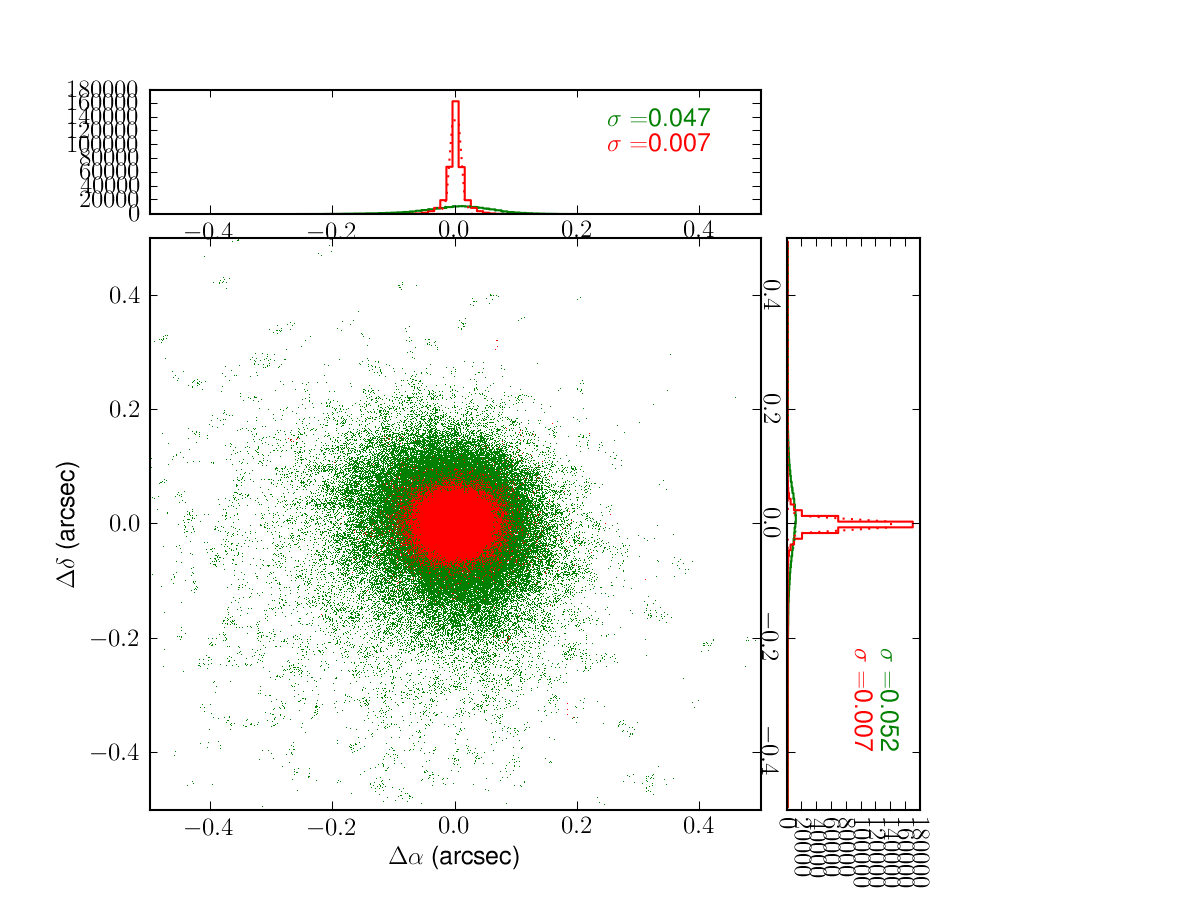
\includegraphics[scale=0.3]{figures/posScatter150.png}
    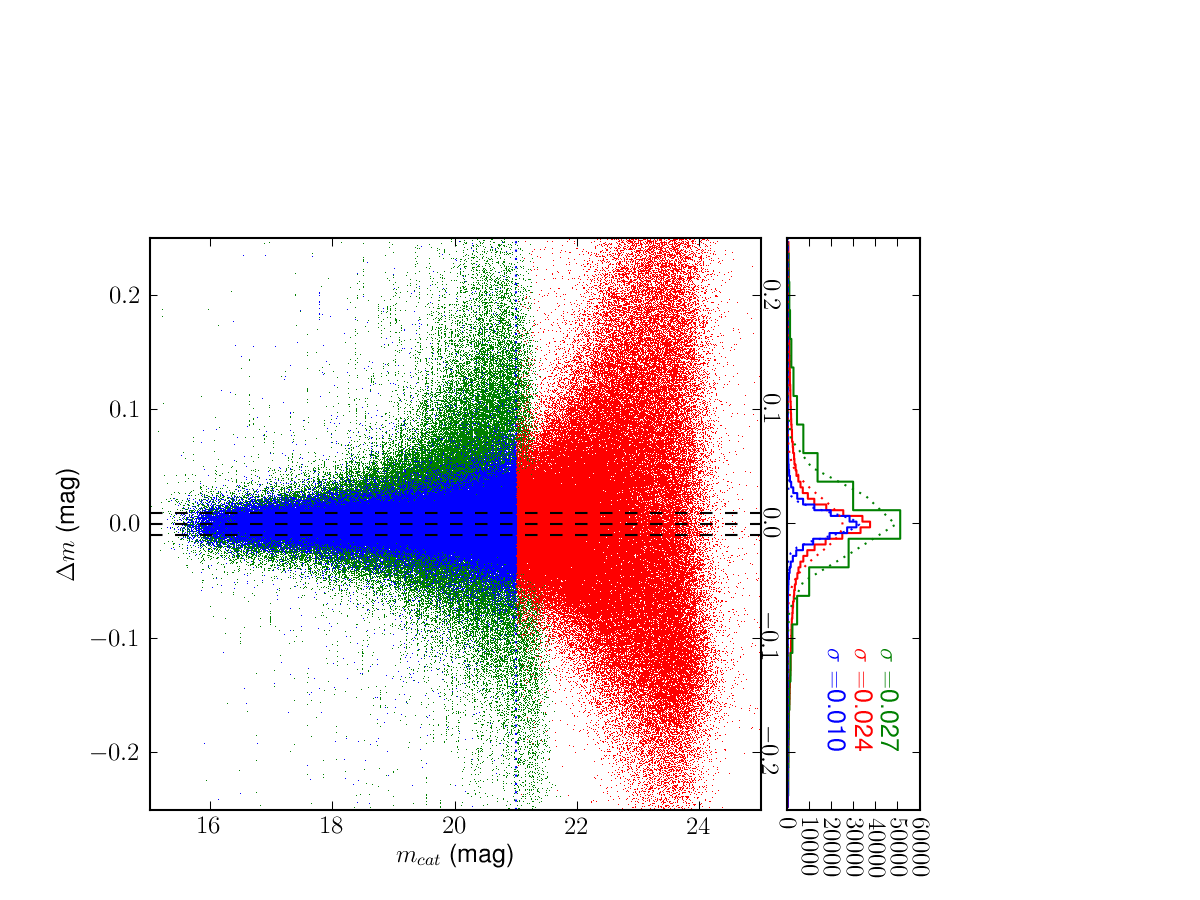
\includegraphics[scale=0.3]{figures/fluxScatter150.png}
    \caption{Results of mosaic solution for DITH-16H large dither
      dataset (4x4 visits).  In the astrometry plot (left), green points are external consistency
      (i.e., catalog matches; $\sim 50$~mas) and red points are internal consistency ($\sim 7$~mas).
      The same colors are used in the photometry plot (right; 27~mmag external, 24~mmag internal),
      and blue points are internal consistency only for bright objects (10~mmag).\label{fig:mosaic}}
\end{figure}



\subsection{PSF matching}
\label{alg:psfMatching}

PSF matching allows us to match the PSF of an input image to that of a target model or target image.  The
images with matched PSFs can be subtracted (to find transients) or coadded (to produce a stack with a PSF that
varies in a continuous manner over the image).  We use the algorithm of \citet{1998ApJ...503..325A} and
\citet{2000A&AS..144..363A}.  We have the option of using the traditional \citet{1998ApJ...503..325A}
Gaussian/polynomial basis functions, or regularised delta-function basis functions
\citep{2012MNRAS.425.1341B}.


\subsection{Deblending}
\label{alg:deblender}

At the depths probed by HSC images, many of the sources are superimposed on each other on the sky
(``blended''), which makes detecting and measuring such sources difficult.  Often this blending is not severe,
but the $5\sigma$ contours overlap (and therefore merge together) slightly.  In other cases, distinct objects
will be superimposed directly on more extended objects (e.g., a star on a resolved galaxy).  In order to
disentangle the multiple objects, we employ a ``deblender'' based on the experience of SDSS
\citep{2005ASPC..338..151L}.

The deblender assumes that discrete sources generally have twofold
rotational symmetry.  When one side of a source is blended, we can
recover its appearance by examining the symmetric side.  The deblender
begins by building these symmetric templates for each source.  Next,
the flux in each pixel is split among the blended source in proportion
to their templates.  The deblender produces ``postage stamps'' of each
source in a blended group, so that the measurement algorithms (fluxes,
galaxy shapes, etc) need not know that the source was blended.

This deblending algorithm works well in practise for moderately
crowded fields (as demonstrated by SDSS).

The deblender (\S\ref{alg:deblender}) sets the following flags based on its interpretation of the source:
\begin{itemize}
\item \code{deblend.deblended-as-psf} is set if the deblender considered the source as a PSF.
\item \code{deblend.too-many-peaks} is set if the deblender attempted to divide the source beyond a limit;
  only the brightest peaks were deblended.
\item \code{deblend.failed} is set if deblending failed on this source.
\end{itemize}

And the following values are set:
\begin{itemize}
\item \code{parent}: if non-zero, the \code{id} of the source from which this source was deblended.
\item \code{deblend.nchild}: the number of children this source was deblended into.
\item \code{deblend.psf-center}: the centroid of the PSF used, if \code{deblended-as-psf}.
\item \code{deblend.psf-flux}: the flux of the PSF used, if \code{deblended-as-psf}.
\end{itemize}

\subsection{Star/galaxy separation}
\label{alg:star-galaxy}

We perform star/galaxy separation based on the ratio of PSF and model fluxes:
\begin{itemize}
\item \code{classification.extendedness = (0.95*flux.gaussian < flux.psf) ? 0.0 : 1.0}
\end{itemize}


\subsection{Cosmic ray identification}
\label{alg:cosmicray}

We use the same algorithm as in SDSS to identify cosmic-rays by their morphology (see Section 4.3 of
\citealt{SdssPhoto}).  We have found this works well on the Hamamatsu thick CCDs in Suprime-Cam.

\subsection{Fringe subtraction}
\label{alg:fringe}

The Suprime-Cam data shows mild fringing in the $y$-band.  We construct fringes\footnote{This code fell out a
  little while ago, but it is easy to revive it.} by combining with rejection many night-time science
exposures.  To apply, the mean values are measured in a large number (e.g., 30,000) of randomly positioned
small regions (e.g., 10 pixels square), both on the fringe frame and the science frame, from which the relative
scaling of the fringe frame may be determined (with careful clipping to discard regions affected by
astrophysical sources).  The scaled fringe frame is then subtracted from the science frame.

\subsection{Background models}
\label{alg:background}

A smooth background is estimated and removed from the image.  We begin by measuring the background level in
cells (typically 256 or 512 pixels square) using (by default) a clipped mean, and ignoring pixels that are
part of detected sources.  We then construct an interpolating spline (Akima spline, by default) to estimate
the background level in each pixel.  Background models are saved, for later restoration (e.g., in background
matching, \S\ref{alg:backgroundMatching}).

\subsection{Warping}
\label{alg:warp}

In warping an image from the detector frame to the sky frame, we apply a resampling kernel.  The kernel is set
according to the sub-pixel position on the input image of the centre of the corresponding output pixel.  The
code supports using Lanczos (of configurable order), bilinear or nearest-neighbour kernels; we use a 3rd-order
Lanczos (with $10^6$ cache realisations), as a compromise between the infinite Sinc function and the need for
speed.

\subsection{Reference catalog}

The reference catalog used for forced measurement will be derived from detections and measurements on the
$i$-band coadd.

\tbd{We want to use $\chi^2$ coadds plus individual bands (e.g., to catch high-z quasars); do we need to worry
  about differences in deblending, etc.?}


\section{Data Access}
\label{sec:access}

Here we describe how the pipeline products can be retrieved by collaboration members, and ultimately the world.

\tbd{Note: We are currently prototyping a system, so this section is subject
  to change as the system design progresses.}

\subsection{Data Archive System (DAS)}
We provide a web-based user interface to retrieve the data products, including images and catalogs, detailed
in \S\ref{sec:products}.

\subsubsection{Servers in the system}
\begin{itemize}
\item {\bf Web Server} provides a graphical user interface to allow users 
(1) to search for necessary data products, and (2) submit a job to
post-process on products, and to download the products, and (3) monitor
status of the job execution. This server updates a job control table
for queueing jobs, and is also responsible for transferring files
to users' site.

\item {\bf Processing Server} executes jobs in the queue by
     referring to the job control table.

\item {\bf DB Server} holds the database, as described in \S\ref{sec:database}. Queries are processed on
  this server, based on the job table, too.

\item {\bf File Servers} are mounted over NFS from the DAS Web \&
     Processing Servers. All the data products are located on this
     server.
\end{itemize}

\subsubsection{Database}
The details of the database which stores meta information of data products
are described in \S\ref{sec:database}. We
employ a few tables (\code{*_Mng}), in a single database space, dedicated to tying file
paths in the system and identification numbers of products like (visit,
ccd, and processing rerun version).

Another database space for job control is created separately from the
products database. This database maintains user identification numbers
and status of job queueing with time stamps, and is used by the Job
Processing Server.

\subsubsection{Authentication}
We plan to apply LDAP authentication for user access control on a
user-by-user basis. By sharing the LDAP database with the Hilo base of
Subaru Telescope, the access right to the both DAS and CAS contents is
limited to only the registered collaboration members.

Each user is assigned their own temporary disk space (capacity
TBD; typically $<<$~1~TB). This space is a staging area which is used to store any files
output by queries and to be downloaded by a user, including 
symbolic links to the products, combined coadd images over a requested
sky patches on the fly, or catalog CSV files, etc.

\subsubsection{Job control and Backend Processes}
The maximum number of simultaneous processes are limited on each server,
for load balancing and stable operation of the system.

Web Server updates queued jobs in the job control table, and DB Server
processes the query jobs. Processing Server makes symbolic links to
images or combine the coadd images from multiple sky patches into a
single image per request.

\subsubsection{Graphical User Interface (GUI) and Available Data Search}
Currently, the DAS GUI provides users with the following functions of data retrieval:

\begin{enumerate}
\item Data search for Frame (CCD) and Mosaic (Coadd) products. These
     functions offer a simple data search in a typical basic condition
     for collaboration members.  The planned available options to query are filter
     name, observing date and time, and celestial coordinates (box
     search or radial cone search with respect to the given central (RA, Dec) coordinates).
\item Direct SQL search for Frame (CCD) and Mosaic (Coadd) products.
     In these windows, a user can feed their own SQL commands to the DB
     server.
     A quick syntax check is provided.
    Currently, the output is limited to 1000 rows and CPU time
     of only 3 sec, for demonstration purposes.
   We also plan to limit available SQL commands in order to prohibit unreasonable
    queries which consumes enormous CPU time of DB Server.
\item History of old queries. Any jobs submitted are recorded in users
     folder and are available in the later session as a template or
     for reprocessing a job.
\item Download of files. Once the files are stored in an individual
     staging area, a user can use \code{wget} to retrieve individual files or
     a set of queried products.
\item Monitor of queue status. Status of data requests can be monitored
     with the name of queue and processing status with relevant time stamps.
\end{enumerate}

\subsection{Catalog Archive System (CAS)}

The object catalogs will be served through a web-based user interface of the Catalog Archive
System (CAS).
We are currently designing and prototyping the minimal functions of CAS and
collecting collaboration members' requirements.
The detailed table relation and schema of the backend
catalog database is described in \S\ref{sec:database}.

\subsubsection{Graphical User Interface (GUI) and Available Data Search}

Currently, only a direct SQL search for catalog sources is
being tested, and several typical queries are available for the test.

We plan to provide the simple search mode for a typical
search condition which is similar to that in DAS.
Also, we plan to provide more thorough examples of SQL commands which will
be required for typical science cases.
Preparation of individual work spaces associated with a temporary
database (similar to SDSS' CASJobs), is under discussion.

In addition to the basic source search, the following functions are
available:
\begin{enumerate}
\item Quick Look Images of queried catalog sources. A user can toggle the
     viewing window of a quick look image (QLI) for searched sky area when
     available. This tool extracts the dumped JPEG image of
     coadded FITS data around the selected sources, and displays
     it onto the resultant window of the data search. When a certain
     source in the resultant list is clicked, a circle is plotted on
     the corresponding point on QLI.
\item Plotting tool. Any two parameters returned from the query can
     be plotted on a dedicated graph window; this is useful for quick
     verification of query results.
\item Downloading catalogs. Selected sources may be retrieved using the
     following file formats: CSV, SQLite database, and FITS BINTABLE.
\end{enumerate}


\section{Help and Support}
\label{sec:support}

The pipeline team is committed to supporting the collaboration in their understanding of the pipeline and the
use of its products.  To this end, there are two principal means of interacting with the pipeline team.  We
encourage collaboration members to use these means, rather than asking individual pipeline team members,
since they allow us to build up a body of support documentation that will be of use to the entire
collaboration.  In contrast, questions asked and answered privately do not benefit anyone else.

\subsection{Forum}

A web-based question-answer forum, similar to that of the popular coding forum \url{stackoverflow.com} has
been set up at \url{http://hsca.ipmu.jp:88/questions/}.  Collaboration members are encouraged to set up an
account and ask (and answer!) questions and vote on questions and answers.  Members of the pipeline team
receive e-mail notifications of postings, so that questions from collaboration members can be answered
promptly.  When you receive a suitable answer to your question, please ``accept'' it (by clicking on the check
mark to the left of the answer), so that everyone else can identify the correct solution.

\subsection{Mailing list}

The pipeline team (and interested bystanders) can be reached by e-mail to
\email{hsc_software@astro.princeton.edu}.  Collaboration members are welcome to sign up at
\url{http://jeeves.astro.princeton.edu/mailman/listinfo/hsc_software}.  The list archive is publicly
accessible, at \url{http://jeeves.astro.princeton.edu/pipermail/hsc_software/}


\clearpage

\bibliographystyle{SciBook}
\bibliography{description}

\appendix

\section{Database schema}
\label{sec:schema}

The current (as of August 2013) database schema is shown below, but is subject to change as the database is
developed.  For the most current version of the schema, please see the online schema browser:
\url{http://hsc-gw1.mtk.nao.ac.jp/schema_browser/hsc/hsc_online_schema_tableonly.html}

\tbd{Need to specify mapping between measurements (\S\ref{alg:flags}, \S\ref{alg:measurements}) and the
database columns.}

\tiny

\begin{deluxetable}{llllll}
  \tabletypesize{\tiny}
  \rotate
  \tablecolumns{6}
  \tablewidth{0pt}
  \tablecaption{Schema of {\tt Frame} table}
  \tablehead{
    \colhead{Column name} & \colhead{Data type} & \colhead{Description} & \colhead{Sample value} & \colhead{Unit} & \colhead{Comments}
  }
  \startdata
frame\_id & character varying(12) & Frame ID in FITS Header                             & HSC[A,B,C]????????         &             & FRAMEID  \\
frame\_num & integer & Number part of the Frame ID                         & \%9d                        &             &   \\
exp\_id & character varying(12) & Exposure ID in FITS Header                          & HSC[A,B,C]??????00         &             & EXP-ID  \\
exp\_num & integer & Number part of the Exposure ID                      & \%9d                        &             &   \\
ccd\_id & integer & CCD chip ID (DET-ID in FITS Header)                 & 0 - 103 ?                  &             & DET-ID  \\
rerun & text & RERUN ID                                            &                            &             &   \\
visit & integer & VISIT ID                                            &                            &             &   \\
ccd & integer & CCD chip ID extracted from FRAMEID                  & 0 - 103 ?                  &             &   \\
ccdname & character(3) & CCD chip ID in string                               & 1 ,  103 .....             &             &   \\
pointing & integer & Day number from a certain date                      &                            & Days        &   \\
ccdtemp & real & Temperature of CCD                                  &                            & Kelvin      & DET-TMP  \\
object & text & Object Name                                         &                            &             &   \\
naxis1 & integer & Length of Axis 1                                    &                            &             & NAXIS1  \\
naxis2 & integer & Length of Axis 2                                    &                            &             & NAXIS2  \\
bin\_fct1 & integer & Binning factor of axis 1                            &                            &             & BIN-FCT1  \\
bin\_fct2 & integer & Binning factor of axis 2                            &                            &             & BIN-FCT2  \\
ra & character varying(12) & Right Ascension (J2000.0) (Encoder Value)           & HH:MM:SS.SSS               &             & RA  \\
decl & character varying(12) & Declination (J2000.0) (Encoder Value)               & +/-DD:MM:SS.SS             &             & DEC  \\
equinox & real & Equinox                                             & 2000.0                     & Year        & EQUINOX  \\
ra2000 & double & Right Ascension of Frame Center                     &                            & Degree      &   \\
decl2000 & double & Declination of Frame Center                         &                            & Degree      &   \\
radecsys & text & System for RADEC description                        & FK5                        &             & RADECSYS  \\
ctype1 & text & Type of axis 1 WCS description                      & RA---TAN                   &             & CTYPE1  \\
ctype2 & text & Type of axis 2 WCS description                      & DEC--TAN                   &             & CTYPE2  \\
cunit1 & text & Unit of axis 1 WCS description                      & degree                     &             & CUNIT1  \\
cunit2 & text & Unit of axis 2 WCS description                      & degree                     &             & CUNIT2  \\
crpix1 & real & Reference pixel in axis 1                           &                            &             & CRPIX1  \\
crpix2 & real & Reference pixel in axis 2                           &                            &             & CRPIX2  \\
crval1 & double & Value of WCS in axis 1 at reference pixel           &                            & Degree      & CRVAL1  \\
crval2 & double & Value of WCS in axis 2 at reference pixel           &                            & Degree      & CRVAL2  \\
cd1\_1 & double & CD matrix                                           &                            &             & CD1\_1  \\
cd1\_2 & double & CD matrix                                           &                            &             & CD1\_2  \\
cd2\_1 & double & CD matrix                                           &                            &             & CD2\_1  \\
cd2\_2 & double & CD matrix                                           &                            &             & CD2\_2  \\
llcra & double & RA of lower left corner of ccd(frame)               &                            & Degree      &   \\
llcdecl & double & DEC of lower left corner of ccd(frame)              &                            & Degree      &   \\
ulcra & double & RA of upper left corner of ccd(frame)               &                            & Degree      &   \\
ulcdecl & double & DEC of upper left corner of ccd(frame)              &                            & Degree      &   \\
urcra & double & RA of upper right corner of ccd(frame)              &                            & Degree      &   \\
urcdecl & double & DEC of upper right corner of ccd(frame)             &                            & Degree      &   \\
lrcra & double & RA of lower right corner of ccd(frame)              &                            & Degree      &   \\
lrcdecl & double & DEC of lower right corner of ccd(frame)             &                            & Degree      &   \\
pa & real & Position Angle                                      &                            & Degree      &   \\
insrot & real & Angle of Instrument Rotator                         &                            & Degree      & INR-STR  \\
date\_obs & date & Observation Date (UT)                               & YYYY-MM-DD                 &             & DATE-OBS  \\
mjd & double & Modified Julian Date                                &                            & Day         & MJD  \\
taiobs & timestamp without time zone & Date-time of the observation                        & YYYY-MM-DD HH:MM:SS.SS     &             & DATE-OBS+UT  \\
ut & time without time zone & Universal Time                                      & HH:MM:SS.SS                &             & UT  \\
hst & time without time zone & Hawaii Standard Time                                & HH:MM:SS.SS                &             & HST  \\
lst & time without time zone & Local Siderial Time                                 & HH:MM:SS.SS                &             & LST  \\
azimuth & double & Azimuth angle                                       &                            & Degree      & AZIMUTH  \\
elevation & double & Elevation angle                                     &                            & Degree      & ALTITUDE  \\
airmass & double & Airmass                                             &                            &             & AIRMASS  \\
filter01 & text & Filter Name in FITS Header                          & W-S-R+  etc                &             & FILTER01  \\
filter & text & Filter Name used in Pipeline                        & r  etc                     &             & FILTER  \\
exptime & real & Exposure Time                                       &                            & Second      & EXPTIME  \\
data\_typ & text & Data Type (OBJECT, STANDARD\_STAR)                   & OBJECT                     &             & DATA-TYP  \\
gain1 & real & CCD Gain of section 1                               &                            &             & S\_GAIN1(SC)  \\
gain2 & real & CCD Gain of section 2                               &                            &             & S\_GAIN2(SC)  \\
gain3 & real & CCD Gain of section 3                               &                            &             & S\_GAIN3(SC)  \\
gain4 & real & CCD Gain of section 4                               &                            &             & S\_GAIN4(SC)  \\
da\_ver & text & Version of Data Analysis Software                   & HSCPIPE-1.12.0c\_hsc etc    &             &   \\
oslevel1 & real & Count Level of Over Scan 1(Median)                  &                            & ADU         &   \\
oslevel2 & real & Count Level of Over Scan 2(Median)                  &                            & ADU         &   \\
oslevel3 & real & Count Level of Over Scan 3(Median)                  &                            & ADU         &   \\
oslevel4 & real & Count Level of Over Scan 4(Median)                  &                            & ADU         &   \\
ossigma1 & real & RMS of Over Scan area 1                             &                            & ADU         &   \\
ossigma2 & real & RMS of Over Scan area 2                             &                            & ADU         &   \\
ossigma3 & real & RMS of Over Scan area 3                             &                            & ADU         &   \\
ossigma4 & real & RMS of Over Scan area 4                             &                            & ADU         &   \\
skylevel & real & Sky Count Level (Median)                            &                            & ADU         &   \\
sigma\_sky & real & RMS of Sky count                                    &                            & ADU         &   \\
flatness\_pp & real & Peak-to-Peak of median of segmented area            &                            & ADU         &   \\
flatness\_rms & real & RMS of median values of segmented area              &                            & ADU         &   \\
flatness\_ngrids & text & Number of grids used for flatness evaluation        &                            &             &   \\
flatness\_meshx & integer & Number of mesh in x-direction                       &                            &             &   \\
flatness\_meshy & integer & Number of mesh in y-direction                       &                            &             &   \\
seeing & real & Seeing size                                         &                            & pixel       &   \\
ellipt & real & Ellipticity of point source                         &                            &             &   \\
ell\_pa & real & Position angle of derived PSF                       &                            &             &   \\
wcs\_nobj & integer & Number of objects used for astrom calibration       &                            &             &   \\
wcs\_siporder & integer & Order of SIP polynomial                             &                            &             &   \\
wcs\_rms & real & RMS in astrometric fitting (ref. vs source)         &                            & arcsec      &   \\
zeropt & real & Zero point for the  frame (from FLUXMAG0)           &                            & mag         & 2.5*log10(FLUXMAG0)  \\
magzero & real & Zero point per second                               &                            & mag/sec     &   \\
magzero\_rms & real & RMS in fitting of zero mag determination            &                            & mag/sec     &   \\
magzero\_nobj & integer & Number of objects used for mag zero calc            &                            &             &   \\
transp & real & Transparency derived from magzero ?                 &                            & \%           &   \\
maglimit & real & Magnitude limit                                     &                            & mag         &   \\
colorterm1 & real & 1st order coeff of color term                       &                            &             &   \\
colorterm2 & real & 2nd order coeff of color term                       &                            &             &   \\
colorterm3 & real & 3rd order coeff of color term                       &                            &             &   \\
color & text & Color used for the color term fitting               & g - r  etc                 &             &   \\
nobj\_bright & integer & Number of bright objects                            &                            &             &   \\
nobj\_matched & integer & Number of objects used in astrometric match         &                            &             &   \\
flag\_auto & integer & Data quality flag set automatically                 &                            &             &   \\
regist\_id & integer & ID of data registration process                     &                            &             &   \\
  \enddata
\end{deluxetable}

\begin{deluxetable}{llllll}
  \tabletypesize{\tiny}
  \rotate
  \tablecolumns{6}
  \tablewidth{0pt}
  \tablecaption{Schema of {\tt Frame\_Mng} table}
  \tablehead{
    \colhead{Column name} & \colhead{Data type} & \colhead{Description} & \colhead{Sample value} & \colhead{Unit} & \colhead{Comments}
  }
  \startdata
frame\_id & character varying(12) & Frame ID in FITS Header                             & HSCA????????               &             & FRAMEID  \\
rerun & text & RERUN ID                                            &                            &             &   \\
proposal\_id & character varying(6) & Proposal ID                                         & o?????                     &             & PROP-ID  \\
root\_dir & text & Root directory of the data location                 & /data/Subaru/SUPA          &             &   \\
da\_ver & text & Version of Data Analysis Software                   & HSC-PIPE                   &             &   \\
registtime & timestamp without time zone & Time of Data Registration to DB                     & YYYY-MM-DD HH:MM:SS.S      &             &   \\
flag\_smc & boolean & Used for Survey Manager or not                      & True or False              &             &   \\
md5 & character varying(32) & MD5 checksum of the Image Data                      &                            &             &   \\
anapath & text & Data store place of pipelined image                 &                            &             &   \\
img\_loc & text & Data store place of image in archive                &                            &             &   \\
cat\_loc & text & Data store place of source catalog                  &                            &             &   \\
mat\_loc & text & Data store place of match-list catalog              &                            &             &   \\
psf\_loc & text & Data store place of PSF information file            &                            &             &   \\
flag\_mirror\_m & boolean & Mirrored to Mitaka or not                           & True or False              &             &   \\
time\_mirror\_m & timestamp without time zone & Registration time to Mitaka                         & YYYY-MM-DD HH:MM:SS.S      &             &   \\
flag\_mirror\_k & boolean & Mirrored to Kashiwa or not                          & True or False              &             &   \\
time\_mirror\_k & timestamp without time zone & Registration time to Kashiwa                        & YYYY-MM-DD HH:MM:SS.S      &             &   \\
flag\_public & boolean & Released to everyone or not                         & True or False              &             &   \\
time\_public & date & Time to be released                                 & YYYY-MM-DD                 &             &   \\
  \enddata
\end{deluxetable}


\begin{deluxetable}{llllll}
  \tabletypesize{\tiny}
  \rotate
  \tablecolumns{6}
  \tablewidth{0pt}
  \tablecaption{Schema of {\tt Frame\_Hpx11} table}
  \tablehead{
    \colhead{Column name} & \colhead{Data type} & \colhead{Description} & \colhead{Sample value} & \colhead{Unit} & \colhead{Comments}
  }
  \startdata
frame\_id & character varying(12) & Frame ID in FITS Header                             & HSC[A,B,C]????????         &             & FRAMEID  \\
rerun & text & RERUN ID                                            &                            &             &   \\
hpx11\_id & integer & HEALPix index in order 11                           &                            &             &   \\
  \enddata
\end{deluxetable}



\begin{deluxetable}{llllll}
  \tabletypesize{\tiny}
  \rotate
  \tablecolumns{6}
  \tablewidth{0pt}
  \tablecaption{Schema of {\tt Exposure} table}
  \tablehead{
    \colhead{Column name} & \colhead{Data type} & \colhead{Description} & \colhead{Sample value} & \colhead{Unit} & \colhead{Comments}
  }
  \startdata
exp\_id & character varying(12) & Exposure ID in FITS Header                               & HSC[A,B,C]??????00        &                  & EXP-ID      \\
exp\_num & integer & Number part of the Exposure ID                           & \%9d                       &                  &             \\
date\_obs & date & Observation Date (UT)                                    & YYYY-MM-DD                &                  & DATE-OBS    \\
taiobs & timestamp without time zone & Date-time of the observation                             & YYYY-MM-DD HH:MM:SS.SS    &                  & DATE-OBS+UT  \\
rerun & text & RERUN ID                                                 &                           &                  &             \\
pointing & integer & Day number from a certain date                           &                           & Days             &             \\
visit & integer & VISIT ID                                                 & \%7d                       &                  &             \\
mjd & double & Modified Julian Date                                     &                           & Day              &             \\
hst & time without time zone & Hawaii Standard Time                                     & HH:MM:SS.SSS              &                  & HST         \\
ut & time without time zone & Universal Time                                           & HH:MM:SS.SSS              &                  & UT          \\
lst & time without time zone & Local Siderial Time                                      & HH:MM:SS.SSS              &                  & LST         \\
object & text & Object Name                                              &                           &                  &             \\
filter01 & text & Filter Name in FITS Header                               & W-S-R+ etc                &                  &             \\
filter & text & Filter Name used in Pipeline                             & r etc                     &                  &             \\
exptime & real & Exposure Time                                            &                           & Second           &             \\
ra & character varying(12) & Right Ascension (J2000.0)                                & HH:MM:SS.SSS              &                  &             \\
decl & character varying(12) & Declination (J2000.0)                                    & +/-DD:MM:SS.SS            &                  &             \\
equinox & real & Equinox                                                  & 2000.0                    & Year             &             \\
ra2000 & double & Right Ascension of the Exposure(CRVAL1)                  &                           & Degree           &             \\
decl2000 & double & Declination of the Exposure(CRVAL2)                      &                           & Degree           &             \\
azimuth & double & Azimuth angle                                            &                           & Degree           &             \\
elevation & double & Elevation angle                                          &                           & Degree           &             \\
insrot & double & Instrument Rotation Angle                                &                           & Degree           &             \\
airmass & double & Airmass                                                  &                           &                  &             \\
pa & double & Position Angle                                           &                           & Degree           &             \\
focusz & double & Focus Z position                                         &                           & mm               &             \\
adcpos & double & ADC position                                             &                           & mm               &             \\
ccdtemp & double & Average Temperature of CCDs                              &                           & Kelvin           &             \\
ccdtemp\_rms & double & RMS of CCD Temperatures                                  &                           & Kelvin           &             \\
weather & text & Weather Condition                                        & Fine etc                  &                  &             \\
data\_typ & text & Data Type                                                & OBJECT etc                &                  &             \\
purpose & text & Purpose of this data(to be updated)                      & OBJECT etc                &                  &             \\
datasetid & text & ID of the Dataset                                        & DS-000000 etc             &                  &             \\
nccd & integer & number of CCDs processed w/ valid corr files             &                           &                  &             \\
oslevel & real & averaged overscan levels over all channels of all CCDs   &                           & ADU              &             \\
oslevel\_rms & real & rms of overscan levels over all channels of all CCDs     &                           & ADU              &             \\
ossigma & real & averaged overscan sigma over all channels of all CCDs    &                           & ADU              &             \\
ossigma\_rms & real & rms of overscan rms over all channels of all CCDs        &                           & ADU              &             \\
skylevel & real & averaged skylevel                                        &                           & ADU              &             \\
skylevel\_rms & real & rms of skylevel                                          &                           & ADU              &             \\
skysigma & real & averaged skysigma                                        &                           & ADU              &             \\
skysigma\_rms & real & rms of skysigma                                          &                           & ADU              &             \\
seeing & real & averaged seeing                                          &                           & pixel            &             \\
seeing\_rms & real & rms of seeing                                            &                           & pixel            &             \\
ellipt & real & averaged ellipticity of PSFs                             &                           &                  &             \\
ell\_rms & real & rms of ellipticity of PSFs                               &                           &                  &             \\
ell\_pa & real & averaged orientation angle of ellipticity of PSFs        &                           & degree           &             \\
ell\_pa\_rms & real & rms of orientation angles of ellipticity of PSFs         &                           & degree           &             \\
flatness\_pp & real & averaged flatness peak-peak                              &                           &                  &             \\
flatness\_pp\_rms & real & rms of flatness peak-peak                                &                           &                  &             \\
flatness\_rms & real & averaged flatness rms                                    &                           &                  &             \\
flatness\_rms\_rms & real & rms of flatness rms                                      &                           &                  &             \\
magzero & real & averaged magzero per second                              &                           & mag/ADU/sec      &             \\
magzero\_rms & real & rms of magzero                                           &                           & mag/ADU/sec      &             \\
magzero\_nobj & real & averaged Nobj used to determine magzero                  &                           &                  &             \\
magzero\_nobj\_rms & real & rms of nobj used to determine magzero                    &                           &                  &             \\
magzero\_global & real & magzero determined per fov                               &                           & mag/ADU/sec      &             \\
magzero\_global\_rms & real & residual rms of magzero fitting per fov                  &                           & mag/ADU/sec      &             \\
magzero\_global\_nobj & integer & nobj used to determine fov magzero                       &                           &                  &             \\
colorterm1\_global & real & averaged colorterm1                                      &                           &                  &             \\
colorterm2\_global & real & averaged colorterm2                                      &                           &                  &             \\
colorterm3\_global & real & averaged colorterm3                                      &                           &                  &             \\
color\_global & text & color used for colorterm definition                      & [g - r], etc               &                  &             \\
wcs\_rms & real & averaged residual rms in per-frame wcs fitting           &                           & arcsec           &             \\
wcs\_rms\_rms & real & rms of residual rms in per-frame wcs fitting             &                           & arcsec           &             \\
wcs\_nobj & real & averaged nobj used in per-frame wcs fitting              &                           &                  &             \\
wcs\_nobj\_rms & real & rms of nobj used in per-frame wcs fitting                &                           &                  &             \\
wcs\_global\_rms & real & residual rms of solvetansip global wcs fitting           &                           & arcsec           &             \\
wcs\_global\_nobj & integer & Nobj used in solvetansip global wcs fitting              &                           &                  &             \\
flag\_auto & integer & automatically assigned flag                              &                           &                  &             \\
pointingid & text & Pointing IDs for the exposure                            &                           &                  &             \\
  \enddata
\end{deluxetable}


\begin{deluxetable}{llllll}
  \tabletypesize{\tiny}
  \rotate
  \tablecolumns{6}
  \tablewidth{0pt}
  \tablecaption{Schema of {\tt Exposure\_Mng} table}
  \tablehead{
    \colhead{Column name} & \colhead{Data type} & \colhead{Description} & \colhead{Sample value} & \colhead{Unit} & \colhead{Comments}
  }
  \startdata
exp\_id & character varying(12) & Exposure ID in FITS Header                               & HSC[A,B,C]??????00        &                  & EXP-ID      \\
rerun & text & RERUN ID                                                 &                           &                  &             \\
proposal\_id & character varying(6) & Proposal ID                                              & o?????                    &                  & PROP-ID     \\
root\_dir & text & Root directory of the data location                      & /data/Subaru/HSC          &                  &             \\
da\_ver & text & Version of Data Analysis Software                        & HSC-PIPE                  &                  &             \\
md5 & character varying(32) & MD5 checksum of the Image Data                           &                           &                  &             \\
anapath & text & Data store place of pipelined image                      &                           &                  &             \\
exp\_loc & text & Data store place of Exposure file in archive             &                           &                  &             \\
mat\_loc & text & Data store place of Exp matchlist catalog                &                           &                  &             \\
registtime & timestamp without time zone & Time of Data Registration to DB                          & YYYY-MM-DD HH:MM:SS.SS    &                  &             \\
flag\_mirror\_m & boolean & Mirrored to Mitaka or not                                & True or False             &                  &             \\
time\_mirror\_m & timestamp without time zone & Registration time to Mitaka                              & YYYY-MM-DD HH:MM:SS.SS    &                  &             \\
flag\_mirror\_k & boolean & Mirrored to Kashiwa or not                               & True or False             &                  &             \\
time\_mirror\_k & timestamp without time zone & Registration time to Kashiwa                             & YYYY-MM-DD HH:MM:SS.SS    &                  &             \\
flag\_public & boolean & Released to everyone or not                              & True or False             &                  &             \\
time\_public & date & Time to be released                                      & YYYY-MM-DD                &                  &             \\
  \enddata
\end{deluxetable}


\begin{deluxetable}{llllll}
  \tabletypesize{\tiny}
  \rotate
  \tablecolumns{6}
  \tablewidth{0pt}
  \tablecaption{Schema of {\tt Mosaic} table}
  \tablehead{
    \colhead{Column name} & \colhead{Data type} & \colhead{Description} & \colhead{Sample value} & \colhead{Unit} & \colhead{Comments}
  }
  \startdata
skytile\_id & text & Id if the skytile                                        & SKYT??? (TBD)             &                  &             \\
tract & integer & Tract id                                &                           &                  &  tract         \\
rerun & text & RERUN ID                                                 &                           &                  &             \\
mos\_rerun & text & MOS-RERUN ID                                             & MOS-RERUN??? TBD          &                  & mosaic-id ?  \\
patch & text & Patch name of the coadded image                          &                           &                  & patch       \\
patch\_num & integer & Patch number of the coadded image                        &                           &                  & "\%02d\%02d"\%(patch\_x,patch\_y)) \\
patch\_x & integer & Patch number of the coadded image along X axis           &                           &                  &             \\
patch\_y & integer & Patch number of the coadded image along Y axis           &                           &                  &             \\
pointing & integer & Day number from a certain date                           &                           & Days             & Pointing    \\
object & text & Object Name                                              &                           &                  &             \\
naxis1 & integer & Length of Axis 1                                         &                           &                  & NAXIS1      \\
naxis2 & integer & Length of Axis 2                                         &                           &                  & NAXIS2      \\
ra & character varying(12) & Right Ascension (J2000.0) (Encoder Value)                & HH:MM:SS.SSS              &                  & RA          \\
decl & character varying(12) & Declination (J2000.0) (Encoder Value)                    & +/-DD:MM:SS.SS            &                  & DEC         \\
equinox & double & Equinox                                                  & 2000.0                    & Year             & EQUINOX     \\
ra2000 & double & Right Ascension of Frame Center                          &                           & Degree           &             \\
decl2000 & double & Declination of Frame Center                              &                           & Degree           &             \\
radecsys & text & System for RADEC description                             & FK5                       &                  & RADECSYS    \\
ctype1 & text & Type of axis 1 WCS description                           & RA---TAN                  &                  & CTYPE1      \\
ctype2 & text & Type of axis 2 WCS description                           & DEC--TAN                  &                  & CTYPE2      \\
cunit1 & text & Unit of axis 1 WCS description                           & degree                    &                  & CUNIT1      \\
cunit2 & text & Unit of axis 2 WCS description                           & degree                    &                  & CUNIT2      \\
crpix1 & double & Reference pixel in axis 1                                &                           &                  & CRPIX1      \\
crpix2 & double & Reference pixel in axis 2                                &                           &                  & CRPIX2      \\
crval1 & double & Value of WCS in axis 1 at reference pixel                &                           & Degree           & CRVAL1      \\
crval2 & double & Value of WCS in axis 2 at reference pixel                &                           & Degree           & CRVAL2      \\
cd1\_1 & double & CD matrix                                                &                           &                  & CD1\_1       \\
cd1\_2 & double & CD matrix                                                &                           &                  & CD1\_2       \\
cd2\_1 & double & CD matrix                                                &                           &                  & CD2\_1       \\
cd2\_2 & double & CD matrix                                                &                           &                  & CD2\_2       \\
llcra & double & RA of lower left corner of ccd(frame)                    &                           & Degree           &             \\
llcdecl & double & DEC of lower left corner of ccd(frame)                   &                           & Degree           &             \\
ulcra & double & RA of upper left corner of ccd(frame)                    &                           & Degree           &             \\
ulcdecl & double & DEC of upper left corner of ccd(frame)                   &                           & Degree           &             \\
urcra & double & RA of upper right corner of ccd(frame)                   &                           & Degree           &             \\
urcdecl & double & DEC of upper right corner of ccd(frame)                  &                           & Degree           &             \\
lrcra & double & RA of lower right corner of ccd(frame)                   &                           & Degree           &             \\
lrcdecl & double & DEC of lower right corner of ccd(frame)                  &                           & Degree           &             \\
mjd & double & MJD for middle time of the coadded exposure              &                           &                  & MJD         \\
mjd\_str & double & MJD for start time of the coadded exposure               &                           &                  & MJD-STR     \\
mjd\_end & double & MJD for end time of the coadded exposure                 &                           &                  & MJD-END     \\
taiobs & timestamp without time zone & Date-time of the observation                             & YYYY-MM-DD HH:MM:SS.SS    &                  & DATE-OBS+UT  \\
filter01 & text & Filter Name in FITS Header                               & W-S-R+ etc                &                  & FILTER01    \\
filter & text & Filter Name used in Pipeline                             & r etc                     &                  & FILTER      \\
exptime & double & Exposure Time                                            &                           & Second           & EXPTIME     \\
data\_typ & text & Data Type (OBJECT)                                       & OBJECT                    &                  & DATA-TYP    \\
da\_ver & text & Version of Data Analysis Software                        & HSCPIPE-1.12.0c\_hsc etc   &                  &             \\
seeing & double & Seeing size                                              &                           & pixel            &             \\
ellipt & double & Ellipticity of point source                              &                           &                  &             \\
ell\_pa & double & Position angle of derived PSF                            &                           &                  &             \\
wcs\_nobj & integer & Number of objects used for astrom calibration            &                           &                  &             \\
wcs\_rms & double & RMS in astrometric fitting (ref. vs source)              &                           & arcsec           &             \\
zeropt & double & Zero point for the  frame (from FLUXMAG0)                &                           & mag              & 2.5*log10(FLUXMAG0)  \\
magzero & double & Zero point per second                                    &                           & mag/sec          &             \\
magzero\_rms & double & RMS in fitting of zero mag determination                 &                           & mag              &             \\
magzero\_nobj & integer & Number of objects used for mag zero calc                 &                           &                  &             \\
transp & double & Transparency derived from magzero ?                      &                           & \%                &             \\
maglimit & double & Magnitude limit                                          &                           & mag              &             \\
colorterm1 & double & 1st order coeff of color term                            &                           &                  &             \\
colorterm2 & double & 2nd order coeff of color term                            &                           &                  &             \\
colorterm3 & double & 3rd order coeff of color term                            &                           &                  &             \\
color & text & Color used for the color term fitting                    & [g - r] etc               &                  &             \\
nobj\_bright & integer & Number of bright objects                                 &                           &                  &             \\
nobj\_matched & integer & Number of objects used in astrometric match              &                           &                  &             \\
flag\_auto & integer & Data quality flag set automatically                      &                           &                  &             \\
regist\_id & integer & ID of data registration process                          &                           &                  &             \\
refcat & text & Catalog name used for astrometric/photometric calibration      &                           &                  &             \\
  \enddata
\end{deluxetable}


\begin{deluxetable}{llllll}
  \tabletypesize{\tiny}
  \rotate
  \tablecolumns{6}
  \tablewidth{0pt}
  \tablecaption{Schema of {\tt Mosaic\_Mng} table}
  \tablehead{
    \colhead{Column name} & \colhead{Data type} & \colhead{Description} & \colhead{Sample value} & \colhead{Unit} & \colhead{Comments}
  }
  \startdata
skytile\_id & text & Skytile ID                                          & SKYT???                   &             & skytile\_id ?  \\
tract & integer & Tract id                                &                           &                  &  tract         \\
mos\_rerun & text & MOS-RERUN ID                                        & MOS-RERUN??? TBD          &             & mosaic-id ?  \\
patch & text & Patch name of the coadded image                     &                           &             & patch       \\
filter01 & text & Filter Name of the image data                       &                           &             & filter      \\
pointing & integer & Day number from a certain date                      &                           & Days        & Pointing    \\
rerun & text & RERUN ID                                            &                           &             & rerun       \\
proposal\_id & character varying(6) & Proposal ID                                         & o?????                    &             & PROP-ID     \\
root\_dir & text & Root directory of the data location                 & /data/Subaru/HSC          &             &             \\
registtime & timestamp without time zone & Time of Data Registration to DB                     & YYYY-MM-DD HH:MM:SS.S     &             &             \\
flag\_smc & boolean & Used for Survey Manager or not                      & True or False             &             &             \\
da\_ver & text & Version of Data Analysis Software                   & hscPipe1.13.0a\_hsc        &             &             \\
md5 & character varying(32) & MD5 checksum of the Image Data                      & /data/Subaru/HSC...       &             &             \\
anapath & text & Data store place of pipelined image                 &                           &             &             \\
img\_loc & text & Data store place of image in archive                &                           &             &             \\
cat\_loc & text & Data store place of source catalog                  &                           &             &             \\
mat\_loc & text & Data store place of match-list catalog              &                           &             &             \\
flag\_mirror\_m & boolean & Mirrored to Mitaka or not                           & True or False             &             &             \\
time\_mirror\_m & timestamp without time zone & Registration time to Mitaka                         & YYYY-MM-DD HH:MM:SS.S     &             &             \\
flag\_mirror\_k & boolean & Mirrored to Kashiwa or not                          & True or False             &             &             \\
time\_mirror\_k & timestamp without time zone & Registration time to Kashiwa                        & YYYY-MM-DD HH:MM:SS.S     &             &             \\
flag\_public & boolean & Released to everyone or not                         & True or False             &             &             \\
time\_public & date & Time to be released                                 & YYYY-MM-DD                &             &             \\
  \enddata
\end{deluxetable}


\begin{deluxetable}{llllll}
  \tabletypesize{\tiny}
  \rotate
  \tablecolumns{6}
  \tablewidth{0pt}
  \tablecaption{Schema of {\tt Mosaic\_Hpx11} table}
  \tablehead{
    \colhead{Column name} & \colhead{Data type} & \colhead{Description} & \colhead{Sample value} & \colhead{Unit} & \colhead{Comments}
  }
  \startdata
skytile\_id & text & Skytile ID                                          & SKYT??? TBD         &             & skytile\_id?  \\
tract & integer & Tract id                                &                           &                  &  tract         \\
mos\_rerun & text & Mosaic\_Rerun ID                                     & MOS-RERUN??? TBD    &             & mos-rerun?  \\
patch & text & Patch name of the coadded image                   &                     &             & patch       \\
rerun & text & RERUN ID                                            &                     &             & rerun       \\
filter01 & text & Filter Name of the image data                       &                     &             & filter      \\
pointing & integer & Day number from a certain date                      &                     & Days        & Pointing    \\
hpx11\_id & integer & HEALPix index in order 11                           &                     &             &             \\
  \enddata
\end{deluxetable}


\begin{deluxetable}{llllll}
  \tabletypesize{\tiny}
  \rotate
  \tablecolumns{6}
  \tablewidth{0pt}
  \tablecaption{Schema of {\tt Frame\_Matchlist} table}
  \tablehead{
    \colhead{Column name} & \colhead{Data type} & \colhead{Description} & \colhead{Sample value} & \colhead{Unit} & \colhead{Comments}
  }
  \startdata
frame\_id & character(12) & Frame ID of frame used for detection                     & HSCA????????              &                  & FRAMEID     \\
frame\_num & integer & Number part of the Frame ID                              & \%d                        &                  &             \\
rerun & text & RERUN ID                                                 &                           &                  &             \\
id & bigint & Object ID in the Frame                                   &                           &                  & obj\_id in ML????????.fits  \\
parent & bigint & Parent ID                                                &                           &                  & ID of the parent source of the object  \\
ra2000 & double & RA in J2000.0                                            &                           & degree           &             \\
dec2000 & double & DEC in J2000.0                                           &                           & degree           &             \\
hpx\_id & bigint & HEALPix Index by order=18                                &                           &                  &             \\
cx & double & unit vector for ra+decl                                  &                           &                  &              \\
cy & double & unit vector for ra+decl                                  &                           &                  &              \\
cz & double & unit vector for ra+decl                                  &                           &                  &              \\
centroid\_gaussian\_x & double & X of centroid measured with weighted Gaussian            &                           & pixel            &             \\
centroid\_gaussian\_y & double & Y of centroid measured with weighted Gaussian            &                           & pixel            &             \\
centroid\_gaussian\_err & double[] & covariance matrix for centroid.gaussian                  &                           & pixels$^2$         & {(x,x), (x,y), (y,y)}  \\
centroid\_naive\_x & double & X of unweighted 3x3 first moment centroid                &                           & pixel            &             \\
centroid\_naive\_y & double & Y of unweighted 3x3 first moment centroid                &                           & pixel            &             \\
centroid\_naive\_err & double[] & covariance matrix for centroid.naive                     &                           & pixels$^2$         & {(x,x), (x,y), (y,y)}  \\
centroid\_sdss\_x & double & X of SDSS-algorithm centroid measurement                 &                           & pixel            &             \\
centroid\_sdss\_y & double & Y of SDSS-algorithm centroid measurement                 &                           & pixel            &             \\
centroid\_sdss\_err & double[] & covariance matrix for centroid.sdss                      &                           & pixels$^2$         & {(x,x), (x,y), (y,y)}  \\
centroid\_distorted\_x & double & X of centroid distorted for astrometry solver            &                           &                  &             \\
centroid\_distorted\_y & double & Y of centroid distorted for astrometry solver            &                           &                  &             \\
shape\_sdss\_xx & double & XX of shape measured with SDSS adaptive moment algorithm  &                           & pixels$^2$         &             \\
shape\_sdss\_yy & double & YY of shape measured with SDSS adaptive moment algorithm  &                           & pixels$^2$         &             \\
shape\_sdss\_xy & double & XY of shape measured with SDSS adaptive moment algorithm  &                           & pixels$^2$         &             \\
shape\_sdss\_err & double[] & shape measured with SDSS adaptive moment algorithm       &                           & pixels$^2$         & {xx, yy, xy}  \\
shape\_sdss\_centroid\_x & double & X of centroid measured with SDSS adaptive moment shape algorithm  &                           & pixel            &             \\
shape\_sdss\_centroid\_y & double & Y of centroid measured with SDSS adaptive moment shape algorithm  &                           & pixel            &             \\
shape\_sdss\_centroid\_err & double[] & covariance matrix for shape.sdss.centre                  &                           & pixels$^2$         & {(x,x), (x,y), (y,y)}  \\
flux\_gaussian & double & linear fit to an elliptical Gaussian with shape parameters set by adaptive moments  &                           & dn               & src\_flux\_gaussian  \\
flux\_gaussian\_err & double & uncertainty for flux.gaussian                            &                           & dn               & src\_flux\_gaussian\_err  \\
flux\_naive & double & simple sum over pixels in a circular aperture            &                           & dn               & src\_flux\_naive  \\
flux\_naive\_err & double & uncertainty for flux.naive                               &                           & dn               & src\_flux\_naive\_err  \\
flux\_psf & double & flux measured by a fit to the PSF model                  &                           & dn               & src\_flux\_psf  \\
flux\_psf\_err & double & uncertainty for flux.psf                                 &                           & dn               & src\_flux\_psf\_err  \\
flux\_sinc & double & elliptical aperture photometry using sinc interpolation  &                           & dn               & src\_flux\_sinc  \\
flux\_sinc\_err & double & uncertainty for flux.sinc                                &                           & dn               & src\_flux\_sinc\_err  \\
flux\_sinc2 & double & elliptical aperture photometry using sinc interpolation  &                           & dn               & src\_flux\_sinc2  \\
flux\_sinc2\_err & double & uncertainty for flux.sinc                                &                           & dn               & src\_flux\_sinc2\_err  \\
flux\_kron & double & Kron flux                                                &                           & dn               & src\_flux\_kron  \\
flux\_kron\_err & double & uncertainty for flux.kron                                &                           & dn               & src\_flux\_kron\_err  \\
flux\_kron\_radius & double & Kron radius                                              &                           &                  &             \\
flux\_kron\_radiusforradius & double & Radius used to estimate <radius> (sqrt(a*b))        &                  &             & flux\_kron\_radiusForRadius \\
correctfluxes\_apcorr & double & correction applied to model fluxes to match to 7.000000-pixel aperture  &                  &             & src\_correctfluxes\_apcorr \\
jacobian & double & Jacobian correction                                 &                  &             & src\_jacobian \\
rotang\_north & double & ?                                                        &                           &                  &              \\
rotang\_east & double & ?                                                        &                           &                  &              \\
classification\_extendedness & double & probability of being extended                            &                           &                  & src\_classification\_extendedness  \\
aperturecorrection & double & aperture correction factor applied to fluxes             &                           &                  & src\_aperturecorrection  \\
aperturecorrection\_err & double & aperture correction uncertainty                          &                           &                  & src\_aperturecorrection\_err  \\
ref\_id & bigint & ID of the object in reference catalog                    &                           &                  &             \\
ref\_ra2000 & double & RA (J2000.0) in reference catalog                        &                           & degree           &             \\
ref\_dec2000 & double & DEC (J2000.0) in reference catalog                       &                           & degree           &             \\
distance & double & Distance between ref and src                        &                  &             & distance \\
ref\_flux & double & Flux of the object in reference catalog                  &                           &                  & 10$^(-0.4*mag)$  \\
ref\_flux\_err & double & Error of Flux in reference catalog                       &                           &                  &             \\
ref\_flux\_detail & double[] & Fluxes in reference for the object (u,g,r,i,z)           &                           &                  &             \\
ref\_flux\_detail\_err & double[] & Errors of Fluxes in reference                            &                           &                  &             \\
flag\_centroid\_gaussian\_flags & boolean & set if the centroid.gaussian measurement did not fully succeed   &                           &                  & src\_centroid\_gaussian\_flags  \\
flag\_centroid\_naive\_flags & boolean & set if the centroid.naive measurement did not fully succeed      &                           &                  & src\_centroid\_naive\_flags  \\
flag\_centroid\_sdss\_flags & boolean & set if the centroid.sdss measurement did not fully succeed       &                           &                  & src\_centroid\_sdss\_flags  \\
flag\_shape\_sdss\_flags & boolean & set if the shape.sdss measurement failed                 &                           &                  & src\_shape\_sdss\_flags  \\
flag\_shape\_sdss\_flags\_maxiter & boolean & too many iterations for adaptive moments                 &                           &                  & src\_shape\_sdss\_flags\_maxiter  \\
flag\_shape\_sdss\_flags\_shift & boolean & centroid shifted while estimating adaptive moments       &                           &                  & src\_shape\_sdss\_flags\_shift  \\
flag\_shape\_sdss\_flags\_unweighted & boolean & adaptive moments failed; fall back to unweighted moments  &                           &                  & src\_shape\_sdss\_flags\_unweighted  \\
flag\_shape\_sdss\_flags\_unweightedbad & boolean & even the unweighted moments were bad                     &                           &                  & src\_shape\_sdss\_flags\_unweightedbad  \\
flag\_shape\_sdss\_centroid\_flags & boolean & set if the shape.sdss.centroid measurement did not fully succeed  &                           &                  & src\_shape\_sdss\_centroid\_flags  \\
flag\_flux\_gaussian\_flags & boolean & set if the flux.gaussian measurement failed              &                           &                  & src\_flux\_gaussian\_flags  \\
%flag\_flux\_gaussian\_flags\_badcorr & boolean & set if the flux could not be scaled to the canonical system because of problems with the canonical flux or aperture corrections& & & src\_flux\_gaussian\_flags\_badcorr\\
%flag\_flux\_gaussian\_flags\_badapcorr & boolean & set if the flux could not be scaled to the canonical system because of problems with the canonical flux or aperture corrections  & & & src\_flux\_gaussian\_flags\_badapcorr\\
%flag\_flux\_naive\_flags & boolean & set if the flux.naive measurement failed                 &                           &                  & src\_flux\_naive\_flags  \\
%flag\_flux\_psf\_flags & boolean & set if the flux.psf measurement failed                   &                           &                  & src\_flux\_psf\_flags  \\
%flag\_flux\_psf\_flags\_badcorr & boolean & set if the flux could not be scaled to the canonical system because of problems with the canonical flux or aperture corrections  &  &  & src\_flux\_psf\_flags\_badcorr  \\
%flag\_flux\_sinc\_flags & boolean & set if the flux.sinc measurement failed                  &                           &                  & src\_flux\_sinc\_flags  \\
%flag\_flux\_sinc2\_flags & boolean & set if the flux.sinc measurement failed                  &                           &                  & src\_flux\_sinc2\_flags  \\
%flag\_flux\_kron\_flags & boolean & set if the flux.kron measurement failed                  &                           &                  & src\_flux\_kron\_flags  \\
%flag\_flux\_kron\_flags\_aperture & boolean & set if the flux.kron\_radius determination failed ?          &                        &             & flux\_kron\_aperture\_flags \\
%flag\_flux\_kron\_flags\_radius & boolean & Bad Kron radius                                     &                  &             & src\_flux\_kron\_flags\_radius \\
%flag\_flux\_kron\_flags\_smallradius & boolean & Measured Kron radius was smaller than that of the PSF  &                  &             & flux\_kron\_flags\_smallRadius \\
%flag\_correctfluxes\_apcorr\_flags & boolean & flag set if aperture correction failed              &                  &             & src\_correctfluxes\_apcorr\_flags \\
%flag\_flags\_negative & boolean & set if source was detected as significantly negative     &                           &                  & src\_flags\_negative  \\
%flag\_flags\_badcentroid & boolean & the centroid algorithm used to feed centers to other algorithms failed  &                           &                  & src\_flags\_badcentroid  \\
%flag\_flags\_pixel\_edge & boolean & source is in region labeled EDGE                         &                           &                  & src\_flags\_pixel\_edge  \\
%flag\_flags\_pixel\_interpolated\_any & boolean & source footprint includes interpolated pixels            &                           &                  & src\_flags\_pixel\_interpolated\_any  \\
%flag\_flags\_pixel\_interpolated\_center & boolean & source center is close to interpolated pixels            &                           &                  & src\_flags\_pixel\_interpolated\_center  \\
.................................  & ........& ....................................................& .................& ............& .............................\\
%flag\_flags\_pixel\_saturated\_any & boolean & source footprint includes saturated pixels               &                           &                  & src\_flags\_pixel\_saturated\_any  \\
%flag\_flags\_pixel\_saturated\_center & boolean & source center is close to saturated pixels               &                           &                  & src\_flags\_pixel\_saturated\_center  \\
%flag\_flags\_pixel\_cr\_any & boolean & source footprint includes suspected CR pixels            &                           &                  & src\_flags\_pixel\_cr\_any  \\
%flag\_flags\_pixel\_cr\_center & boolean & source center is close to suspected CR pixels            &                           &                  & src\_flags\_pixel\_cr\_center  \\
%flag\_flags\_pixel\_bad & boolean & source is in region labeled BAD                    &                            &             & flags\_pixel\_bad \\
%flag\_flags\_pixel\_suspect\_any & boolean & sources footprint includes suspect pixels           &                  &             & src\_flags\_pixel\_suspect\_any \\
%flag\_flags\_pixel\_suspect\_center & boolean & sources center is close to suspect pixels           &                  &             & src\_flags\_pixel\_suspect\_center \\
%flag\_psfstarcandidate & boolean & Source was a candidate to determine the PSF              &                           &                  & src\_psfStarCandidate  \\
.................................  & ........& ....................................................& .................& ............& .............................\\
%flag\_calib\_psfstarcandidate & boolean & Source was a candidate to determine the PSF              &                           &                  & src\_calib\_psfStarCandidate  \\
%flag\_calib\_psfstar & boolean & Source was used to determine the PSF                        &                        &             & calib\_psfStar \\
%flag\_calib\_referencesource & boolean & Source was detected as an icSrc                             &                        &             & calib\_referenceSource \\
%flag\_calib\_detected & boolean & Source was detected as an icSrc                     &                  &             & src\_calib\_detected \\
%flag\_calib\_psf\_candidate & boolean & Flag set if the source was a candidate for PSF determination, as determined by the  &                  &             & src\_calib\_psf\_candidate \\
%flag\_calib\_psf\_used & boolean & Flag set if the source was actually used for PSF determination, as determined by the  &                  &             & src\_calib\_psf\_used \\
%flag\_classification\_photometric & boolean & set if source was used in photometric calibration        &                           &                  & src\_classification\_photometric  \\
%flag\_classification\_exposure\_photometric & boolean & set if source was used in photometric calibration    &                           &                  & src\_classification\_exposure\_photometric  \\
%flag\_classification\_psfstar & boolean & marked as a PSF star by PcaPsfDeterminer                 &                           &                  & src\_classification\_psfstar  \\
%flag\_classification\_objectsize\_star & boolean & selected as a star by ObjectSizeStarSelector             &                           &                  & src\_classification\_objectSize\_star  \\
%flag\_classification\_secondmomentstar & boolean & selected as a star by SecondMomentStarSelector           &                           &                  & src\_classification\_secondmomentstar  \\
%flag\_ref\_photometric & boolean & set if the reference object can be used in photometric calibration  &                           &                  & ref\_photometric  \\
%flag\_ref\_stargal & boolean & set if the reference object is a star                    &                           &                  & ref\_stargal  \\
  \enddata
\end{deluxetable}


\begin{deluxetable}{llllll}
  \tabletypesize{\tiny}
  \rotate
  \tablecolumns{6}
  \tablewidth{0pt}
  \tablecaption{Schema of {\tt Frame\_MatchCoordPhoto} table}
  \tablehead{
    \colhead{Column name} & \colhead{Data type} & \colhead{Description} & \colhead{Sample value} & \colhead{Unit} & \colhead{Comments}
  }
  \startdata
frame\_id & character(12) & Frame ID of frame used for detection                     & SUPA????????              &                  & FRAMEID     \\
frame\_num & integer & Number part of the Frame ID                              & \%d                        &                  &             \\
rerun & text & RERUN ID                                                 &                           &                  & RERUN       \\
id & bigint & Object ID in the Frame                                   &                           &                  & obj\_id in ML????????.fits  \\
ra2000\_gaussian & double & RA2000 derived from centroid\_gaussian                    &                           & degree           &             \\
dec2000\_gaussian & double & DEC2000 derived from centroid\_gaussian                   &                           & degree           &             \\
ra2000\_naive & double & RA2000 derived from centroid\_naive                       &                           & degree           &             \\
dec2000\_naive & double & DEC2000 derived from centroid\_naive                      &                           & degree           &             \\
ra2000\_sdss & double & RA2000 derived from centroid\_SDSS                        &                           & degree           &             \\
dec2000\_sdss & double & DEC2000 derived from centroid\_SDSS                       &                           & degree           &             \\
mag\_gaussian & double & Magnitude derived from flux.gaussian                     &                           & mag              &             \\
mag\_gaussian\_err & double & Error of magnitude derived from flux.gaussian            &                           & mag              &             \\
mag\_naive & double & Magnitude derived from flux.naive                        &                           & mag              &             \\
mag\_naive\_err & double & Error of Magnitude derived from flux.naive               &                           & mag              &             \\
mag\_psf & double & Magnitude derived from flux.psf                          &                           & mag              &             \\
mag\_psf\_err & double & Error of Magnitude derived from flux.psf                 &                           & mag              &             \\
mag\_sinc & double & Magnitude derived from flux.sinc                         &                           & mag              &             \\
mag\_sinc\_err & double & Error of Magnitude derived from flux.sinc                &                           & mag              &             \\
mag\_sinc2 & double & Magnitude derived from flux.sinc2                         &                           & mag              &             \\
mag\_sinc2\_err & double & Error of Magnitude derived from flux.sinc2                &                           & mag              &             \\
mag\_kron & double & Magnitude derived from flux.kron                         &                           & mag              &             \\
mag\_kron\_err & double & Error of Magnitude derived from flux.kron                &                           & mag              &             \\
ref\_id & bigint & ID of reference in the Catalog used for match            &                           &                  &             \\
ref\_ra2000 & double & RA (J2000.0) in reference catalog                        &                           & degree           &             \\
ref\_dec2000 & double & DEC (J2000.0) in reference catalog                       &                           & degree           &             \\
ref\_mag & double & magnitude in reference catalog used for photocal         &                           & mag              &             \\
ref\_mag\_err & double & magnitude error in reference catalog                     &                           & mag              &             \\
ref\_mag\_detail & double[] & magnitudes and errors in reference catalog               & [mag1, mag1\_e...]         & mag              & [u,u\_e,g,g\_e,...] for SDSS  \\
flag\_crdgau & boolean & flag of centroid gaussian                                &                           &                  & attached in DB registration  \\
flag\_crdnai & boolean & flag of centroid naive                                   &                           &                  & attached in DB registration  \\
flag\_crdsds & boolean & flag of centroid SDSS                                    &                           &                  & attached in DB registration  \\
flag\_maggau & boolean & set if flux\_err $>$ flux                                   &                           &                  & attached in DB registration  \\
flag\_magnai & boolean & set if flux\_err $>$ flux                                   &                           &                  & attached in DB registration  \\
flag\_magpsf & boolean & set if flux\_err $>$ flux                                   &                           &                  & attached in DB registration  \\
flag\_magsin & boolean & set if flux\_err $>$ flux                                   &                           &                  & attached in DB registration  \\
flag\_magsin2 & boolean & set if flux\_err $>$ flux                                   &                           &                  & attached in DB registration  \\
flag\_magkrn & boolean & set if flux\_err $>$ flux                                   &                           &                  & attached in DB registration  \\
flag\_magref & boolean & set if flux\_err $>$ flux                                   &                           &                  & attached in DB registration  \\
flag\_magrefdet & boolean & set if flux\_err $>$ flux in any band                       &                           &                  & attached in DB registration  \\
  \enddata
\end{deluxetable}


\begin{deluxetable}{llllll}
  \tabletypesize{\tiny}
  \rotate
  \tablecolumns{6}
  \tablewidth{0pt}
  \tablecaption{Schema of {\tt Frame\_Sourcelist} table}
  \tablehead{
    \colhead{Column name} & \colhead{Data type} & \colhead{Description} & \colhead{Sample value} & \colhead{Unit} & \colhead{Comments}
  }
  \startdata
frame\_id & character(12) & Frame ID of frame used for detection                & SUPA????????               &             & FRAMEID  \\
frame\_num & integer & Number part of the Frame ID                         & \%d                         &             &   \\
rerun & text & RERUN ID                                            &                            &             &   \\
id & bigint & ID number in Source Catalog for the object          &                            &             & ID in SRC?????.fits  \\
parent & bigint & unique ID of parent source                          &                            &             & parent  \\
ref\_id & bigint & ID of the object in reference catalog                                          &                            &             & ref\_id  \\
ra2000 & double & RA (J2000.0) of the object                          &                            & degree      & coord  \\
dec2000 & double & DEC (J2000.0) of the object                         &                            & degree      & coord  \\
hpx\_id & bigint & HEALPix index for the object coordinate (order ?)   &                            &             &   \\
cx & double & unit vector for ra+decl                            &                            &             &   \\
cy & double & unit vector for ra+decl                            &                            &             &   \\
cz & double & unit vector for ra+decl                            &                            &             &   \\
deblend\_nchild & bigint & Number of children this object has (defaults to 0)  &                  &             & deblend\_nchild \\
deblend\_psf\_center\_x & double & If deblended-as-psf, the PSF centroid X             &                  &             & deblend\_psf\_center \\
deblend\_psf\_center\_y & double & If deblended-as-psf, the PSF centroid Y             &                  &             & deblend\_psf\_center \\
deblend\_psf\_flux & double & If deblended-as-psf, the PSF flux                   &                  &             & deblend\_psf\_flux \\
centroid\_gaussian\_x & double & X coordinate of the object (Gaussian)               &                            & pixel       &   \\
centroid\_gaussian\_y & double & Y coordinate of the object (Gaussian)               &                            & pixel       &   \\
centroid\_gaussian\_err & double[] & Errors in (X,Y) Covariance(Point) (Gaussian)        &                            & pixel$^2$     &   \\
centroid\_naive\_x & double & X coordinate of the object (Naive)                  &                            & pixel       &   \\
centroid\_naive\_y & double & Y coordinate of the object (Naive)                  &                            & pixel       &   \\
centroid\_naive\_err & double[] & Errors in (X,Y) Covariance(Point) (Naive)           &                            & pixel$^2$     &   \\
centroid\_sdss\_x & double & X coordinate of the object (SDSS)                   &                            & pixel       &   \\
centroid\_sdss\_y & double & Y coordinate of the object (SDSS)                   &                            & pixel       &   \\
centroid\_sdss\_err & double[] & Errors in (X,Y) Covariance(Point) (SDSS)            &                            & pixel$^2$     &   \\
shape\_sdss\_xx & double & Shape XX (SDSS)                                     &                            & pixel$^2$     &   \\
shape\_sdss\_yy & double & Shape YY (SDSS)                                     &                            & pixel$^2$     &   \\
shape\_sdss\_xy & double & Shape XY (SDSS)                                     &                            & pixel$^2$     &   \\
shape\_sdss\_err & double[] & Error of Shape (SDSS) (Covariance(Moment))          &                            & pixel$^4$     & (xx,xx)(xx,yy)(yy,yy)(xx,xy)(yy,xy)(xy,xy)  \\
shape\_sdss\_centroid\_x & double & Centroid X of Shape (SDSS)                          &                            & pixel       &   \\
shape\_sdss\_centroid\_y & double & Centroid Y of Shape (SDSS)                          &                            & pixel       &   \\
shape\_sdss\_centroid\_err & double[] & Error of Centroids (SDSS) (Covariance(Point))       &                            & pixel$^2$     & (x,x)(x,y)(y,y)  \\
flux\_gaussian & double & Flux of the object (Gaussian)                       &                            & dn         &   \\
flux\_gaussian\_err & double & Error in Flux of the object (Gaussian)              &                            & dn         &   \\
flux\_naive & double & Flux of the object (Naive)                          &                            & dn         &   \\
flux\_naive\_err & double & Error in Flux of the object (Naive)                 &                            & dn         &   \\
flux\_psf & double & Flux of the object (PSF)                            &                            & dn         &   \\
flux\_psf\_err & double & Error in Flux of the object (PSF)                   &                            & dn         &   \\
flux\_sinc & double & Flux of the object (Sinc)                           &                            & dn         &   \\
flux\_sinc\_err & double & Error in Flux of the object (Sinc)                  &                            & dn         &   \\
flux\_sinc2 & double & elliptical aperture photometry using sinc interpolation  &                           & dn               & src\_flux\_sinc2  \\
flux\_sinc2\_err & double & uncertainty for flux.sinc                                &                           & dn               & src\_flux\_sinc2\_err  \\
flux\_kron & double & Flux of object (Kron)                               &                            & dn         &   \\
flux\_kron\_err & double & Error in Flux of object (Kron)                      &                            & dn         &   \\
flux\_kron\_radius & double & Kron radius                                         &                            &            &   \\
flux\_kron\_radiusforradius & double & Radius used to estimate <radius> (sqrt(a*b))        &                  &             & flux\_kron\_radiusForRadius \\
correctfluxes\_apcorr & double & correction applied to model fluxes to match to 7.000000-pixel aperture  &                  &             & correctfluxes\_apcorr \\
jacobian & double & Jacobian correction                                 &                  &             & jacobian \\
multishapelet\_psf\_inner & double[] & Gauss-Hermite coefficients of the inner expansion (see lsst.shapelet package)  &                  &             & multishapelet\_psf\_inner \\
multishapelet\_psf\_outer & double[] & Gauss-Hermite coefficients of the outer expansion (see lsst.shapelet package)  &                  &             & multishapelet\_psf\_outer \\
multishapelet\_psf\_ellipse & double[] & Ellipse corresponding to the inner expansion        &                  &             & multishapelet\_psf\_ellipse \\
multishapelet\_psf\_chisq & double & Reduced chi$^2$ of the final shapelet fit             &                  &             & multishapelet\_psf\_chisq \\
multishapelet\_psf\_integral & double & Integral of the shapelet PSF model to infinite radius  &                  &             & multishapelet\_psf\_integral \\
multishapelet\_dev\_flux & double & flux of multi-Gaussian approximation to the profile, integrated to infinite radius  &                  & dn          & multishapelet\_dev\_flux \\
multishapelet\_dev\_flux\_err & double & uncertainty for multishapelet.dev.flux              &                  & dn          & multishapelet\_dev\_flux\_err \\
multishapelet\_dev\_ellipse & double[] & half-light radius ellipse                           &                  &             & multishapelet\_dev\_ellipse \\
multishapelet\_dev\_chisq & double & reduced chi$^2$                                       &                  &             & multishapelet\_dev\_chisq \\
multishapelet\_exp\_flux & double & flux of multi-Gaussian approximation to the profile, integrated to infinite radius  &                  & dn          & multishapelet\_exp\_flux \\
multishapelet\_exp\_flux\_err & double & uncertainty for multishapelet.exp.flux              &                  & dn          & multishapelet\_exp\_flux\_err \\
multishapelet\_exp\_ellipse & double[] & half-light radius ellipse                           &                  &             & multishapelet\_exp\_ellipse \\
multishapelet\_exp\_chisq & double & reduced chi$^2$                                       &                  &             & multishapelet\_exp\_chisq \\
multishapelet\_combo\_flux & double & combined flux of the linear combination of fixed-profile models  &                  & dn          & multishapelet\_combo\_flux \\
multishapelet\_combo\_flux\_err & double & uncertainty for multishapelet.combo.flux            &                  & dn          & multishapelet\_combo\_flux\_err \\
multishapelet\_combo\_devfrac & double & fraction of total flux in the de Vaucouleur component  &                  &             & multishapelet\_combo\_devfrac \\
rotang\_north & double & ?                                                  &                            &             &   \\
rotang\_east & double & ?                                                  &                            &             &   \\
classification\_extendedness & double & Extendedness of the object  galaxies $>$ 0.8?         &                            &             &   \\
aperturecorrection & double & Aperture correction                                 &                            &             &   \\
aperturecorrection\_err & double & Error in Aperture correction                        &                            &             &   \\
focalplane & double[] & Focal plane position                                             &                            &             & focalplane  \\
objectid & bigint & Id of the object in reference coadd image      &                             &                               &     \\
distance\_forcedobject & double & positional distance of centroids between source and forced measurement    &                           & arcsec?             &   \\
flag\_classification\_psfstar & boolean & marked as a PSF star by PcaPsfDeterminer                 &                           &                  & src\_classification\_psfstar  \\
flag\_classification\_objectsize\_star & boolean & selected as a star by ObjectSizeStarSelector             &                           &                  & src\_classification\_objectSize\_star  \\
flag\_classification\_secondmomentstar & boolean & selected as a star by SecondMomentStarSelector           &                           &                  & src\_classification\_secondmomentstar  \\
flag\_deblend\_deblended\_as\_psf & boolean & Deblender thought this source looked like a PSF     &                  &             & deblend\_deblended\_as\_psf \\
flag\_deblend\_too\_many\_peaks & boolean & Source had too many peaks, only the brightest were included  &                  &             & deblend\_too\_many\_peaks \\
flag\_deblend\_failed & boolean & Deblending failed on source                         &                  &             & deblend\_failed \\
flag\_centroid\_gaussian\_flags & boolean & set if the centroid.gauss measurement did not fully succeed  &                            &             & centroid\_gauss\_flags  \\
flag\_centroid\_naive\_flags & boolean & set if the centroid.naive measurement did not fully succeed  &                            &             & centroid\_naive\_flags  \\
flag\_centroid\_sdss\_flags & boolean & set if the centroid.sdss measurement did not fully succeed   &                            &             & centroid\_sdss\_flags  \\
flag\_shape\_sdss\_flags & boolean & set if the shape.sdss measurement failed            &                            &             & shape\_sdss\_flags  \\
.................................  & ........& ....................................................& .................& ............& .............................\\
%flag\_shape\_sdss\_flags\_maxiter & boolean & too many iterations for adaptive moments            &                            &             & shape\_sdss\_flags\_maxiter  \\
%flag\_shape\_sdss\_flags\_shift & boolean & centroid shifted while estimating adaptive moments  &                            &             & shape\_sdss\_flags\_shift  \\
%flag\_shape\_sdss\_flags\_unweighted & boolean & adaptive moments failed; fall back to unweighted moments  &                            &             & shape\_sdss\_flags\_unweighted  \\
%flag\_shape\_sdss\_flags\_unweightedbad & boolean & even the unweighted moments were bad                &                            &             & shape\_sdss\_flags\_unweightedbad  \\
%flag\_shape\_sdss\_centroid\_flags & boolean & set if the shape.sdss.centroid measurement did not fully succeed  &                            &             & shape\_sdss\_centroid\_flags  \\
%flag\_flux\_gaussian\_flags & boolean & set if the flux.gaussian measurement failed         &                            &             & flux\_gaussian\_flags  \\
%flag\_flux\_gaussian\_flags\_badcorr & boolean & set if the flux could not be scaled to the canonical system because of problems with the canonical flux or aperture corrections& & & flux\_gaussian\_flags\_badcorr  \\
%flag\_flux\_gaussian\_flags\_badapcorr & boolean & ?                                                   &                            &             & flux\_gaussian\_flags\_badapcorr  \\
%flag\_flux\_naive\_flags & boolean & set if the flux.naive measurement failed            &                            &             & flux\_naive\_flags  \\
%flag\_flux\_psf\_flags & boolean & set if the flux.psf measurement failed              &                            &             & flux\_psf\_flags  \\
%flag\_flux\_psf\_flags\_badcorr & boolean & set if the flux could not be scaled to the canonical system because of problems with the canonical flux or aperture corrections  & &  & flux\_psf\_flags\_badcorr  \\
%flag\_flux\_sinc\_flags & boolean & set if the flux.sinc measurement failed             &                            &             & flux\_sinc\_flags  \\
%flag\_flux\_sinc2\_flags & boolean & set if the flux.sinc measurement failed                  &                           &                  & flux\_sinc2\_flags  \\
%flag\_flux\_kron\_flags & boolean & set if the flux.kron measurement failed             &                            &             & flux\_kron\_flags  \\
%flag\_flux\_kron\_flags\_aperture & boolean & set if the flux.kron\_radius determination failed ?          &                        &             & flux\_kron\_aperture\_flags \\
%flag\_flux\_kron\_flags\_radius & boolean & Bad Kron radius                                     &                  &             & flux\_kron\_flags\_radius \\
%flag\_flux\_kron\_flags\_smallradius & boolean & Measured Kron radius was smaller than that of the PSF  &                  &             & flux\_kron\_flags\_smallRadius \\
%flag\_correctfluxes\_apcorr\_flags & boolean & flag set if aperture correction failed              &                  &             & correctfluxes\_apcorr\_flags \\
.................................  & ........& ....................................................& .................& ............& .............................\\
%flag\_flags\_negative & boolean & set if source was detected as significantly negative  &                            &             & flags\_negative  \\
%flag\_flags\_badcentroid & boolean & the centroid algorithm used to feed centers to other algorithms failed  &                            &             & flags\_badcentroid  \\
%flag\_flags\_pixel\_edge & boolean & source is in region labeled EDGE                    &                            &             & flags\_pixel\_edge  \\
%flag\_flags\_pixel\_interpolated\_any & boolean & sources footprint includes interpolated pixels     &                            &             & flags\_pixel\_interpolated\_any  \\
%flag\_flags\_pixel\_interpolated\_center & boolean & sources center is close to interpolated pixels     &                            &             & flags\_pixel\_interpolated\_center  \\
%flag\_flags\_pixel\_saturated\_any & boolean & sources footprint includes saturated pixels        &                            &             & flags\_pixel\_saturated\_any  \\
%flag\_flags\_pixel\_saturated\_center & boolean & sources center is close to saturated pixels        &                            &             & flags\_pixel\_saturated\_center  \\
%flag\_flags\_pixel\_cr\_any & boolean & sources footprint includes CR pixels               &                            &             & flags\_pixel\_cr\_any  \\
%flag\_flags\_pixel\_cr\_center & boolean & sources center is close to CR pixels               &                            &             & flags\_pixel\_cr\_center  \\
%flag\_flags\_pixel\_bad & boolean & source is in region labeled BAD                     &                  &             & flags\_pixel\_bad \\
%flag\_flags\_pixel\_suspect\_any & boolean & sources footprint includes suspect pixels           &                  &             & flags\_pixel\_suspect\_any \\
%flag\_flags\_pixel\_suspect\_center & boolean & sources center is close to suspect pixels           &                  &             & flags\_pixel\_suspect\_center \\
%flag\_multishapelet\_psf\_flags & boolean & set if the multi-shapelet PSF fit was unsuccessful in any way  &                  &             & multishapelet\_psf\_flags \\
%flag\_multishapelet\_psf\_flags\_maxiter & boolean & set if the optimizer ran into the maximum number of iterations limit  &                  &             & multishapelet\_psf\_flags\_maxiter \\
%flag\_multishapelet\_psf\_flags\_tinystep & boolean & set if the optimizer step or trust region got so small no progress could be made  &                  &             & multishapelet\_psf\_flags\_tinystep \\
%flag\_multishapelet\_psf\_flags\_constraint\_r & boolean & set if the best-fit radius was the minimum allowed by the constraint  &                  &             & multishapelet\_psf\_flags\_constraint\_r \\
%flag\_multishapelet\_psf\_flags\_constraint\_q & boolean & set if the best-fit axis ratio (b/a) was the minimum allowed by the constraint  &            &             & multishapelet\_psf\_flags\_constraint\_q \\
%flag\_multishapelet\_dev\_flux\_flags & boolean & set if the multishapelet.dev.flux measurement failed  &                  &             & multishapelet\_dev\_flux\_flags \\
%flag\_multishapelet\_dev\_flags\_badcorr & boolean & ?                                                  &                            &             &   \\
%flag\_multishapelet\_dev\_flags\_maxiter & boolean & set if the optimizer ran into the maximum number of iterations limit  &                  &             & multishapelet\_dev\_flags\_maxiter \\
%flag\_multishapelet\_dev\_flags\_tinystep & boolean & set if the optimizer step or trust region got so small no progress could be made  &                  &             & multishapelet\_dev\_flags\_tinystep \\
%flag\_multishapelet\_dev\_flags\_constraint\_r & boolean & set if the best-fit radius was the minimum allowed by the constraint (not a failure)  &                  &             & multishapelet\_dev\_flags\_constraint\_r \\
%flag\_multishapelet\_dev\_flags\_constraint\_q & boolean & set if the best-fit ellipticity was the maximum allowed by the constraint  &                  &             & multishapelet\_dev\_flags\_constraint\_q \\
%flag\_multishapelet\_dev\_flags\_largearea & boolean & set if the best-fit half-light ellipse area is larger than the number of pixels used  &                  &             & multishapelet\_dev\_flags\_largearea \\
%flag\_multishapelet\_exp\_flux\_flags & boolean & set if the multishapelet.exp.flux measurement failed  &                  &             & multishapelet\_exp\_flux\_flags \\
%flag\_multishapelet\_exp\_flags\_badcorr & boolean & ?                                                  &                            &             &   \\
%flag\_multishapelet\_exp\_flags\_maxiter & boolean & set if the optimizer ran into the maximum number of iterations limit  &                  &             & multishapelet\_exp\_flags\_maxiter \\
%flag\_multishapelet\_exp\_flags\_tinystep & boolean & set if the optimizer step or trust region got so small no progress could be made  &                  &             & multishapelet\_exp\_flags\_tinystep \\
%flag\_multishapelet\_exp\_flags\_constraint\_r & boolean & set if the best-fit radius was the minimum allowed by the constraint (not a failure)  &                  &             & multishapelet\_exp\_flags\_constraint\_r \\
%flag\_multishapelet\_exp\_flags\_constraint\_q & boolean & set if the best-fit ellipticity was the maximum allowed by the constraint  &                  &             & multishapelet\_exp\_flags\_constraint\_q \\
%flag\_multishapelet\_exp\_flags\_largearea & boolean & set if the best-fit half-light ellipse area is larger than the number of pixels used  &                  &             & multishapelet\_exp\_flags\_largearea \\
%flag\_multishapelet\_exp\_flux\_flags & boolean & set if the multishapelet.exp.flux measurement failed  &                  &             & multishapelet\_exp\_flux\_flags \\
%flag\_multishapelet\_exp\_flags\_badcorr & boolean & ?                                                  &                            &             &   \\
%flag\_multishapelet\_exp\_flags\_maxiter & boolean & set if the optimizer ran into the maximum number of iterations limit  &                  &             & multishapelet\_exp\_flags\_maxiter \\
%flag\_multishapelet\_exp\_flags\_tinystep & boolean & set if the optimizer step or trust region got so small no progress could be made  &                  &             & multishapelet\_exp\_flags\_tinystep \\
%flag\_multishapelet\_exp\_flags\_constraint\_r & boolean & set if the best-fit radius was the minimum allowed by the constraint (not a failure)  &                  &             & multishapelet\_exp\_flags\_constraint\_r \\
%flag\_multishapelet\_exp\_flags\_constraint\_q & boolean & set if the best-fit ellipticity was the maximum allowed by the constraint  &                  &             & multishapelet\_exp\_flags\_constraint\_q \\
%flag\_multishapelet\_exp\_flags\_largearea & boolean & set if the best-fit half-light ellipse area is larger than the number of pixels used  &                  &             & multishapelet\_exp\_flags\_largearea \\
%flag\_multishapelet\_combo\_flux\_flags & boolean & set if the multishapelet.combo.flux measurement failed  &                  &             & multishapelet\_combo\_flux\_flags \\
%flag\_multishapelet\_combo\_flags\_badcorr & boolean & ?                                                  &                            &             &   \\
%flag\_psfstarcandidate & boolean & Source was a candidate to determine the PSF         &                            &             & psfStarCandidate  \\
%flag\_calib\_psfstarcandidate & boolean & Source was a candidate to determine the PSF         &                            &             & calib\_psfStarCandidate  \\
%flag\_calib\_psfstar & boolean & Source was used to determine the PSF                &                            &             & calib\_psfStar  \\
%flag\_calib\_referencesource & boolean & Source was detected as an icSrc                     &                            &             & calib\_referenceSource  \\
%flag\_calib\_detected & boolean & Source was detected as an icSrc                     &                  &             & calib\_detected \\
%flag\_calib\_psf\_candidate & boolean & Flag set if the source was a candidate for PSF determination, as determined by the  &                  &             & calib\_psf\_candidate \\
%flag\_calib\_psf\_used & boolean & Flag set if the source was actually used for PSF determination, as determined by the  &                  &             & calib\_psf\_used \\
%flag\_classification\_photometric & boolean & set if source was used in photometric calibration        &                           &                  & src\_classification\_photometric  \\
%flag\_classification\_exposure\_photometric & boolean & set if source was used in photometric calibration    &                           &                  & src\_classification\_exposure\_photometric  \\
  \enddata
\end{deluxetable}


\begin{deluxetable}{llllll}
  \tabletypesize{\tiny}
  \rotate
  \tablecolumns{6}
  \tablewidth{0pt}
  \tablecaption{Schema of {\tt Frame\_SourceCoordPhoto} table}
  \tablehead{
    \colhead{Column name} & \colhead{Data type} & \colhead{Description} & \colhead{Sample value} & \colhead{Unit} & \colhead{Comments}
  }
  \startdata
frame\_id & character(12) & Frame ID of frame used for detection                & SUPA????????               &             & FRAMEID  \\
frame\_num & integer & Number part of the Frame ID                              & \%d                        &                  &             \\
rerun & text & RERUN ID                                            &                            &             & RERUN  \\
id & bigint & ID number in Source Catalog for the object          &                            &             & ID in SRC?????.fits  \\
ra2000\_gaussian & double & RA (J2000.0) from centroid\_gaussian\_x, y)           &                            & degree      &   \\
dec2000\_gaussian & double & DEC (J2000.0) from centroid\_gaussian\_x, y)          &                            & degree      &   \\
ra2000\_naive & double & RA (J2000.0) from centroid\_naive\_x, y)              &                            & degree      &   \\
dec2000\_naive & double & DEC (J2000.0) from centroid\_naive\_x, y)             &                            & degree      &   \\
ra2000\_sdss & double & RA (J2000.0) from centroid\_sdss\_x, y)               &                            & degree      &   \\
dec2000\_sdss & double & DEC (J2000.0) from centroid\_sdss\_x, y)              &                            & degree      &   \\
mag\_gaussian & double & magnitude from flux\_gaussian                        &                            & mag         &   \\
mag\_gaussian\_err & double & magnitude error from flux\_gaussian\_err                &                            & mag         &   \\
mag\_naive & double & magnitude from flux\_naive                           &                            & mag         &   \\
mag\_naive\_err & double & magnitude error from flux\_naive\_err                   &                            & mag         &   \\
mag\_psf & double & magnitude from flux\_psf                             &                            & mag         &   \\
mag\_psf\_err & double & magnitude error from flux\_psf\_err                     &                            & mag         &   \\
mag\_sinc & double & magnitude from flux\_sinc                            &                            & mag         &   \\
mag\_sinc\_err & double & magnitude error from flux\_sinc\_err                    &                            & mag         &   \\
mag\_sinc2 & double & Magnitude derived from flux.sinc2                         &                           & mag              &             \\
mag\_sinc2\_err & double & Error of Magnitude derived from flux.sinc2                &                           & mag              &             \\
mag\_kron & double & magnitude from flux\_kron                            &                            & mag         &   \\
mag\_kron\_err & double & magnitude error from flux\_kron\_err                    &                            & mag         &   \\
flag\_crdgau & boolean & flag of centroid\_gauss                              &                            &             & attached in DB registration  \\
flag\_crdnai & boolean & flag of centroid\_naive                              &                            &             & attached in DB registration  \\
flag\_crdsds & boolean & flag of centroid\_SDSS                               &                            &             & attached in DB registration  \\
flag\_maggau & boolean & set if flux\_err $>$ flux                              &                            &             & attached in DB registration  \\
flag\_magnai & boolean & set if flux\_err $>$ flux                              &                            &             & attached in DB registration  \\
flag\_magpsf & boolean & set if flux\_err $>$ flux                              &                            &             & attached in DB registration  \\
flag\_magsin & boolean & set if flux\_err $>$ flux                              &                            &             & attached in DB registration  \\
flag\_magsin2 & boolean & set if flux\_err $>$ flux                              &                            &             & attached in DB registration  \\
flag\_magkrn & boolean & set if flux\_err $>$ flux                              &                            &             & attached in DB registration  \\
  \enddata
\end{deluxetable}


\begin{deluxetable}{llllll}
  \tabletypesize{\tiny}
  \rotate
  \tablecolumns{6}
  \tablewidth{0pt}
  \tablecaption{Schema of {\tt Frame\_Forcelist} table}
  \tablehead{
    \colhead{Column name} & \colhead{Data type} & \colhead{Description} & \colhead{Sample value} & \colhead{Unit} & \colhead{Comments}
  }
  \startdata
frame\_id & character(12) & Frame ID of frame used for detection                & SUPA????????               &             & FRAMEID  \\
frame\_num & integer & Number part of the Frame ID                         & \%d                         &             &   \\
rerun & text & RERUN ID                                            &                            &             &   \\
mos\_rerun & text & Mosaic RERUN ID                                            & deepCoadd etc                &             &   \\
cat\_rerun & text & Catalog RERUN ID                                            & iselect etc                &             &   \\
id & bigint & ID number in Source Catalog for the object          &                            &             & ID in SRC?????.fits  \\
parent & bigint & unique ID of parent source                          &                            &             & parent \\
objectid & bigint & unique ID                                           &                  &             & objectId \\
parentobjectid & bigint & unique ID of parent source                          &                  &             & parentObjectId \\
ra2000 & double & RA (J2000.0) of the object                          &                            & degree      & coord  \\
dec2000 & double & DEC (J2000.0) of the object                         &                            & degree      & coord  \\
hpx\_id & bigint & HEALPix index for the object coordinate (order ?)   &                            &             &   \\
cx & double & unit vector for ra+decl                            &                            &             &   \\
cy & double & unit vector for ra+decl                            &                            &             &   \\
cz & double & unit vector for ra+decl                            &                            &             &   \\
deblend\_nchild & bigint & Number of children this object has (defaults to 0) &                            &             & deblend\_nchild   \\
deblend\_psf\_center\_x & double & If deblended-as-psf, the PSF centroid X            &                            &             & deblend\_psf\_center \\
deblend\_psf\_center\_y & double & If deblended-as-psf, the PSF centroid X            &                            &             & deblend\_psf\_center \\
deblend\_psf\_flux & double & If deblended-as-psf, the PSF flux                  &                            &             & deblend\_psf\_flux  \\
centroid\_gaussian\_x & double & X coordinate of the object (Gaussian)               &                            & pixel       &   \\
centroid\_gaussian\_y & double & Y coordinate of the object (Gaussian)               &                            & pixel       &   \\
centroid\_gaussian\_err & double[] & Errors in (X,Y) Covariance(Point) (Gaussian)        &                            & pixel$^2$     &   \\
centroid\_naive\_x & double & X coordinate of the object (Naive)                  &                            & pixel       &   \\
centroid\_naive\_y & double & Y coordinate of the object (Naive)                  &                            & pixel       &   \\
centroid\_naive\_err & double[] & Errors in (X,Y) Covariance(Point) (Naive)           &                            & pixel$^2$     &   \\
centroid\_sdss\_x & double & X coordinate of the object (SDSS)                   &                            & pixel       &   \\
centroid\_sdss\_y & double & Y coordinate of the object (SDSS)                   &                            & pixel       &   \\
centroid\_sdss\_err & double[] & Errors in (X,Y) Covariance(Point) (SDSS)            &                            & pixel$^2$     &   \\
centroid\_record\_x & double & X                                                  &                            &             &   \\
centroid\_record\_y & double & Y                                                  &                            &             &   \\
shape\_sdss\_xx & double & Shape XX (SDSS)                                     &                            & pixel$^2$     &   \\
shape\_sdss\_yy & double & Shape YY (SDSS)                                     &                            & pixel$^2$     &   \\
shape\_sdss\_xy & double & Shape XY (SDSS)                                     &                            & pixel$^2$     &   \\
shape\_sdss\_err & double[] & Error of Shape (SDSS) (Covariance(Moment))          &                            & pixel$^4$     & (xx,xx)(xx,yy)(yy,yy)(xx,xy)(yy,xy)(xy,xy)  \\
shape\_sdss\_centroid\_x & double & Centroid X of Shape (SDSS)                          &                            & pixel       &   \\
shape\_sdss\_centroid\_y & double & Centroid Y of Shape (SDSS)                          &                            & pixel       &   \\
shape\_sdss\_centroid\_err & double[] & Error of Centroids (SDSS) (Covariance(Point))       &                            & pixel$^2$     & (x,x)(x,y)(y,y)  \\
flux\_gaussian & double & Flux of the object (Gaussian)                       &                            & dn         &   \\
flux\_gaussian\_err & double & Error in Flux of the object (Gaussian)              &                            & dn         &   \\
flux\_naive & double & Flux of the object (Naive)                          &                            & dn         &   \\
flux\_naive\_err & double & Error in Flux of the object (Naive)                 &                            & dn         &   \\
flux\_psf & double & Flux of the object (PSF)                            &                            & dn         &   \\
flux\_psf\_err & double & Error in Flux of the object (PSF)                   &                            & dn         &   \\
flux\_sinc & double & Flux of the object (Sinc)                           &                            & dn         &   \\
flux\_sinc\_err & double & Error in Flux of the object (Sinc)                  &                            & dn         &   \\
flux\_sinc2 & double & Flux of the object (Sinc)                           &                            & dn         &   \\
flux\_sinc2\_err & double & Error in Flux of the object (Sinc)                  &                            & dn         &   \\
flux\_kron & double & Flux of object (Kron)                               &                            & dn         &   \\
flux\_kron\_err & double & Error in Flux of object (Kron)                      &                            & dn         &   \\
flux\_kron\_radius & double & Kron radius                                         &                            &            &   \\
flux\_kron\_radiusforradius & double & Radius used to estimate <radius> (sqrt(a*b))        &                  &             & flux\_kron\_radiusForRadius \\
correctfluxes\_apcorr & double & correction applied to model fluxes to match to 7.000000-pixel aperture  &                  &             & correctfluxes\_apcorr \\
jacobian & double & Jacobian correction                                 &                  &             & jacobian \\
multishapelet\_psf\_inner & double[] & Gauss-Hermite coefficients of the inner expansion (see lsst.shapelet package) & 6E    &            & multishapelet\_psf\_inner  \\
multishapelet\_psf\_outer & double[] & Gauss-Hermite coefficients of the outer expansion (see lsst.shapelet package) & 6E    &            & multishapelet\_psf\_outer  \\
multishapelet\_psf\_ellipse & double[] & Ellipse corresponding to the inner expansion                & 3E                     &             & multishapelet\_psf\_ellipse \\
multishapelet\_psf\_chisq & double & Reduced chi$^2$ of the final shapelet fit                     &                        &             & multishapelet\_psf\_chisq \\
multishapelet\_psf\_integral & double & Integral of the shapelet PSF model to infinite radius       &                        &             & multishapelet\_psf\_integral \\
multishapelet\_dev\_flux & double & flux of multi-Gaussian approximation to the profile, integrated to infinite radius &      & dn     & multishapelet\_dev\_flux \\
multishapelet\_dev\_flux\_err & double & uncertainty for multishapelet.dev.flux                      &                        & dn          & multishapelet\_dev\_flux\_err \\
multishapelet\_dev\_ellipse & double[] & half-light radius ellipse                                   & 3D                     &             & multishapelet\_dev\_ellipse \\
multishapelet\_dev\_chisq & double & reduced chi$^2$                                               &                        &             & multishapelet\_dev\_chisq \\
multishapelet\_exp\_flux & double & flux of multi-Gaussian approximation to the profile, integrated to infinite radius &       & dn    & multishapelet\_exp\_flux \\
multishapelet\_exp\_flux\_err & double & Uncertainty for multishapelet.exp.flux                      &                        & dn          & multishapelet\_exp\_flux\_err \\
multishapelet\_exp\_ellipse & double[] & half-light radius ellipse                                   & 3D                     &             & multishapelet\_exp\_ellipse \\
multishapelet\_exp\_chisq & double & reduced chi$^2$                                               &                        &             & multishapelet\_exp\_chisq \\
multishapelet\_combo\_flux & double & combined flux of the linear combination of fixed-profile models  &                   & dn          & multishapelet\_combo\_flux \\
multishapelet\_combo\_flux\_err & double & uncertainty for multishapelet.combo.flux                    &                        & dn          & multishapelet\_combo\_flux\_err \\
multishapelet\_combo\_devfrac & double & fraction of total flux in the de Vaucouleur component  &                  &             & multishapelet\_combo\_devfrac \\
rotang\_north & double & ?                                                  &                            &             &   \\
rotang\_east & double & ?                                                  &                            &             &   \\
classification\_extendedness & double & Extendedness of the object  galaxies $>$ 0.8?         &                            &             &   \\
aperturecorrection & double & Aperture correction                                 &                            &             &   \\
aperturecorrection\_err & double & Error in Aperture correction                        &                            &             &   \\
.................................  & ........& ....................................................& .................& ............& .............................\\
%flag\_deblend\_deblended\_as\_psf & boolean & Deblender thought this source looked like a PSF    &                            &             & deblend\_deblended-as-psf \\
%flag\_deblend\_too\_many\_peaks & boolean & Source had too many peaks, only the brightest were included &                   &             & deblend\_too-many-peaks \\
%flag\_deblend\_failed & boolean & ?                                                  &                            &             &   \\
%flag\_centroid\_gaussian\_flags & boolean & set if the centroid.gauss measurement did not fully succeed  &                            &             & centroid\_gauss\_flags  \\
%flag\_centroid\_naive\_flags & boolean & set if the centroid.naive measurement did not fully succeed  &                            &             & centroid\_naive\_flags  \\
%flag\_centroid\_sdss\_flags & boolean & set if the centroid.sdss measurement did not fully succeed   &                            &             & centroid\_sdss\_flags  \\
%flag\_shape\_sdss\_flags & boolean & set if the shape.sdss measurement failed            &                            &             & shape\_sdss\_flags  \\
%flag\_shape\_sdss\_flags\_maxiter & boolean & too many iterations for adaptive moments            &                            &             & shape\_sdss\_flags\_maxiter  \\
%flag\_shape\_sdss\_flags\_shift & boolean & centroid shifted while estimating adaptive moments  &                            &             & shape\_sdss\_flags\_shift  \\
%flag\_shape\_sdss\_flags\_unweighted & boolean & adaptive moments failed; fall back to unweighted moments  &                            &             & shape\_sdss\_flags\_unweighted  \\
%flag\_shape\_sdss\_flags\_unweightedbad & boolean & even the unweighted moments were bad                &                            &             & shape\_sdss\_flags\_unweightedbad  \\
%flag\_shape\_sdss\_centroid\_flags & boolean & set if the shape.sdss.centroid measurement did not fully succeed  &                            &             & shape\_sdss\_centroid\_flags  \\
%flag\_flux\_gaussian\_flags & boolean & set if the flux.gaussian measurement failed         &                            &             & flux\_gaussian\_flags  \\
%flag\_flux\_gaussian\_flags\_badcorr & boolean & set if the flux could not be scaled to the canonical system because of problems with the canonical flux or aperture corrections & & & flux\_gaussian\_flags\_badcorr\\
%flag\_flux\_gaussian\_flags\_badapcorr & boolean & ?                                                   &                            &             & flux\_gaussian\_flags\_badapcorr  \\
%flag\_flux\_naive\_flags & boolean & set if the flux.naive measurement failed            &                            &             & flux\_naive\_flags  \\
%flag\_flux\_psf\_flags & boolean & set if the flux.psf measurement failed              &                            &             & flux\_psf\_flags  \\
%flag\_flux\_psf\_flags\_badcorr & boolean & set if the flux could not be scaled to the canonical system because of problems with the canonical flux or aperture corrections  &  &  & flux\_psf\_flags\_badcorr\\
%flag\_flux\_sinc\_flags & boolean & set if the flux.sinc measurement failed             &                            &             & flux\_sinc\_flags  \\
%flag\_flux\_sinc2\_flags & boolean & set if the flux.sinc2 measurement failed  &                 &    & flag\_flux\_sinc2\_flags  \\
%flag\_flux\_kron\_flags & boolean & set if the flux.kron measurement failed             &                            &             & flux\_kron\_flags  \\
%flag\_flux\_kron\_flags\_aperture & boolean & set if the flux.kron\_radius determination failed ?          &                        &             & flux\_kron\_aperture\_flags \\
%flag\_flux\_kron\_flags\_radius & boolean & Bad Kron radius                                     &                  &             & flux\_kron\_flags\_radius \\
%flag\_flux\_kron\_flags\_smallradius & boolean & Measured Kron radius was smaller than that of the PSF  &                  &             & flux\_kron\_flags\_smallRadius \\
%flag\_correctfluxes\_apcorr\_flags & boolean & flag set if aperture correction failed              &                  &             & correctfluxes\_apcorr\_flags \\
%flag\_flags\_negative & boolean & set if source was detected as significantly negative  &                            &             & flags\_negative  \\
%flag\_flags\_badcentroid & boolean & the centroid algorithm used to feed centers to other algorithms failed  &                            &             & flags\_badcentroid  \\
%flag\_flags\_pixel\_edge & boolean & source is in region labeled EDGE                    &                            &             & flags\_pixel\_edge  \\
%flag\_flags\_pixel\_interpolated\_any & boolean & sources footprint includes interpolated pixels     &                            &             & flags\_pixel\_interpolated\_any  \\
%flag\_flags\_pixel\_interpolated\_center & boolean & sources center is close to interpolated pixels     &                            &             & flags\_pixel\_interpolated\_center  \\
%flag\_flags\_pixel\_saturated\_any & boolean & sources footprint includes saturated pixels        &                            &             & flags\_pixel\_saturated\_any  \\
%flag\_flags\_pixel\_saturated\_center & boolean & sources center is close to saturated pixels        &                            &             & flags\_pixel\_saturated\_center  \\
%flag\_flags\_pixel\_cr\_any & boolean & sources footprint includes CR pixels               &                            &             & flags\_pixel\_cr\_any  \\
%flag\_flags\_pixel\_cr\_center & boolean & sources center is close to CR pixels               &                            &             & flags\_pixel\_cr\_center  \\
%flag\_flags\_pixel\_bad & boolean & source is in region labeled BAD                    &                            &             & flags\_pixel\_bad \\
%flag\_flags\_pixel\_suspect\_any & boolean & sources footprint includes suspect pixels           &                  &             & flags\_pixel\_suspect\_any \\
%flag\_flags\_pixel\_suspect\_center & boolean & sources center is close to suspect pixels           &                  &             & flags\_pixel\_suspect\_center \\
%flag\_multishapelet\_psf\_flags & boolean & set if the multi-shapelet PSF fit was unsuccessful in any way &                      &             & multishapelet\_psf\_flags \\
%flag\_multishapelet\_psf\_flags\_maxiter & boolean & set if the optimizer ran into the maximum number of iterations limit &               &             & multishapelet\_psf\_flags\_maxiter \\
%flag\_multishapelet\_psf\_flags\_tinystep & boolean & set if the optimizer step or trust region got so small no progress could be made &       &         & multishapelet\_psf\_flags\_tinystep \\
%flag\_multishapelet\_psf\_flags\_constraint\_r & boolean & set if the best-fit radius was the minimum allowed by the constraint &               &             & multishapelet\_psf\_flags\_constraint\_r \\
%flag\_multishapelet\_psf\_flags\_constraint\_q & boolean & set if the best-fit axis ratio (b/a) was the minimum allowed by the constraint &     &             & multishapelet\_psf\_flags\_constraint\_q \\
%flag\_multishapelet\_dev\_flux\_flags & boolean & set if the multishapelet.dev.flux measurement failed        &                        &             & multishapelet\_dev\_flux\_flags \\
%flag\_multishapelet\_dev\_flags\_badcorr & boolean & set if the flux could not be scaled to the canonical system because of problems with the canonical flux or aperture corrections & & & multishapelet\_dev\_flags\_badcorr \\
%flag\_multishapelet\_dev\_flags\_maxiter & boolean & set if the optimizer ran into the maximum number of iterations limit &               &             & multishapelet\_dev\_flags\_maxiter \\
%flag\_multishapelet\_dev\_flags\_tinystep & boolean & set if the optimizer step or trust region got so small no progress could be made &        &        & multishapelet\_dev\_flags\_tinystep \\
%flag\_multishapelet\_dev\_flags\_constraint\_r & boolean & set if the best-fit radius was the minimum allowed by the constraint (not a failure) &      &           & multishapelet\_dev\_flags\_constraint\_r \\
%flag\_multishapelet\_dev\_flags\_constraint\_q & boolean & set if the best-fit ellipticity was the maximum allowed by the constraint &          &             & multishapelet\_dev\_flags\_constraint\_r \\
%flag\_multishapelet\_dev\_flags\_largearea & boolean & set if the best-fit half-light ellipse area is larger than the number of pixels used &         &         & multishapelet\_dev\_flags\_largearea \\
%flag\_multishapelet\_exp\_flux\_flags & boolean & set if the multishapelet.exp.flux measurement failed        &                        &             & multishapelet\_exp\_flux\_flags \\
%flag\_multishapelet\_exp\_flags\_badcorr & boolean & set if the flux could not be scaled to the canonical system because of problems with the canonical flux or aperture corrections &  & & multishapelet\_exp\_flags\_badcorr \\
%flag\_multishapelet\_exp\_flags\_maxiter & boolean & set if the optimizer ran into the maximum number of iterations limit &               &             & multishapelet\_exp\_flags\_maxiter \\
%flag\_multishapelet\_exp\_flags\_tinystep & boolean & set if the optimizer step or trust region got so small no progress could be made &       &         & multishapelet\_exp\_flags\_tinystep \\
%flag\_multishapelet\_exp\_flags\_constraint\_r & boolean & set if the best-fit radius was the minimum allowed by the constraint (not a failure) &        &          & multishapelet\_exp\_flags\_constraint\_r \\
%flag\_multishapelet\_exp\_flags\_constraint\_q & boolean & set if the best-fit ellipticity was the maximum allowed by the constraint &          &             & multishapelet\_exp\_flags\_constraint\_q \\
%flag\_multishapelet\_exp\_flags\_largearea & boolean & set if the best-fit half-light ellipse area is larger than the number of pixels used &        &            & multishapelet\_exp\_flags\_largearea \\
%flag\_multishapelet\_combo\_flux\_flags & boolean & set if the multishapelet.combo.flux measurement failed      &                        &             & multishapelet\_combo\_flux\_flags \\
%flag\_multishapelet\_combo\_flags\_badcorr & boolean & set if the flux could not be scaled to the canonical system because of problems with the canonical flux or aperture corrections &  & & multishapelet\_combo\_flags\_badcorr \\
%flag\_psfstarcandidate & boolean & Source was a candidate to determine the PSF         &                            &             & psfStarCandidate  \\
%flag\_calib\_psfstarcandidate & boolean & Source was a candidate to determine the PSF         &                            &             & calib\_psfStarCandidate  \\
%flag\_calib\_psfstar & boolean & Source was used to determine the PSF                &                            &             & calib\_psfStar  \\
%flag\_calib\_referencesource & boolean & Source was detected as an icSrc                     &                            &             & calib\_referenceSource  \\
%flag\_calib\_detected & boolean & Source was detected as an icSrc                     &                  &             & calib\_detected \\
%flag\_calib\_psf\_candidate & boolean & Flag set if the source was a candidate for PSF determination, as determined by the  &                  &             & calib\_psf\_candidate \\
%flag\_calib\_psf\_used & boolean & Flag set if the source was actually used for PSF determination, as determined by the  &                  &             & calib\_psf\_used \\
%flag\_classification\_photometric & boolean & set if source was used in photometric calibration   &                            &             & classification\_photometric  \\
%flag\_classification\_exposure\_photometric & boolean & set if source was used in photometric calibration    &                           &                  & src\_classification\_exposure\_photometric  \\
%flag\_classification\_psfstar & boolean & marked as a PSF star by PcaPsfDeterminer           &                            &             & classification\_psfstar  \\
%flag\_classification\_objectsize\_star & boolean & selected as a star by objectSizeStarSelector       &                            &             & classification\_objectSize\_star  \\
%flag\_classification\_secondmomentstar & boolean & selected as a star by SecondMomentStarSelector     &                            &             & classification\_secondmomentstar  \\
  \enddata
\end{deluxetable}


\begin{deluxetable}{llllll}
  \tabletypesize{\tiny}
  \rotate
  \tablecolumns{6}
  \tablewidth{0pt}
  \tablecaption{Schema of {\tt Frame\_ForceCoordPhoto} table}
  \tablehead{
    \colhead{Column name} & \colhead{Data type} & \colhead{Description} & \colhead{Sample value} & \colhead{Unit} & \colhead{Comments}
  }
  \startdata
frame\_id & character(12) & Frame ID of frame used for detection                & SUPA????????               &             & FRAMEID  \\
frame\_num & integer & Number part of the Frame ID                         & \%d                         &             &   \\
rerun & text & RERUN ID                                            &                            &             & RERUN  \\
mos\_rerun & text & Mosaic RERUN ID                                            & deepCoadd etc                &             &   \\
cat\_rerun & text & Catalog RERUN ID                                            & iselect etc                &             &   \\
id & bigint & ID number in Source Catalog for the object          &                            &             & ID in SRC?????.fits  \\
ra2000\_gaussian & double & RA (J2000.0) from centroid\_gaussian\_x, y)           &                            & degree      &   \\
dec2000\_gaussian & double & DEC (J2000.0) from centroid\_gaussian\_x, y)          &                            & degree      &   \\
ra2000\_naive & double & RA (J2000.0) from centroid\_naive\_x, y)              &                            & degree      &   \\
dec2000\_naive & double & DEC (J2000.0) from centroid\_naive\_x, y)             &                            & degree      &   \\
ra2000\_sdss & double & RA (J2000.0) from centroid\_sdss\_x, y)               &                            & degree      &   \\
dec2000\_sdss & double & DEC (J2000.0) from centroid\_sdss\_x, y)              &                            & degree      &   \\
mag\_gaussian & double & magnitude from flux\_gaussian                        &                            & mag         &   \\
mag\_gaussian\_err & double & magnitude error from flux\_gaussian\_err                &                            & mag         &   \\
mag\_naive & double & magnitude from flux\_naive                           &                            & mag         &   \\
mag\_naive\_err & double & magnitude error from flux\_naive\_err                   &                            & mag         &   \\
mag\_psf & double & magnitude from flux\_psf                             &                            & mag         &   \\
mag\_psf\_err & double & magnitude error from flux\_psf\_err                     &                            & mag         &   \\
mag\_sinc & double & magnitude from flux\_sinc                            &                            & mag         &   \\
mag\_sinc\_err & double & magnitude error from flux\_sinc\_err                    &                            & mag         &   \\
mag\_sinc2 & double & magnitude from flux\_sinc                            &                            & mag         &   \\
mag\_sinc2\_err & double & magnitude error from flux\_sinc\_err                    &                            & mag         &   \\
mag\_kron & double & magnitude from flux\_kron                            &                            & mag         &   \\
mag\_kron\_err & double & magnitude error from flux\_kron\_err                    &                            & mag         &   \\
flag\_crdgau & boolean & flag of centroid\_gauss                              &                            &             & attached in DB registration  \\
flag\_crdnai & boolean & flag of centroid\_naive                              &                            &             & attached in DB registration  \\
flag\_crdsds & boolean & flag of centroid\_SDSS                               &                            &             & attached in DB registration  \\
flag\_maggau & boolean & set if flux\_err $>$ flux                              &                            &             & attached in DB registration  \\
flag\_magnai & boolean & set if flux\_err $>$ flux                              &                            &             & attached in DB registration  \\
flag\_magpsf & boolean & set if flux\_err $>$ flux                              &                            &             & attached in DB registration  \\
flag\_magsin & boolean & set if flux\_err $>$ flux                              &                            &             & attached in DB registration  \\
flag\_magsin2 & boolean & set if flux\_err $>$ flux                              &                            &             & attached in DB registration  \\
flag\_magkrn & boolean & set if flux\_err $>$ flux                              &                            &             & attached in DB registration  \\
  \enddata
\end{deluxetable}


\begin{deluxetable}{llllll}
  \tabletypesize{\tiny}
  \rotate
  \tablecolumns{6}
  \tablewidth{0pt}
  \tablecaption{Schema of {\tt Mosaic\_Matchlist} table}
  \tablehead{
    \colhead{Column name} & \colhead{Data type} & \colhead{Description} & \colhead{Sample value} & \colhead{Unit} & \colhead{Comments}
  }
  \startdata
skytile\_id & text & Skytile ID of mosaic used for detection                  & SKY???????? TBD           &                  & SKYTILE\_ID  \\
tract & integer & Tract Number                                             & \%d                        &                  & TRACT \\
rerun & text & RERUN ID                                                 &                           &                  &             \\
mos\_rerun & text & Mosaic RERUN ID                                          & deepCoadd                 &                  & ?   \\
patch & text & PATCH ID                                                 &  1,1 etc                    &                  & patch          \\
patch\_num & integer & Patch ID in number                                &  101 for 1,1 etc            &                  &                \\
pointing & integer & Day number from a certain date                      &                             & Days             & Pointing    \\
filter01 & text & Filter Name in FITS Header                               & W-S-R+ etc                &                  & FILTER01    \\
id & bigint & Object ID in the Mosaic                                  &                           &                  & obj\_id in ML????????.fits  \\
parent & bigint & Parent ID                                                &                           &                  & ID of the parent source of the object  \\
ra2000 & double & RA in J2000.0                                            &                           & degree           &             \\
dec2000 & double & DEC in J2000.0                                           &                           & degree           &             \\
hpx\_id & bigint & HEALPix Index by order=18                                &                           &                  &             \\
cx & double & unit vector for ra+decl                                  &                           &                  &              \\
cy & double & unit vector for ra+decl                                  &                           &                  &              \\
cz & double & unit vector for ra+decl                                  &                           &                  &              \\
centroid\_gaussian\_x & double & X of centroid measured with weighted Gaussian            &                           & pixel            &             \\
centroid\_gaussian\_y & double & Y of centroid measured with weighted Gaussian            &                           & pixel            &             \\
centroid\_gaussian\_err & double[] & covariance matrix for centroid.gaussian                  &                           & pixels$^2$         & {(x,x), (x,y), (y,y)}  \\
centroid\_naive\_x & double & X of unweighted 3x3 first moment centroid                &                           & pixel            &             \\
centroid\_naive\_y & double & Y of unweighted 3x3 first moment centroid                &                           & pixel            &             \\
centroid\_naive\_err & double[] & covariance matrix for centroid.naive                     &                           & pixels$^2$         & {(x,x), (x,y), (y,y)}  \\
centroid\_sdss\_x & double & X of SDSS-algorithm centroid measurement                 &                           & pixel            &             \\
centroid\_sdss\_y & double & Y of SDSS-algorithm centroid measurement                 &                           & pixel            &             \\
centroid\_sdss\_err & double[] & covariance matrix for centroid.sdss                      &                           & pixels$^2$         & {(x,x), (x,y), (y,y)}  \\
centroid\_distorted\_x & double & X of centroid distorted for astrometry solver            &                           &                  &             \\
centroid\_distorted\_y & double & Y of centroid distorted for astrometry solver            &                           &                  &             \\
shape\_sdss\_xx & double & XX of shape measured with SDSS adaptive moment algorithm  &                           & pixels$^2$         &             \\
shape\_sdss\_yy & double & YY of shape measured with SDSS adaptive moment algorithm  &                           & pixels$^2$         &             \\
shape\_sdss\_xy & double & XY of shape measured with SDSS adaptive moment algorithm  &                           & pixels$^2$         &             \\
shape\_sdss\_err & double[] & shape measured with SDSS adaptive moment algorithm       &                           & pixels$^2$         & {xx, yy, xy}  \\
shape\_sdss\_centroid\_x & double & X of centroid measured with SDSS adaptive moment shape algorithm  &                           & pixel            &             \\
shape\_sdss\_centroid\_y & double & Y of centroid measured with SDSS adaptive moment shape algorithm  &                           & pixel            &             \\
shape\_sdss\_centroid\_err & double[] & covariance matrix for shape.sdss.centre                  &                           & pixels$^2$         & {(x,x), (x,y), (y,y)}  \\
flux\_gaussian & double & linear fit to an elliptical Gaussian with shape parameters set by adaptive moments  &                           & dn               & src\_flux\_gaussian  \\
flux\_gaussian\_err & double & uncertainty for flux.gaussian                            &                           & dn               & src\_flux\_gaussian\_errrr  \\
flux\_naive & double & simple sum over pixels in a circular aperture            &                           & dn               & src\_flux\_naive  \\
flux\_naive\_err & double & uncertainty for flux.naive                               &                           & dn               & src\_flux\_naive\_errrr  \\
flux\_psf & double & flux measured by a fit to the PSF model                  &                           & dn               & src\_flux\_psf  \\
flux\_psf\_err & double & uncertainty for flux.psf                                 &                           & dn               & src\_flux\_psf\_errrr  \\
flux\_sinc & double & elliptical aperture photometry using sinc interpolation  &                           & dn               & src\_flux\_sinc  \\
flux\_sinc\_err & double & uncertainty for flux.sinc                                &                           & dn               & src\_flux\_sinc\_errrr  \\
flux\_sinc2 & double & elliptical aperture photometry using sinc interpolation  &                           & dn               & src\_flux\_sinc2  \\
flux\_sinc2\_err & double & uncertainty for flux.sinc                                &                           & dn               & src\_flux\_sinc2\_err  \\
flux\_kron & double & Kron flux                                                &                           & dn               & src\_flux\_kron  \\
flux\_kron\_err & double & uncertainty for flux.kron                                &                           & dn               & src\_flux\_kron\_errrr  \\
flux\_kron\_radius & double & Kron radius                                              &                           &                  &             \\
flux\_kron\_radiusforradius & double & Radius used to estimate <radius> (sqrt(a*b))        &                  &             & flux\_kron\_radiusForRadius \\
correctfluxes\_apcorr & double & correction applied to model fluxes to match to 7.000000-pixel aperture  &                  &             & correctfluxes\_apcorr \\
jacobian & double & Jacobian correction                                 &                  &             & jacobian \\
rotang\_north & double & ?                                                        &                           &                  &              \\
rotang\_east & double & ?                                                        &                           &                  &              \\
classification\_extendedness & double & probability of being extended                            &                           &                  & src\_classification\_extendedness  \\
aperturecorrection & double & aperture correction factor applied to fluxes             &                           &                  & src\_aperturecorrection  \\
aperturecorrection\_err & double & aperture correction uncertainty                          &                           &                  & src\_aperturecorrection\_err  \\
ref\_id & bigint & ID of the object in reference catalog                    &                           &                  &             \\
ref\_ra2000 & double & RA (J2000.0) in reference catalog                        &                           & degree           &             \\
ref\_dec2000 & double & DEC (J2000.0) in reference catalog                       &                           & degree           &             \\
distance & double & ?                                                        &                           &                  &              \\
ref\_flux & double & Flux of the object in reference catalog                  &                           &                  & 10$^(-0.4*mag)$  \\
ref\_flux\_err & double & Error of Flux in reference catalog                       &                           &                  &             \\
ref\_flux\_detail & double[] & Fluxes in reference for the object (u,g,r,i,z)           &                           &                  &             \\
ref\_flux\_detail\_err & double[] & Errors of Fluxes in reference                            &                           &                  &             \\
flag\_overlaparea & boolean & Object in overlapped area of patches                                                    &                 &                      &    \\
flag\_centroid\_gaussian\_flags & boolean & set if the centroid.gaussian measurement did not fully succeed   &                           &                  & src\_centroid\_gaussian\_flags  \\
flag\_centroid\_naive\_flags & boolean & set if the centroid.naive measurement did not fully succeed      &                           &                  & src\_centroid\_naive\_flags  \\
flag\_centroid\_sdss\_flags & boolean & set if the centroid.sdss measurement did not fully succeed       &                           &                  & src\_centroid\_sdss\_flags  \\
flag\_shape\_sdss\_flags & boolean & set if the shape.sdss measurement failed                 &                           &                  & src\_shape\_sdss\_flags  \\
flag\_shape\_sdss\_flags\_maxiter & boolean & too many iterations for adaptive moments                 &                           &                  & src\_shape\_sdss\_flags\_maxiter  \\
flag\_shape\_sdss\_flags\_shift & boolean & centroid shifted while estimating adaptive moments       &                           &                  & src\_shape\_sdss\_flags\_shift  \\
flag\_shape\_sdss\_flags\_unweighted & boolean & adaptive moments failed; fall back to unweighted moments  &                           &                  & src\_shape\_sdss\_flags\_unweighted  \\
flag\_shape\_sdss\_flags\_unweightedbad & boolean & even the unweighted moments were bad                     &                           &                  & src\_shape\_sdss\_flags\_unweightedbad  \\
flag\_shape\_sdss\_centroid\_flags & boolean & set if the shape.sdss.centroid measurement did not fully succeed  &                           &                  & src\_shape\_sdss\_centroid\_flags  \\
%flag\_flux\_gaussian\_flags & boolean & set if the flux.gaussian measurement failed              &                           &                  & src\_flux\_gaussian\_flags  \\
%flag\_flux\_gaussian\_flags\_badcorr & boolean & set if the flux could not be scaled to the canonical system because of problems with the canonical flux or aperture corrections  &                           &                  & src\_flux\_gaussian\_flags\_badcorr  \\
%flag\_flux\_gaussian\_flags\_badapcorr & boolean & set if the flux could not be scaled to the canonical system because of problems with the canonical flux or aperture corrections  &                           &                  & src\_flux\_gaussian\_flags\_badapcorr  \\
%flag\_flux\_naive\_flags & boolean & set if the flux.naive measurement failed                 &                           &                  & src\_flux\_naive\_flags  \\
%flag\_flux\_psf\_flags & boolean & set if the flux.psf measurement failed                   &                           &                  & src\_flux\_psf\_flags  \\
%flag\_flux\_psf\_flags\_badcorr & boolean & set if the flux could not be scaled to the canonical system because of problems with the canonical flux or aperture corrections  &                           &                  & src\_flux\_psf\_flags\_badcorr  \\
%flag\_flux\_sinc\_flags & boolean & set if the flux.sinc measurement failed                  &                           &                  & src\_flux\_sinc\_flags  \\
%flag\_flux\_sinc2\_flags & boolean & set if the flux.sinc2 measurement failed                  &                           &                  & src\_flux\_sinc2\_flags  \\
%flag\_flux\_kron\_flags & boolean & set if the flux.kron measurement failed                  &                           &                  & src\_flux\_kron\_flags  \\
%flag\_flux\_kron\_flags\_aperture & boolean & set if the flux.kron\_radius determination failed ?          &                        &             & flux\_kron\_aperture\_flags \\
%flag\_flux\_kron\_flags\_radius & boolean & Bad Kron radius                                     &                  &             & flux\_kron\_flags\_radius \\
%flag\_flux\_kron\_flags\_smallradius & boolean & Measured Kron radius was smaller than that of the PSF  &                  &             & flux\_kron\_flags\_smallRadius \\
%flag\_correctfluxes\_apcorr\_flags & boolean & flag set if aperture correction failed              &                  &             & correctfluxes\_apcorr\_flags \\
%flag\_flags\_negative & boolean & set if source was detected as significantly negative     &                           &                  & src\_flags\_negative  \\
%flag\_flags\_badcentroid & boolean & the centroid algorithm used to feed centers to other algorithms failed  &                           &                  & src\_flags\_badcentroid  \\
%flag\_flags\_pixel\_edge & boolean & source is in region labeled EDGE                         &                           &                  & src\_flags\_pixel\_edge  \\
%flag\_flags\_pixel\_interpolated\_any & boolean & source footprint includes interpolated pixels            &                           &                  & src\_flags\_pixel\_interpolated\_any  \\
%flag\_flags\_pixel\_interpolated\_center & boolean & source center is close to interpolated pixels            &                           &                  & src\_flags\_pixel\_interpolated\_center  \\
%flag\_flags\_pixel\_saturated\_any & boolean & source footprint includes saturated pixels               &                           &                  & src\_flags\_pixel\_saturated\_any  \\
%flag\_flags\_pixel\_saturated\_center & boolean & source center is close to saturated pixels               &                           &                  & src\_flags\_pixel\_saturated\_center  \\
%flag\_flags\_pixel\_cr\_any & boolean & source footprint includes suspected CR pixels            &                           &                  & src\_flags\_pixel\_cr\_any  \\
%flag\_flags\_pixel\_cr\_center & boolean & source center is close to suspected CR pixels            &                           &                  & src\_flags\_pixel\_cr\_center  \\
%flag\_flags\_pixel\_bad & boolean & source is in region labeled BAD                    &                            &             & flags\_pixel\_bad \\
%flag\_flags\_pixel\_suspect\_any & boolean & sources footprint includes suspect pixels           &                  &             & flags\_pixel\_suspect\_any \\
%flag\_flags\_pixel\_suspect\_center & boolean & sources center is close to suspect pixels           &                  &             & flags\_pixel\_suspect\_center \\
%flag\_psfstarcandidate & boolean & Source was a candidate to determine the PSF              &                           &                  & src\_psfStarCandidate  \\
%flag\_calib\_psfstarcandidate & boolean & Source was a candidate to determine the PSF              &                           &                  & src\_calib\_psfStarCandidate  \\
%flag\_calib\_psfstar & boolean & Source was used to determine the PSF                        &                        &             & calib\_psfStar \\
%flag\_calib\_referencesource & boolean & Source was detected as an icSrc                             &                        &             & calib\_referenceSource \\
%flag\_calib\_detected & boolean & Source was detected as an icSrc                     &                  &             & calib\_detected \\
%flag\_calib\_psf\_candidate & boolean & Flag set if the source was a candidate for PSF determination, as determined by the  &                  &             & calib\_psf\_candidate \\
%flag\_calib\_psf\_used & boolean & Flag set if the source was actually used for PSF determination, as determined by the  &                  &             & calib\_psf\_used \\
%flag\_classification\_photometric & boolean & set if source was used in photometric calibration        &                           &                  & src\_classification\_photometric  \\
%flag\_classification\_exposure\_photometric & boolean & set if source was used in photometric calibration    &                           &                  & src\_classification\_exposure\_photometric  \\
%flag\_classification\_psfstar & boolean & marked as a PSF star by PcaPsfDeterminer                 &                           &                  & src\_classification\_psfstar  \\
%flag\_classification\_objectsize\_star & boolean & selected as a star by ObjectSizeStarSelector             &                           &                  & src\_classification\_objectSize\_star  \\
%flag\_classification\_secondmomentstar & boolean & selected as a star by SecondMomentStarSelector           &                           &                  & src\_classification\_secondmomentstar  \\
%flag\_ref\_photometric & boolean & set if the reference object can be used in photometric calibration  &                           &                  & ref\_photometric  \\
%flag\_ref\_stargal & boolean & set if the reference object is a star                    &                           &                  & ref\_stargal  \\
%flag\_detect\_is\_patch\_inner & boolean & true if source is in the inner region of a coadd patch                    &                           &                  & detect\_is-patch-inner  \\
%flag\_detect\_is\_tract\_inner & boolean & true if source is in the inner region of a coadd tract                    &                           &                  & detect\_is-tract-inner  \\
%flag\_detect\_is\_primary & boolean & true if source has no children and is in the inner region of a coadd patch and is in the inner region of a coadd tract &                           &                  & detect\_is-primary  \\
.................................  & ........& ....................................................& .................& ............& .............................\\
  \enddata
\end{deluxetable}


\begin{deluxetable}{llllll}
  \tabletypesize{\tiny}
  \rotate
  \tablecolumns{6}
  \tablewidth{0pt}
  \tablecaption{Schema of {\tt Mosaic\_MatchCoordPhoto} table}
  \tablehead{
    \colhead{Column name} & \colhead{Data type} & \colhead{Description} & \colhead{Sample value} & \colhead{Unit} & \colhead{Comments}
  }
  \startdata
skytile\_id & text & Skytile ID of mosaic used for detection                  & SKYT???????? (TBD)        &                  & SKYTILE\_ID  \\
tract & integer & Tract Number                                             & \%d                        &                  & TRACT \\
rerun & text & RERUN ID                                                 &                           &                  & RERUN       \\
mos\_rerun & text & Mosaic RERUN ID                                          & deepCoadd                 &                  & MOS\_RERUN   \\
patch & text & PATCH ID                                                 &  1,1 etc                    &                  & patch          \\
patch\_num & integer & Patch ID in number                                &  101 for 1,1 etc            &                  &                \\
pointing & integer & Day number from a certain date                      &                             & Days             & Pointing    \\
filter01 & text & Filter Name in FITS Header                               & W-S-R+ etc                &                  & FILTER01    \\
id & bigint & Object ID in the Mosaic                                  &                           &                  & obj\_id in ML????????.fits  \\
ra2000\_gaussian & double & RA2000 derived from centroid\_gaussian                    &                           & degree           &             \\
dec2000\_gaussian & double & DEC2000 derived from centroid\_gaussian                   &                           & degree           &             \\
ra2000\_naive & double & RA2000 derived from centroid\_naive                       &                           & degree           &             \\
dec2000\_naive & double & DEC2000 derived from centroid\_naive                      &                           & degree           &             \\
ra2000\_sdss & double & RA2000 derived from centroid\_SDSS                        &                           & degree           &             \\
dec2000\_sdss & double & DEC2000 derived from centroid\_SDSS                       &                           & degree           &             \\
mag\_gaussian & double & Magnitude derived from flux.gaussian                     &                           & mag              &             \\
mag\_gaussian\_err & double & Error of magnitude derived from flux.gaussian            &                           & mag              &             \\
mag\_naive & double & Magnitude derived from flux.naive                        &                           & mag              &             \\
mag\_naive\_err & double & Error of Magnitude derived from flux.naive               &                           & mag              &             \\
mag\_psf & double & Magnitude derived from flux.psf                          &                           & mag              &             \\
mag\_psf\_err & double & Error of Magnitude derived from flux.psf                 &                           & mag              &             \\
mag\_sinc & double & Magnitude derived from flux.sinc                         &                           & mag              &             \\
mag\_sinc\_err & double & Error of Magnitude derived from flux.sinc                &                           & mag              &             \\
mag\_sinc2 & double & magnitude from flux\_sinc                            &                            & mag         &   \\
mag\_sinc2\_err & double & magnitude error from flux\_sinc\_err                    &                            & mag         &   \\
mag\_kron & double & Magnitude derived from flux.kron                         &                           & mag              &             \\
mag\_kron\_err & double & Error of Magnitude derived from flux.kron                &                           & mag              &             \\
ref\_id & bigint & ID of reference in the Catalog used for match            &                           &                  &             \\
ref\_ra2000 & double & RA (J2000.0) in reference catalog                        &                           & degree           &             \\
ref\_dec2000 & double & DEC (J2000.0) in reference catalog                       &                           & degree           &             \\
ref\_mag & double & magnitude in reference catalog used for photocal         &                           & mag              &             \\
ref\_mag\_err & double & magnitude error in reference catalog                     &                           & mag              &             \\
ref\_mag\_detail & double[] & magnitudes and errors in reference catalog               & [mag1, mag1\_e...]         & mag              & [u,u\_e,g,g\_e,...] for SDSS  \\
flag\_crdgau & boolean & flag of centroid gaussian                                &                           &                  & attached in DB registration  \\
flag\_crdnai & boolean & flag of centroid naive                                   &                           &                  & attached in DB registration  \\
flag\_crdsds & boolean & flag of centroid SDSS                                    &                           &                  & attached in DB registration  \\
flag\_maggau & boolean & set if flux\_err $>$ flux                                   &                           &                  & attached in DB registration  \\
flag\_magnai & boolean & set if flux\_err $>$ flux                                   &                           &                  & attached in DB registration  \\
flag\_magpsf & boolean & set if flux\_err $>$ flux                                   &                           &                  & attached in DB registration  \\
flag\_magsin & boolean & set if flux\_err $>$ flux                                   &                           &                  & attached in DB registration  \\
flag\_magsin2 & boolean & set if flux\_err $>$ flux                                   &                           &                  & attached in DB registration  \\
flag\_magkrn & boolean & set if flux\_err $>$ flux                                   &                           &                  & attached in DB registration  \\
flag\_magref & boolean & set if flux\_err $>$ flux                                   &                           &                  & attached in DB registration  \\
flag\_magrefdet & boolean & set if flux\_err $>$ flux in any band                       &                           &                  & attached in DB registration  \\
  \enddata
\end{deluxetable}


\begin{deluxetable}{llllll}
  \tabletypesize{\tiny}
  \rotate
  \tablecolumns{6}
  \tablewidth{0pt}
  \tablecaption{Schema of {\tt Mosaic\_Sourcelist} table}
  \tablehead{
    \colhead{Column name} & \colhead{Data type} & \colhead{Description} & \colhead{Sample value} & \colhead{Unit} & \colhead{Comments}
  }
  \startdata
skytile\_id & text & Skytile ID of coadd image used for detection                & SKY???   TBD           &             &  skytile\_id \\
tract & integer & Tract Number                                                & \%d                     &             &  tract      \\
rerun & text & RERUN ID                                                    &                        &             & rerun  \\
mos\_rerun & text & Mosaic RERUN ID                                             &                        &             &        \\
patch & text & PATCH ID                                                 &  1,1 etc                    &                  & patch          \\
patch\_num & integer & Patch ID in number                                &  101 for 1,1 etc            &                  &                \\
pointing & integer & Day number from a certain date                      &                             & Days             & Pointing    \\
filter01 & text & Filter Name in FITS Header                               & W-S-R+ etc                &                  & FILTER01    \\
id & bigint & ID number in Source Catalog for the object                  &                        &             & ID in SRC?????.fits  \\
parent & bigint & unique ID of parent source                                  &                        &             & parent  \\
ref\_id & bigint & ?                                                           &                        &             &   \\
ra2000 & double & RA (J2000.0) of the object                                  &                        & degree      & coord  \\
dec2000 & double & DEC (J2000.0) of the object                                 &                        & degree      & coord  \\
hpx\_id & bigint & HEALPix index for the object coordinate (order ?)           &                        &             &   \\
cx & double & unit vector for ra+decl                                     &                        &             &   \\
cy & double & unit vector for ra+decl                                     &                        &             &   \\
cz & double & unit vector for ra+decl                                     &                        &             &   \\
deblend\_nchild & bigint & Number of children this object has (defaults to 0)          &                        &             & deblend\_nchild \\
deblend\_psf\_center\_x & double & If deblended-as-psf, X of the PSF centroid                  &                        &             & deblend\_psf-center \\
deblend\_psf\_center\_y & double & If deblended-as-psf, Y of the PSF centroid                  &                        &             & deblend\_psf-center \\
deblend\_psf\_flux & double & If deblended-as-psf, the PSF flux                           &                        &             & deblend\_psf-flux \\
%centroid\_gaussian\_x & double & centroid measured with weighted Gaussian(X)                 &                        & pixel       & centroid\_gaussian \\
%centroid\_gaussian\_y & double & centroid measured with weighted Gaussian(Y)                 &                        & pixel       & centroid\_gaussian \\
%centroid\_gaussian\_err & double[] & covariance matrix for centroid.gaussian                     & {(x,x), (x,y), (y,y)}  & pixels$^2$    & centroid\_gaussian\_errrr \\
%centroid\_naive\_x & double & unweighted 3x3 first moment centroid(X)                     &                        & pixel       & centroid\_naive \\
%centroid\_naive\_y & double & unweighted 3x3 first moment centroid(Y)                     &                        & pixel       & centroid\_naive \\
%centroid\_naive\_err & double[] & covariance matrix for centroid.naive                        & {(x,x), (x,y), (y,y)}  & pixels$^2$    & centroid\_naive\_errrr \\
centroid\_sdss\_x & double & SDSS-algorithm centroid measurement(X)                      &                        & pixel       & centroid\_sdss \\
centroid\_sdss\_y & double & SDSS-algorithm centroid measurement(Y)                      &                        & pixel       & centroid\_sdss \\
centroid\_sdss\_err & double[] & Covariance matrix for centroid.sdss                         & {(x,x), (x,y), (y,y)}  & pixels$^2$    & centroid\_sdss\_errrr \\
shape\_sdss\_xx & double & shape measured with SDSS adaptive moment algorithm(XX)      &                        & pixels$^2$    & shape\_sdss \\
shape\_sdss\_yy & double & shape measured with SDSS adaptive moment algorithm(YY)      &                        & pixels$^2$    & shape\_sdss \\
shape\_sdss\_xy & double & shape measured with SDSS adaptive moment algorithm(XY)      &                        & pixels$^2$    & shape\_sdss \\
shape\_sdss\_err & double[] & covariance matrix for shape.sdss      & {(xx,xx), (xx,yy), (yy,yy), (xx,xy), (yy,xy),(xy,xy)}  & pixel$^4$  & shape\_sdss\_errrr \\
shape\_sdss\_centroid\_x & double & centroid measured with SDSS adaptive moment shape algorithm(X) &                     & pixel       & shape\_sdss\_centroid \\
shape\_sdss\_centroid\_y & double & centroid measured with SDSS adaptive moment shape algorithm(Y) &                     & pixel       & shape\_sdss\_centroid \\
shape\_sdss\_centroid\_err & double[] & covariance matrix for shape.sdss.centroid                   & {(x,x), (x,y), (y,y)}  & pixel$^2$     & shape\_sdss\_centroid\_errrr \\
flux\_gaussian & double & linear fit to an elliptical Gaussian with shape parameters set by adaptive moments &         & dn          &   \\
flux\_gaussian\_err & double & uncertainty for flux.gaussian                               &                        & dn          & flux\_gaussian\_errrr \\
flux\_naive & double & simple sum over pixels in a circular aperture               &                        & dn          & flux\_naive \\
flux\_naive\_err & double & uncertainty for flux.naive                                  &                        & dn          & flux\_naive\_errrr \\
flux\_psf & double & flux measured by a fit to the PSF model                     &                        & dn          & flux\_psf \\
flux\_psf\_err & double & uncertainty for flux.psf                                    &                        & dn          & flux\_psf\_errrr \\
flux\_sinc & double & elliptical aperture photometry using sinc interpolation     &                        & dn          & flux\_sinc \\
flux\_sinc\_err & double & uncertainty for flux.sinc                                   &                        & dn          & flux\_sinc\_errrr \\
flux\_sinc2 & double & elliptical aperture photometry using sinc interpolation  &                           & dn               & src\_flux\_sinc2  \\
flux\_sinc2\_err & double & uncertainty for flux.sinc                                &                           & dn               & src\_flux\_sinc2\_err  \\
flux\_kron & double & Flux of object (Kron)                                       &                        & dn          &   \\
flux\_kron\_err & double & Error in Flux of object (Kron)                              &                        & dn          &   \\
flux\_kron\_radius & double & Kron radius                                                 &                        & pixel       &   \\
flux\_kron\_radiusforradius & double & Radius used to estimate <radius> (sqrt(a*b))        &                  &             & flux\_kron\_radiusForRadius \\
correctfluxes\_apcorr & double & correction applied to model fluxes to match to 7.000000-pixel aperture  &                  &             & correctfluxes\_apcorr \\
jacobian & double & Jacobian correction                                 &                  &             & jacobian \\
multishapelet\_psf\_inner & double[] & Gauss-Hermite coefficients of the inner expansion (see lsst.shapelet package) & 6E    &            & multishapelet\_psf\_inner  \\
multishapelet\_psf\_outer & double[] & Gauss-Hermite coefficients of the outer expansion (see lsst.shapelet package) & 6E    &            & multishapelet\_psf\_outer  \\
multishapelet\_psf\_ellipse & double[] & Ellipse corresponding to the inner expansion                & 3E                     &             & multishapelet\_psf\_ellipse \\
%multishapelet\_psf\_chisq & double & Reduced chi$^2$ of the final shapelet fit                     &                        &             & multishapelet\_psf\_chisq \\
%multishapelet\_psf\_integral & double & Integral of the shapelet PSF model to infinite radius       &                        &             & multishapelet\_psf\_integral \\
%multishapelet\_dev\_flux & double & flux of multi-Gaussian approximation to the profile, integrated to infinite radius &      & dn     & multishapelet\_dev\_flux \\
%multishapelet\_dev\_flux\_err & double & uncertainty for multishapelet.dev.flux                      &                        & dn          & multishapelet\_dev\_flux\_err \\
%multishapelet\_dev\_ellipse & double[] & half-light radius ellipse                                   & 3D                     &             & multishapelet\_dev\_ellipse \\
%multishapelet\_dev\_chisq & double & reduced chi$^2$                                               &                        &             & multishapelet\_dev\_chisq \\
%multishapelet\_exp\_flux & double & flux of multi-Gaussian approximation to the profile, integrated to infinite radius &       & dn    & multishapelet\_exp\_flux \\
%multishapelet\_exp\_flux\_err & double & Uncertainty for multishapelet.exp.flux                      &                        & dn          & multishapelet\_exp\_flux\_err \\
%multishapelet\_exp\_ellipse & double[] & half-light radius ellipse                                   & 3D                     &             & multishapelet\_exp\_ellipse \\
%multishapelet\_exp\_chisq & double & reduced chi$^2$                                               &                        &             & multishapelet\_exp\_chisq \\
%multishapelet\_combo\_flux & double & combined flux of the linear combination of fixed-profile models  &                   & dn          & multishapelet\_combo\_flux \\
.................................  & ........& ....................................................& .................& ............& .............................\\
multishapelet\_combo\_flux\_err & double & uncertainty for multishapelet.combo.flux                    &                        & dn          & multishapelet\_combo\_flux\_err \\
multishapelet\_combo\_devfrac & double & fraction of total flux in the de Vaucouleur component  &                  &             & multishapelet\_combo\_devfrac \\
%rotang\_north & double & ?                                                           &                        &             & rotang\_north \\
%rotang\_east & double & ?                                                           &                        &             & rotang\_east \\
%classification\_extendedness & double & probability of being extended                               &                        &             & classification\_extendedness \\
%aperturecorrection & double & aperture correction factor applied to fluxes                &                        &             & aperturecorrection \\
%aperturecorrection\_err & double & aperture correction uncertainty                             &                        &             & aperturecorrection\_err \\
%focalplane & double[] & Focal plane position                                                        &                 &                      & focalplane  \\
%objectid & bigint & unique ID (id in forcelist)                                                               &                  &             & objectId \\
%distance\_forcedobject & double & positional distance of centroids between source and forced measurement    &                           & arcsec?             &   \\
flag\_overlaparea & boolean & Object in overlapped area of patches                                                    &                 &                      &    \\
flag\_classification\_photometric & boolean & set if source was used in photometric calibration           &                        &             & classification\_photometric \\
flag\_classification\_exposure\_photometric & boolean & set if source was used in photometric calibration    &          &     & src\_classification\_exposure\_photometric  \\
.................................& ........& ....................................................& .................& ............& .............................\\
%flag\_classification\_psfstar & boolean & marked as a PSF star by PcaPsfDeterminer                    &                        &             & classification\_psfstar \\
%flag\_classification\_objectsize\_star & boolean & selected as a star by ObjectSizeStarSelector                &                        &             & classification\_objectsizestar \\
%flag\_classification\_secondmomentstar & boolean & selected as a star by SecondMomentStarSelector              &                        &             & classification\_secondmomentstar \\
%flag\_deblend\_deblended\_as\_psf & boolean & Deblender thought this source looked like a PSF             &                        &             & deblend\_deblended-as-psf \\
%flag\_deblend\_too\_many\_peaks & boolean & Source had too many peaks, only the brightest were included &                        &             & deblend\_too-many-peaks \\
%flag\_deblend\_failed & boolean & Deblending failed on source                         &                  &             & deblend\_failed \\
%flag\_centroid\_gaussian\_flags & boolean & set if the centroid.gaussian measurement did not fully succeed &                     &             & centroid\_gaussian\_flags \\
%flag\_centroid\_naive\_flags & boolean & set if the centroid.naive measurement did not fully succeed &                        &             & centroid\_naive\_flags \\
%flag\_centroid\_sdss\_flags & boolean & set if the centroid.sdss measurement did not fully succeed  &                        &             & centroid\_sdss\_flags \\
%flag\_shape\_sdss\_flags & boolean & set if the shape.sdss measurement failed                    &                        &             & shape\_sdss\_flags \\
%flag\_shape\_sdss\_flags\_maxiter & boolean & too many iterations for adaptive moments                    &                        &             & shape\_sdss\_flags\_maxiter \\
%flag\_shape\_sdss\_flags\_shift & boolean & centroid shifted while estimating adaptive moments          &                        &             & shape\_sdss\_flags\_shift \\
%flag\_shape\_sdss\_flags\_unweighted & boolean & adaptive moments failed; fall back to unweighted moments    &                        &             & shape\_sdss\_flags\_unweighted \\
%flag\_shape\_sdss\_flags\_unweightedbad & boolean & even the unweighted moments were bad                        &                        &             & shape\_sdss\_flags\_unweightedbad \\
%flag\_shape\_sdss\_centroid\_flags & boolean & set if the shape.sdss.centroid measurement did not fully succeed &                   &             & shape\_sdss\_centroid\_flags \\
%flag\_flux\_gaussian\_flags & boolean & set if the flux.gaussian measurement failed                 &                        &             & flux\_gaussian\_flags \\
%flag\_flux\_gaussian\_flags\_badcorr & boolean & set if the flux could not be scaled to the canonical system because of problems with the canonical flux or aperture corrections &      &           & flux\_gaussian\_flags\_badcorr \\
%flag\_flux\_gaussian\_flags\_badapcorr & boolean & ?                                      &                        &             & flux\_gaussian\_flags\_badapcorr \\
%flag\_flux\_naive\_flags & boolean & set if the flux.naive measurement failed                    &                        &             & flux\_naive\_flags \\
%flag\_flux\_psf\_flags & boolean & set if the flux.psf measurement failed                      &                        &             & flux\_psf\_flags \\
%flag\_flux\_psf\_flags\_badcorr & boolean & set if the flux could not be scaled to the canonical system because of problems with the canonical flux or aperture corrections &      &           & flux\_psf\_flags\_badcorr \\
%flag\_flux\_sinc\_flags & boolean & set if the flux.sinc measurement failed                     &                        &             & flux\_sinc\_flags \\
%flag\_flux\_sinc2\_flags & boolean & set if the flux.sinc2 measurement failed                  &                           &                  & src\_flux\_sinc2\_flags  \\
%flag\_flux\_kron\_flags & boolean & set if the flux.kron measurement failed                     &                        &             & flux\_kron\_flags \\
%flag\_flux\_kron\_flags\_aperture & boolean & set if the flux.kron\_radius determination failed ?          &                        &             & flux\_kron\_aperture\_flags? \\
%flag\_flux\_kron\_flags\_radius & boolean & Bad Kron radius                                     &                  &             & flux\_kron\_flags\_radius \\
%flag\_flux\_kron\_flags\_smallradius & boolean & Measured Kron radius was smaller than that of the PSF  &                  &             & flux\_kron\_flags\_smallRadius \\
%flag\_correctfluxes\_apcorr\_flags & boolean & flag set if aperture correction failed              &                  &             & correctfluxes\_apcorr\_flags \\
%flag\_flags\_negative & boolean & set if source was detected as significantly negative        &                        &             & flags\_negative \\
%flag\_flags\_badcentroid & boolean & the centroid algorithm used to feed centers to other algorithms failed &             &             & flags\_badcentroid \\
%flag\_flags\_pixel\_edge & boolean & source is in region labeled EDGE                            &                        &             & flags\_pixel\_edge \\
%flag\_flags\_pixel\_interpolated\_any & boolean & source footprint includes interpolated pixels               &                        &             & flags\_pixel\_interpolated\_any \\
%flag\_flags\_pixel\_interpolated\_center & boolean & source center is close to interpolated pixels               &                        &             & flags\_pixel\_interpolated\_center \\
%flag\_flags\_pixel\_saturated\_any & boolean & sources footprint includes saturated pixels                 &                        &             & flags\_pixel\_saturated\_any \\
%flag\_flags\_pixel\_saturated\_center & boolean & sources center is close to saturated pixels                 &                        &             & flags\_pixel\_saturated\_center \\
%flag\_flags\_pixel\_cr\_any & boolean & sources footprint includes suspected CR pixels              &                        &             & flags\_pixel\_cr\_any \\
%flag\_flags\_pixel\_cr\_center & boolean & sources center is close to suspected CR pixels              &                        &             & flags\_pixel\_cr\_center \\
%flag\_flags\_pixel\_bad & boolean & source is in region labeled BAD                             &                        &             & flags\_pixel\_bad \\
%flag\_flags\_pixel\_suspect\_any & boolean & sources footprint includes suspect pixels           &                  &             & flags\_pixel\_suspect\_any \\
%flag\_flags\_pixel\_suspect\_center & boolean & sources center is close to suspect pixels           &                  &             & flags\_pixel\_suspect\_center \\
%flag\_multishapelet\_psf\_flags & boolean & set if the multi-shapelet PSF fit was unsuccessful in any way &                      &             & multishapelet\_psf\_flags \\
%flag\_multishapelet\_psf\_flags\_maxiter & boolean & set if the optimizer ran into the maximum number of iterations limit &               &             & multishapelet\_psf\_flags\_maxiter \\
%flag\_multishapelet\_psf\_flags\_tinystep & boolean & set if the optimizer step or trust region got so small no progress could be made &       &         & multishapelet\_psf\_flags\_tinystep \\
%flag\_multishapelet\_psf\_flags\_constraint\_r & boolean & set if the best-fit radius was the minimum allowed by the constraint &               &             & multishapelet\_psf\_flags\_constraint\_r \\
%flag\_multishapelet\_psf\_flags\_constraint\_q & boolean & set if the best-fit axis ratio (b/a) was the minimum allowed by the constraint &     &             & multishapelet\_psf\_flags\_constraint\_q \\
%flag\_multishapelet\_dev\_flux\_flags & boolean & set if the multishapelet.dev.flux measurement failed        &                        &             & multishapelet\_dev\_flux\_flags \\
%flag\_multishapelet\_dev\_flags\_badcorr & boolean & set if the flux could not be scaled to the canonical system because of problems with the canonical flux or aperture corrections &    &          & multishapelet\_dev\_flags\_badcorr \\
%flag\_multishapelet\_dev\_flags\_maxiter & boolean & set if the optimizer ran into the maximum number of iterations limit &               &             & multishapelet\_dev\_flags\_maxiter \\
%flag\_multishapelet\_dev\_flags\_tinystep & boolean & set if the optimizer step or trust region got so small no progress could be made &        &        & multishapelet\_dev\_flags\_tinystep \\
%flag\_multishapelet\_dev\_flags\_constraint\_r & boolean & set if the best-fit radius was the minimum allowed by the constraint (not a failure) &      &           & multishapelet\_dev\_flags\_constraint\_r \\
%flag\_multishapelet\_dev\_flags\_constraint\_q & boolean & set if the best-fit ellipticity was the maximum allowed by the constraint &          &             & multishapelet\_dev\_flags\_constraint\_q \\
%flag\_multishapelet\_dev\_flags\_largearea & boolean & set if the best-fit half-light ellipse area is larger than the number of pixels used &         &         & multishapelet\_dev\_flags\_largearea \\
%flag\_multishapelet\_exp\_flux\_flags & boolean & set if the multishapelet.exp.flux measurement failed        &                        &             & multishapelet\_exp\_flux\_flags \\
%flag\_multishapelet\_exp\_flags\_badcorr & boolean & set if the flux could not be scaled to the canonical system because of problems with the canonical flux or aperture corrections &  &  & multishapelet\_exp\_flags\_badcorr \\
%flag\_multishapelet\_exp\_flags\_maxiter & boolean & set if the optimizer ran into the maximum number of iterations limit &               &             & multishapelet\_exp\_flags\_maxiter \\
%flag\_multishapelet\_exp\_flags\_tinystep & boolean & set if the optimizer step or trust region got so small no progress could be made &       &         & multishapelet\_exp\_flags\_tinystep \\
%flag\_multishapelet\_exp\_flags\_constraint\_r & boolean & set if the best-fit radius was the minimum allowed by the constraint (not a failure) &        &          & multishapelet\_exp\_flags\_constraint\_r \\
%flag\_multishapelet\_exp\_flags\_constraint\_q & boolean & set if the best-fit ellipticity was the maximum allowed by the constraint &          &             & multishapelet\_exp\_flags\_constraint\_q \\
%flag\_multishapelet\_exp\_flags\_largearea & boolean & set if the best-fit half-light ellipse area is larger than the number of pixels used &        &            & multishapelet\_exp\_flags\_largearea \\
%flag\_multishapelet\_combo\_flux\_flags & boolean & set if the multishapelet.combo.flux measurement failed      &                        &             & multishapelet\_combo\_flux\_flags \\
%flag\_multishapelet\_combo\_flags\_badcorr & boolean & set if the flux could not be scaled to the canonical system because of problems with the canonical flux or aperture corrections &  &  & multishapelet\_combo\_flags\_badcorr \\
%flag\_psfstarcandidate & boolean & Source was a candidate to determine the PSF                 &                        &             & psfStarCandidate \\
%flag\_calib\_psfstarcandidate & boolean & Source was a candidate to determine the PSF                 &                        &             & calib\_psfStarCandidate \\
%flag\_calib\_psfstar & boolean & Source was used to determine the PSF                        &                        &             & calib\_psfStar \\
%flag\_calib\_referencesource & boolean & Source was detected as an icSrc                             &                        &             & calib\_referenceSource \\
%flag\_calib\_detected & boolean & Source was detected as an icSrc                     &                  &             & calib\_detected \\
%flag\_calib\_psf\_candidate & boolean & Flag set if the source was a candidate for PSF determination, as determined by the  &                  &             & calib\_psf\_candidate \\
%flag\_calib\_psf\_used & boolean & Flag set if the source was actually used for PSF determination, as determined by the  &                  &             & calib\_psf\_used \\
%flag\_detect\_is\_patch\_inner & boolean & true if source is in the inner region of a coadd patch                    &                           &                  & detect\_is-patch-inner  \\
%flag\_detect\_is\_tract\_inner & boolean & true if source is in the inner region of a coadd tract                    &                           &                  & detect\_is-tract-inner  \\
%flag\_detect\_is\_primary & boolean & true if source has no children and is in the inner region of a coadd patch and is in the inner region of a coadd tract &         &                  & detect\_is-primary  \\
  \enddata
\end{deluxetable}


\begin{deluxetable}{llllll}
  \tabletypesize{\tiny}
  \rotate
  \tablecolumns{6}
  \tablewidth{0pt}
  \tablecaption{Schema of {\tt Mosaic\_SourceCoordPhoto} table}
  \tablehead{
    \colhead{Column name} & \colhead{Data type} & \colhead{Description} & \colhead{Sample value} & \colhead{Unit} & \colhead{Comments}
  }
  \startdata
skytile\_id & text & Skytile ID of coadd image used for detection        & SKY????????  TBD           &             & SKYTILE\_ID  \\
tract & integer & Tract Number                                                & \%d                     &             &  tract      \\
rerun & text & RERUN ID                                            &                            &             & RERUN  \\
mos\_rerun & text & Mosaic RERUN ID                                     & deepCoadd                  &             &        \\
patch & text & PATCH ID &  1,1 etc                    &                  & patch          \\
patch\_num & integer & Patch ID in number                                &  101 for 1,1 etc            &                  &                \\
pointing & integer & Day number from a certain date                      &                             & Days             & Pointing    \\
filter01 & text & Filter Name in FITS Header                               & W-S-R+ etc                &                  & FILTER01    \\
id & bigint & ID number in Source Catalog for the object          &                            &             & ID in SRC?????.fits  \\
ra2000\_gaussian & double & RA (J2000.0) from centroid\_gaussian\_x, y)           &                            & degree      &   \\
dec2000\_gaussian & double & DEC (J2000.0) from centroid\_gaussian\_x, y)          &                            & degree      &   \\
ra2000\_naive & double & RA (J2000.0) from centroid\_naive\_x, y)              &                            & degree      &   \\
dec2000\_naive & double & DEC (J2000.0) from centroid\_naive\_x, y)             &                            & degree      &   \\
ra2000\_sdss & double & RA (J2000.0) from centroid\_sdss\_x, y)               &                            & degree      &   \\
dec2000\_sdss & double & DEC (J2000.0) from centroid\_sdss\_x, y)              &                            & degree      &   \\
mag\_gaussian & double & magnitude from flux\_gaussian                        &                            & mag         &   \\
mag\_gaussian\_err & double & magnitude error from flux\_gaussian\_err                &                            & mag         &   \\
mag\_naive & double & magnitude from flux\_naive                           &                            & mag         &   \\
mag\_naive\_err & double & magnitude error from flux\_naive\_err                   &                            & mag         &   \\
mag\_psf & double & magnitude from flux\_psf                             &                            & mag         &   \\
mag\_psf\_err & double & magnitude error from flux\_psf\_err                     &                            & mag         &   \\
mag\_sinc & double & magnitude from flux\_sinc                            &                            & mag         &   \\
mag\_sinc\_err & double & magnitude error from flux\_sinc\_err                    &                            & mag         &   \\
mag\_sinc2 & double & magnitude from flux\_sinc                            &                            & mag         &   \\
mag\_sinc2\_err & double & magnitude error from flux\_sinc\_err                    &                            & mag         &   \\
mag\_kron & double & magnitude from flux\_kron                            &                            & mag         &   \\
mag\_kron\_err & double & magnitude error from flux\_kron\_err                    &                            & mag         &   \\
flag\_crdgau & boolean & flag of centroid\_gauss                              &                            &             & attached in DB registration  \\
flag\_crdnai & boolean & flag of centroid\_naive                              &                            &             & attached in DB registration  \\
flag\_crdsds & boolean & flag of centroid\_SDSS                               &                            &             & attached in DB registration  \\
flag\_maggau & boolean & set if flux\_err $>$ flux                              &                            &             & attached in DB registration  \\
flag\_magnai & boolean & set if flux\_err $>$ flux                              &                            &             & attached in DB registration  \\
flag\_magpsf & boolean & set if flux\_err $>$ flux                              &                            &             & attached in DB registration  \\
flag\_magsin & boolean & set if flux\_err $>$ flux                              &                            &             & attached in DB registration  \\
flag\_magsin2 & boolean & set if flux\_err $>$ flux                              &                            &             & attached in DB registration  \\
flag\_magkrn & boolean & set if flux\_err $>$ flux                              &                            &             & attached in DB registration  \\
  \enddata
\end{deluxetable}


\begin{deluxetable}{llllll}
  \tabletypesize{\tiny}
  \rotate
  \tablecolumns{6}
  \tablewidth{0pt}
  \tablecaption{Schema of {\tt Mosaic\_Forcelist} table}
  \tablehead{
    \colhead{Column name} & \colhead{Data type} & \colhead{Description} & \colhead{Sample value} & \colhead{Unit} & \colhead{Comments}
  }
  \startdata
skytile\_id & text & Skytile ID of frame used for detection              & SKYT??? (TBD)              &             & SKYTILE\_ID  \\
tract & integer & Tract ID                                            & \%d                         &             & tract  \\
rerun & text & RERUN ID                                            &                            &             & rerun  \\
mos\_rerun & text & Mosaic RERUN ID                                     & deepCoadd                  &             &        \\
cat\_rerun & text & Catalog RERUN ID                                            & iselect etc                &             &   \\
patch & text & PATCH ID                                                 &  1,1 etc                    &                  & patch          \\
patch\_num & integer & Patch ID in number                                &  101 for 1,1 etc            &                  &                \\
pointing & integer & Day number from a certain date                      &                             & Days             & Pointing    \\
filter01 & text & Filter Name in FITS Header                               & W-S-R+ etc                &                  & FILTER01    \\
id & bigint & ID number in Source Catalog for the object          &                            &             & ID in SRC?????.fits  \\
parent & bigint & unique ID of parent source                          &                            &             &   \\
objectid & bigint & unique ID                                           &                  &             & objectId \\
parentobjectid & bigint & unique ID of parent source                          &                  &             & parentObjectId \\
ra2000 & double & RA (J2000.0) of the object                          &                            & degree      &   \\
dec2000 & double & DEC (J2000.0) of the object                         &                            & degree      &   \\
hpx\_id & bigint & HEALPix index for the object coordinate (order 18)   &                            &             &   \\
cx & double & unit vector for ra+decl                            &                            &             &   \\
cy & double & unit vector for ra+decl                            &                            &             &   \\
cz & double & unit vector for ra+decl                            &                            &             &   \\
deblend\_nchild & bigint & Number of children this object has (defaults to 0) &                            &             & deblend\_nchild   \\
deblend\_psf\_center\_x & double & If deblended-as-psf, the PSF centroid X            &                            &             & deblend\_psf\_center \\
deblend\_psf\_center\_y & double & If deblended-as-psf, the PSF centroid X            &                            &             & deblend\_psf\_center \\
deblend\_psf\_flux & double & If deblended-as-psf, the PSF flux                  &                            &             & deblend\_psf\_flux  \\
centroid\_gaussian\_x & double & X coordinate of the object (Gaussian)               &                            & pixel       &   \\
centroid\_gaussian\_y & double & Y coordinate of the object (Gaussian)               &                            & pixel       &   \\
centroid\_gaussian\_err & double[] & Errors in (X,Y) Covariance(Point) (Gaussian)        &                            & pixel$^2$     &   \\
centroid\_naive\_x & double & X coordinate of the object (Naive)                  &                            & pixel       &   \\
centroid\_naive\_y & double & Y coordinate of the object (Naive)                  &                            & pixel       &   \\
centroid\_naive\_err & double[] & Errors in (X,Y) Covariance(Point) (Naive)           &                            & pixel$^2$     &   \\
centroid\_sdss\_x & double & X coordinate of the object (SDSS)                   &                            & pixel       &   \\
centroid\_sdss\_y & double & Y coo
rdinate of the object (SDSS)                   &                            & pixel       &   \\
centroid\_sdss\_err & double[] & Errors in (X,Y) Covariance(Point) (SDSS)            &                            & pixel$^2$     &   \\
centroid\_record\_x & double & X                                                  &                            &             &   \\
centroid\_record\_y & double & Y                                                  &                            &             &   \\
shape\_sdss\_xx & double & Shape XX (SDSS)                                     &                            & pixel$^2$     &   \\
shape\_sdss\_yy & double & Shape YY (SDSS)                                     &                            & pixel$^2$     &   \\
shape\_sdss\_xy & double & Shape XY (SDSS)                                     &                            & pixel$^2$     &   \\
shape\_sdss\_err & double[] & Error of Shape (SDSS) (Covariance(Moment))          &       & pixel$^4$     & (xx,xx)(xx,yy)(yy,yy)(xx,xy)(yy,xy)(xy,xy)  \\
shape\_sdss\_centroid\_x & double & Centroid X of Shape (SDSS)                          &                            & pixel       &   \\
shape\_sdss\_centroid\_y & double & Centroid Y of Shape (SDSS)                          &                            & pixel       &   \\
shape\_sdss\_centroid\_err & double[] & Error of Centroids (SDSS) (Covariance(Point))       &                            & pixel$^2$     & (x,x)(x,y)(y,y)  \\
flux\_gaussian & double & Flux of the object (Gaussian)                       &                            & dn         &   \\
flux\_gaussian\_err & double & Error in Flux of the object (Gaussian)              &                            & dn         &   \\
flux\_naive & double & Flux of the object (Naive)                          &                            & dn         &   \\
flux\_naive\_err & double & Error in Flux of the object (Naive)                 &                            & dn         &   \\
flux\_psf & double & Flux of the object (PSF)                            &                            & dn         &   \\
flux\_psf\_err & double & Error in Flux of the object (PSF)                   &                            & dn         &   \\
flux\_sinc & double & Flux of the object (Sinc)                           &                            & dn         &   \\
flux\_sinc\_err & double & Error in Flux of the object (Sinc)                  &                            & dn         &   \\
flux\_sinc2 & double & Flux of the object (Sinc)                           &                            & dn         &   \\
flux\_sinc2\_err & double & Error in Flux of the object (Sinc)                  &                            & dn         &   \\
flux\_kron & double & Flux of object (Kron)                               &                            & dn         &   \\
flux\_kron\_err & double & Error in Flux of object (Kron)                      &                            & dn         &   \\
flux\_kron\_radius & double & Kron radius                                         &                            &            &   \\
flux\_kron\_radiusforradius & double & Radius used to estimate <radius> (sqrt(a*b))        &                  &             & flux\_kron\_radiusForRadius \\
correctfluxes\_apcorr & double & correction applied to model fluxes to match to 7.000000-pixel aperture  &                  &             & correctfluxes\_apcorr \\
jacobian & double & Jacobian correction                                 &                  &             & jacobian \\
multishapelet\_psf\_inner & double[] & Gauss-Hermite coefficients of the inner expansion (see lsst.shapelet package) & 6E    &            & multishapelet\_psf\_inner  \\
multishapelet\_psf\_outer & double[] & Gauss-Hermite coefficients of the outer expansion (see lsst.shapelet package) & 6E    &            & multishapelet\_psf\_outer  \\
multishapelet\_psf\_ellipse & double[] & Ellipse corresponding to the inner expansion                & 3E                     &             & multishapelet\_psf\_ellipse \\
multishapelet\_psf\_chisq & double & Reduced chi$^2$ of the final shapelet fit                     &                        &             & multishapelet\_psf\_chisq \\
multishapelet\_psf\_integral & double & Integral of the shapelet PSF model to infinite radius       &                        &             & multishapelet\_psf\_integral \\
multishapelet\_dev\_flux & double & flux of multi-Gaussian approximation to the profile, integrated to infinite radius &      & dn     & multishapelet\_dev\_flux \\
multishapelet\_dev\_flux\_err & double & uncertainty for multishapelet.dev.flux                      &                        & dn          & multishapelet\_dev\_flux\_err \\
......................&.........&....................................................&............................&.............&   \\
%multishapelet\_dev\_ellipse & double[] & half-light radius ellipse                                   & 3D                     &             & multishapelet\_dev\_ellipse \\
%multishapelet\_dev\_chisq & double & reduced chi$^2$                                               &                        &             & multishapelet\_dev\_chisq \\
%multishapelet\_exp\_flux & double & flux of multi-Gaussian approximation to the profile, integrated to infinite radius &       & dn    & multishapelet\_exp\_flux \\
%multishapelet\_exp\_flux\_err & double & Uncertainty for multishapelet.exp.flux                      &                        & dn          & multishapelet\_exp\_flux\_err \\
%multishapelet\_exp\_ellipse & double[] & half-light radius ellipse                                   & 3D                     &             & multishapelet\_exp\_ellipse \\
%multishapelet\_exp\_chisq & double & reduced chi$^2$                                               &                        &             & multishapelet\_exp\_chisq \\
%multishapelet\_combo\_flux & double & combined flux of the linear combination of fixed-profile models  &                   & dn          & multishapelet\_combo\_flux \\
%multishapelet\_combo\_flux\_err & double & uncertainty for multishapelet.combo.flux                    &                        & dn          & multishapelet\_combo\_flux\_err \\
%multishapelet\_combo\_devfrac & double & fraction of total flux in the de Vaucouleur component  &                  &             & multishapelet\_combo\_devfrac \\
%rotang\_north & double & ?                                                  &                            &             &   \\
%rotang\_east & double & ?                                                  &                            &             &   \\
classification\_extendedness & double & Extendedness of the object  galaxies $>$ 0.8?         &                            &             &   \\
aperturecorrection & double & Aperture correction                                 &                            &             &   \\
aperturecorrection\_err & double & Error in Aperture correction                        &                            &             &   \\
flag\_overlaparea & boolean & Object in overlapped area of patches                                                    &                 &                      &    \\
flag\_deblend\_deblended\_as\_psf & boolean & Deblender thought this source looked like a PSF    &                            &             & deblend\_deblended-as-psf \\
flag\_deblend\_too\_many\_peaks & boolean & Source had too many peaks, only the brightest were included &                   &             & deblend\_too-many-peaks \\
%flag\_deblend\_failed & boolean & ?                                                  &                            &             &   \\
......................&.........&....................................................&............................&.............&   \\
%flag\_centroid\_gaussian\_flags & boolean & set if the centroid.gauss measurement did not fully succeed  &                            &             & centroid\_gauss\_flags  \\
%flag\_centroid\_naive\_flags & boolean & set if the centroid.naive measurement did not fully succeed  &                            &             & centroid\_naive\_flags  \\
%flag\_centroid\_sdss\_flags & boolean & set if the centroid.sdss measurement did not fully succeed   &                            &             & centroid\_sdss\_flags  \\
%flag\_shape\_sdss\_flags & boolean & set if the shape.sdss measurement failed            &                            &             & shape\_sdss\_flags  \\
%flag\_shape\_sdss\_flags\_maxiter & boolean & too many iterations for adaptive moments            &                            &             & shape\_sdss\_flags\_maxiter  \\
%flag\_shape\_sdss\_flags\_shift & boolean & centroid shifted while estimating adaptive moments  &                            &             & shape\_sdss\_flags\_shift  \\
%flag\_shape\_sdss\_flags\_unweighted & boolean & adaptive moments failed; fall back to unweighted moments  &                            &             & shape\_sdss\_flags\_unweighted  \\
%flag\_shape\_sdss\_flags\_unweightedbad & boolean & even the unweighted moments were bad                &                            &             & shape\_sdss\_flags\_unweightedbad  \\
%flag\_shape\_sdss\_centroid\_flags & boolean & set if the shape.sdss.centroid measurement did not fully succeed  &                            &             & shape\_sdss\_centroid\_flags  \\
%flag\_flux\_gaussian\_flags & boolean & set if the flux.gaussian measurement failed         &                            &             & flux\_gaussian\_flags  \\
%flag\_flux\_gaussian\_flags\_badcorr & boolean & set if the flux could not be scaled to the canonical system because of problems with the canonical flux or aperture corrections  &  & & flux\_gaussian\_flags\_badcorr\\
%flag\_flux\_gaussian\_flags\_badapcorr & boolean & ?                                                   &                            &             & flux\_gaussian\_flags\_badapcorr  \\
%flag\_flux\_naive\_flags & boolean & set if the flux.naive measurement failed            &                            &             & flux\_naive\_flags  \\
%flag\_flux\_psf\_flags & boolean & set if the flux.psf measurement failed              &                            &             & flux\_psf\_flags  \\
%flag\_flux\_psf\_flags\_badcorr & boolean & set if the flux could not be scaled to the canonical system because of problems with the canonical flux or aperture corrections  &    &  & flux\_psf\_flags\_badcorr  \\
%flag\_flux\_sinc\_flags & boolean & set if the flux.sinc measurement failed             &                            &             & flux\_sinc\_flags  \\
%flag\_flux\_sinc2\_flags & boolean & set if the flux.sinc2 measurement failed  &                 &    & flag\_flux\_sinc2\_flags  \\
%flag\_flux\_kron\_flags & boolean & set if the flux.kron measurement failed             &                            &             & flux\_kron\_flags  \\
%flag\_flux\_kron\_flags\_aperture & boolean & set if the flux.kron\_radius determination failed ?          &                        &             & flux\_kron\_aperture\_flags \\
%flag\_flux\_kron\_flags\_radius & boolean & Bad Kron radius                                     &                  &             & flux\_kron\_flags\_radius \\
%flag\_flux\_kron\_flags\_smallradius & boolean & Measured Kron radius was smaller than that of the PSF  &                  &             & flux\_kron\_flags\_smallRadius \\
%flag\_correctfluxes\_apcorr\_flags & boolean & flag set if aperture correction failed              &                  &             & correctfluxes\_apcorr\_flags \\
%flag\_flags\_negative & boolean & set if source was detected as significantly negative  &                            &             & flags\_negative  \\
%flag\_flags\_badcentroid & boolean & the centroid algorithm used to feed centers to other algorithms failed  &                            &             & flags\_badcentroid  \\
%flag\_flags\_pixel\_edge & boolean & source is in region labeled EDGE                    &                            &             & flags\_pixel\_edge  \\
%flag\_flags\_pixel\_interpolated\_any & boolean & sources footprint includes interpolated pixels     &                            &             & flags\_pixel\_interpolated\_any  \\
%flag\_flags\_pixel\_interpolated\_center & boolean & sources center is close to interpolated pixels     &                            &             & flags\_pixel\_interpolated\_center  \\
%flag\_flags\_pixel\_saturated\_any & boolean & sources footprint includes saturated pixels        &                            &             & flags\_pixel\_saturated\_any  \\
%flag\_flags\_pixel\_saturated\_center & boolean & sources center is close to saturated pixels        &                            &             & flags\_pixel\_saturated\_center  \\
%flag\_flags\_pixel\_cr\_any & boolean & sources footprint includes CR pixels               &                            &             & flags\_pixel\_cr\_any  \\
%flag\_flags\_pixel\_cr\_center & boolean & sources center is close to CR pixels               &                            &             & flags\_pixel\_cr\_center  \\
%flag\_flags\_pixel\_bad & boolean & source is in region labeled BAD                    &                            &             & flags\_pixel\_bad \\
%flag\_flags\_pixel\_suspect\_any & boolean & sources footprint includes suspect pixels           &                  &             & flags\_pixel\_suspect\_any \\
%flag\_flags\_pixel\_suspect\_center & boolean & sources center is close to suspect pixels           &                  &             & flags\_pixel\_suspect\_center \\
%flag\_multishapelet\_psf\_flags & boolean & set if the multi-shapelet PSF fit was unsuccessful in any way &                      &             & multishapelet\_psf\_flags \\
%flag\_multishapelet\_psf\_flags\_maxiter & boolean & set if the optimizer ran into the maximum number of iterations limit &               &             & multishapelet\_psf\_flags\_maxiter \\
%flag\_multishapelet\_psf\_flags\_tinystep & boolean & set if the optimizer step or trust region got so small no progress could be made &       &         & multishapelet\_psf\_flags\_tinystep \\
%flag\_multishapelet\_psf\_flags\_constraint\_r & boolean & set if the best-fit radius was the minimum allowed by the constraint &               &             & multishapelet\_psf\_flags\_constraint\_r \\
%flag\_multishapelet\_psf\_flags\_constraint\_q & boolean & set if the best-fit axis ratio (b/a) was the minimum allowed by the constraint &     &             & multishapelet\_psf\_flags\_constraint\_q \\
%flag\_multishapelet\_dev\_flux\_flags & boolean & set if the multishapelet.dev.flux measurement failed        &                        &             & multishapelet\_dev\_flux\_flags \\
%flag\_multishapelet\_dev\_flags\_badcorr & boolean & set if the flux could not be scaled to the canonical system because of problems with the canonical flux or aperture corrections &    &  & multishapelet\_dev\_flags\_badcorr \\
%flag\_multishapelet\_dev\_flags\_maxiter & boolean & set if the optimizer ran into the maximum number of iterations limit &               &             & multishapelet\_dev\_flags\_maxiter \\
%flag\_multishapelet\_dev\_flags\_tinystep & boolean & set if the optimizer step or trust region got so small no progress could be made &        &        & multishapelet\_dev\_flags\_tinystep \\
%flag\_multishapelet\_dev\_flags\_constraint\_r & boolean & set if the best-fit radius was the minimum allowed by the constraint (not a failure) &      &           & multishapelet\_dev\_flags\_constraint\_r \\
%flag\_multishapelet\_dev\_flags\_constraint\_q & boolean & set if the best-fit ellipticity was the maximum allowed by the constraint &          &             & multishapelet\_dev\_flags\_constraint\_q \\
%flag\_multishapelet\_dev\_flags\_largearea & boolean & set if the best-fit half-light ellipse area is larger than the number of pixels used &         &         & multishapelet\_dev\_flags\_largearea \\
%flag\_multishapelet\_exp\_flux\_flags & boolean & set if the multishapelet.exp.flux measurement failed        &                        &             & multishapelet\_exp\_flux\_flags \\
%flag\_multishapelet\_exp\_flags\_badcorr & boolean & set if the flux could not be scaled to the canonical system because of problems with the canonical flux or aperture corrections &       &          & multishapelet\_exp\_flags\_badcorr \\
%flag\_multishapelet\_exp\_flags\_maxiter & boolean & set if the optimizer ran into the maximum number of iterations limit &               &             & multishapelet\_exp\_flags\_maxiter \\
%flag\_multishapelet\_exp\_flags\_tinystep & boolean & set if the optimizer step or trust region got so small no progress could be made &       &         & multishapelet\_exp\_flags\_tinystep \\
%flag\_multishapelet\_exp\_flags\_constraint\_r & boolean & set if the best-fit radius was the minimum allowed by the constraint (not a failure) &        &          & multishapelet\_exp\_flags\_constraint\_r \\
%flag\_multishapelet\_exp\_flags\_constraint\_q & boolean & set if the best-fit ellipticity was the maximum allowed by the constraint &          &             & multishapelet\_exp\_flags\_constraint\_q \\
%flag\_multishapelet\_exp\_flags\_largearea & boolean & set if the best-fit half-light ellipse area is larger than the number of pixels used &        &            & multishapelet\_exp\_flags\_largearea \\
%flag\_multishapelet\_combo\_flux\_flags & boolean & set if the multishapelet.combo.flux measurement failed      &                        &             & multishapelet\_combo\_flux\_flags \\
%flag\_multishapelet\_combo\_flags\_badcorr & boolean & set if the flux could not be scaled to the canonical system because of problems with the canonical flux or aperture corrections &      &            & multishapelet\_combo\_flags\_badcorr \\
%flag\_psfstarcandidate & boolean & Source was a candidate to determine the PSF         &                            &             & psfStarCandidate  \\
%flag\_calib\_psfstarcandidate & boolean & Source was a candidate to determine the PSF         &                            &             & calib\_psfStarCandidate  \\
%flag\_calib\_psfstarcandidate & boolean & Source was a candidate to determine the PSF         &                            &             & calib\_psfStarCandidate  \\
%flag\_calib\_psfstar & boolean & Source was used to determine the PSF                &                            &             & calib\_psfStar  \\
%flag\_calib\_referencesource & boolean & Source was detected as an icSrc                     &                            &             & calib\_referenceSource  \\
%flag\_calib\_detected & boolean & Source was detected as an icSrc                     &                  &             & calib\_detected \\
%flag\_calib\_psf\_candidate & boolean & Flag set if the source was a candidate for PSF determination, as determined by the  &                  &             & calib\_psf\_candidate \\
%flag\_calib\_psf\_used & boolean & Flag set if the source was actually used for PSF determination, as determined by the  &                  &             & calib\_psf\_used \\
%flag\_classification\_photometric & boolean & set if source was used in photometric calibration   &                            &             & classification\_photometric  \\
%flag\_classification\_exposure\_photometric & boolean & set if source was used in photometric calibration    &                           &                  & src\_classification\_exposure\_photometric  \\
%flag\_classification\_psfstar & boolean & marked as a PSF star by PcaPsfDeterminer           &                            &             & classification\_psfstar  \\
%flag\_classification\_objectsize\_star & boolean & selected as a star by objectSizeStarSelector       &                            &             & classification\_objectSize\_star  \\
%flag\_classification\_secondmomentstar & boolean & selected as a star by SecondMomentStarSelector     &                            &             & classification\_secondmomentstar  \\
%flag\_detect\_is\_patch\_inner & boolean & true if source is in the inner region of a coadd patch                    &                           &                  & detect\_is-patch-inner  \\
%flag\_detect\_is\_tract\_inner & boolean & true if source is in the inner region of a coadd tract                    &                           &                  & detect\_is-tract-inner  \\
%flag\_detect\_is\_primary & boolean & true if source has no children and is in the inner region of a coadd patch and is in the inner region of a coadd tract &         &                  & detect\_is-primary  \\
  \enddata
\end{deluxetable}


\begin{deluxetable}{llllll}
  \tabletypesize{\tiny}
  \rotate
  \tablecolumns{6}
  \tablewidth{0pt}
  \tablecaption{Schema of {\tt Mosaic\_ForceCoordPhoto} table}
  \tablehead{
    \colhead{Column name} & \colhead{Data type} & \colhead{Description} & \colhead{Sample value} & \colhead{Unit} & \colhead{Comments}
  }
  \startdata
skytile\_id & text & Skytile ID of frame used for detection              & SKYT??? (TBD)              &             & SKYTILE\_ID  \\
tract & integer & Tract ID                                            & \%d                         &             & tract  \\
rerun & text & RERUN ID                                            &                            &             & RERUN  \\
mos\_rerun & text & Mosaic RERUN ID                                     & deepCoadd                  &             & MOS\_RERUN  \\
cat\_rerun & text & Catalog RERUN ID                                            & iselect etc                &             & CAT\_RERUN  \\
patch & text & PATCH ID                                                 &  1,1 etc                    &                  & patch          \\
patch\_num & integer & Patch ID in number                                &  101 for 1,1 etc            &                  &                \\
pointing & integer & Day number from a certain date                      &                             & Days             & Pointing    \\
filter01 & text & Filter Name in FITS Header                               & W-S-R+ etc                &                  & FILTER01    \\
id & bigint & ID number in Source Catalog for the object          &                            &             & ID in SRC?????.fits  \\
ra2000\_gaussian & double & RA (J2000.0) from centroid\_gaussian\_x, y)           &                            & degree      &   \\
dec2000\_gaussian & double & DEC (J2000.0) from centroid\_gaussian\_x, y)          &                            & degree      &   \\
ra2000\_naive & double & RA (J2000.0) from centroid\_naive\_x, y)              &                            & degree      &   \\
dec2000\_naive & double & DEC (J2000.0) from centroid\_naive\_x, y)             &                            & degree      &   \\
ra2000\_sdss & double & RA (J2000.0) from centroid\_sdss\_x, y)               &                            & degree      &   \\
dec2000\_sdss & double & DEC (J2000.0) from centroid\_sdss\_x, y)              &                            & degree      &   \\
mag\_gaussian & double & magnitude from flux\_gaussian                        &                            & mag         &   \\
mag\_gaussian\_err & double & magnitude error from flux\_gaussian\_err                &                            & mag         &   \\
mag\_naive & double & magnitude from flux\_naive                           &                            & mag         &   \\
mag\_naive\_err & double & magnitude error from flux\_naive\_err                   &                            & mag         &   \\
mag\_psf & double & magnitude from flux\_psf                             &                            & mag         &   \\
mag\_psf\_err & double & magnitude error from flux\_psf\_err                     &                            & mag         &   \\
mag\_sinc & double & magnitude from flux\_sinc                            &                            & mag         &   \\
mag\_sinc\_err & double & magnitude error from flux\_sinc\_err                    &                            & mag         &   \\
mag\_sinc2 & double & magnitude from flux\_sinc                            &                            & mag         &   \\
mag\_sinc2\_err & double & magnitude error from flux\_sinc\_err                    &                            & mag         &   \\
mag\_kron & double & magnitude from flux\_kron                            &                            & mag         &   \\
mag\_kron\_err & double & magnitude error from flux\_kron\_err                    &                            & mag         &   \\
flag\_crdgau & boolean & flag of centroid\_gauss                              &                            &             & attached in DB registration  \\
flag\_crdnai & boolean & flag of centroid\_naive                              &                            &             & attached in DB registration  \\
flag\_crdsds & boolean & flag of centroid\_SDSS                               &                            &             & attached in DB registration  \\
flag\_maggau & boolean & set if flux\_err $>$ flux                              &                            &             & attached in DB registration  \\
flag\_magnai & boolean & set if flux\_err $>$ flux                              &                            &             & attached in DB registration  \\
flag\_magpsf & boolean & set if flux\_err $>$ flux                              &                            &             & attached in DB registration  \\
flag\_magsin & boolean & set if flux\_err $>$ flux                              &                            &             & attached in DB registration  \\
flag\_magsin2 & boolean & set if flux\_err $>$ flux                              &                            &             & attached in DB registration  \\
flag\_magkrn & boolean & set if flux\_err $>$ flux                              &                            &             & attached in DB registration  \\
  \enddata
\end{deluxetable}


\begin{deluxetable}{llllll}
  \tabletypesize{\tiny}
  \rotate
  \tablecolumns{6}
  \tablewidth{0pt}
  \tablecaption{Schema of {\tt Photoobj\_Frame} table}
  \tablehead{
    \colhead{Column name} & \colhead{Data type} & \colhead{Description} & \colhead{Sample value} & \colhead{Unit} & \colhead{Comments}
  }
  \startdata
skytile\_id & text & Skytile ID of frame used for detection              & SKYT??? (TBD)              &             & SKYTILE\_ID  \\
tract & integer & Tract ID                                            & \%d                         &             & tract  \\
rerun & text & RERUN ID                                            &                            &             & rerun  \\
mos\_rerun & text & Mosaic RERUN ID                                     & deepCoadd                  &             &        \\
cat\_rerun & text & Catalog RERUN ID                                    & iselected                  &             &        \\
patch & text & PATCH ID                                            & 1,1 etc                    &             & PATCH  \\
patch\_num & integer & Patch ID in number                                  & 101 for 1,1 etc            &             &        \\
pointing & integer & Day number from a certain date                      &                            & Days        & Pointing    \\
id & bigint & ID number in Coadd Forced Catalog of the object     &                            &             & OBJECTID  \\
parent & bigint & unique ID of parent source                          &                            &             &   \\
ra2000 & double & RA (J2000.0) of the object                          &                            & degree      &   \\
dec2000 & double & DEC (J2000.0) of the object                         &                            & degree      &   \\
hpx\_id & bigint & HEALPix index for the object coordinate (order 18)   &                            &             &   \\
cx & double & unit vector for ra+decl                            &                            &             &   \\
cy & double & unit vector for ra+decl                            &                            &             &   \\
cz & double & unit vector for ra+decl                            &                            &             &   \\
gmag\_ave\_gaussian & double & Mean of g gauss mags on Frame in Frame Forced Photometry  &                        & mag            &   \\
gmag\_ave\_gaussian\_err & double & RMS of g gauss mags in deriving average               &                        & mag            &   \\
gmag\_ave\_naive & double & Mean of g naive mags on Frame in Frame Forced Photometry  &                        & mag            &   \\
gmag\_ave\_naive\_err & double & RMS of g naive mags in deriving average               &                        & mag            &   \\
gmag\_ave\_psf & double & Mean of g psf mags on Frame in Frame Forced Photometry      &                        & mag            &   \\
gmag\_ave\_psf\_err & double & RMS of g psf mags in deriving average               &                        & mag            &   \\
gmag\_ave\_sinc & double & Mean of g sinc mags on Frame in Frame Forced Photometry      &                        & mag            &   \\
gmag\_ave\_sinc\_err & double & RMS of g sinc mags in deriving average               &                        & mag            &   \\
gmag\_ave\_kron & double & Mean of g Kron mags on Frame in Frame Forced Photometry      &                        & mag            &   \\
gmag\_ave\_kron\_err & double & RMS of g Kron mags in deriving average               &                        & mag            &   \\
rmag\_ave\_gaussian & double & Mean of r gauss mags on Frame in Frame Forced Photometry  &                        & mag            &   \\
rmag\_ave\_gaussian\_err & double & RMS of r gauss mags in deriving average               &                        & mag            &   \\
rmag\_ave\_naive & double & Mean of r naive mags on Frame in Frame Forced Photometry  &                        & mag            &   \\
rmag\_ave\_naive\_err & double & RMS of r naive mags in deriving average               &                        & mag            &   \\
rmag\_ave\_psf & double & Mean of r psf mags on Frame in Frame Forced Photometry      &                        & mag            &   \\
rmag\_ave\_psf\_err & double & RMS of r psf mags in deriving average               &                        & mag            &   \\
rmag\_ave\_sinc & double & Mean of r sinc mags on Frame in Frame Forced Photometry      &                        & mag            &   \\
rmag\_ave\_sinc\_err & double & RMS of r sinc mags in deriving average               &                        & mag            &   \\
rmag\_ave\_kron & double & Mean of r Kron mags on Frame in Frame Forced Photometry      &                        & mag            &   \\
rmag\_ave\_kron\_err & double & RMS of r Kron mags in deriving average               &                        & mag            &   \\
imag\_ave\_gaussian & double & Mean of i gauss mags on Frame in Frame Forced Photometry  &                        & mag            &   \\
imag\_ave\_gaussian\_err & double & RMS of i gauss mags in deriving average               &                        & mag            &   \\
imag\_ave\_naive & double & Mean of i naive mags on Frame in Frame Forced Photometry  &                        & mag            &   \\
imag\_ave\_naive\_err & double & RMS of i naive mags in deriving average               &                        & mag            &   \\
imag\_ave\_psf & double & Mean of i psf mags on Frame in Frame Forced Photometry      &                        & mag            &   \\
imag\_ave\_psf\_err & double & RMS of i psf mags in deriving average               &                        & mag            &   \\
imag\_ave\_sinc & double & Mean of i sinc mags on Frame in Frame Forced Photometry      &                        & mag            &   \\
imag\_ave\_sinc\_err & double & RMS of i sinc mags in deriving average               &                        & mag            &   \\
imag\_ave\_kron & double & Mean of i Kron mags on Frame in Frame Forced Photometry      &                        & mag            &   \\
imag\_ave\_kron\_err & double & RMS of i Kron mags in deriving average               &                        & mag            &   \\
zmag\_ave\_gaussian & double & Mean of z gauss mags on Frame in Frame Forced Photometry  &                        & mag            &   \\
zmag\_ave\_gaussian\_err & double & RMS of z gauss mags in deriving average               &                        & mag            &   \\
zmag\_ave\_naive & double & Mean of z naive mags on Frame in Frame Forced Photometry  &                        & mag            &   \\
zmag\_ave\_naive\_err & double & RMS of z naive mags in deriving average               &                        & mag            &   \\
zmag\_ave\_psf & double & Mean of z psf mags on Frame in Frame Forced Photometry      &                        & mag            &   \\
zmag\_ave\_psf\_err & double & RMS of z psf mags in deriving average               &                        & mag            &   \\
zmag\_ave\_sinc & double & Mean of z sinc mags on Frame in Frame Forced Photometry      &                        & mag            &   \\
zmag\_ave\_sinc\_err & double & RMS of z sinc mags in deriving average               &                        & mag            &   \\
zmag\_ave\_kron & double & Mean of z Kron mags on Frame in Frame Forced Photometry      &                        & mag            &   \\
zmag\_ave\_kron\_err & double & RMS of z Kron mags in deriving average               &                        & mag            &   \\
ymag\_ave\_gaussian & double & Mean of y gauss mags on Frame in Frame Forced Photometry  &                        & mag            &   \\
ymag\_ave\_gaussian\_err & double & RMS of y gauss mags in deriving average               &                        & mag            &   \\
ymag\_ave\_naive & double & Mean of y naive mags on Frame in Frame Forced Photometry  &                        & mag            &   \\
ymag\_ave\_naive\_err & double & RMS of y naive mags in deriving average               &                        & mag            &   \\
ymag\_ave\_psf & double & Mean of y psf mags on Frame in Frame Forced Photometry      &                        & mag            &   \\
ymag\_ave\_psf\_err & double & RMS of y psf mags in deriving average               &                        & mag            &   \\
ymag\_ave\_sinc & double & Mean of y sinc mags on Frame in Frame Forced Photometry      &                        & mag            &   \\
ymag\_ave\_sinc\_err & double & RMS of y sinc mags in deriving average               &                        & mag            &   \\
ymag\_ave\_kron & double & Mean of y Kron mags on Frame in Frame Forced Photometry      &                        & mag            &   \\
ymag\_ave\_kron\_err & double & RMS of y Kron mags in deriving average               &                        & mag            &   \\
frame\_gmjd & double[] & MJDs for each Frame(CCD) object measurement in g band     &                        & days            &   \\
frame\_gmag\_gaussian & double[] & g gauss mags in Frame Source Photometry          &                        & mag            &   \\
frame\_gmag\_gaussian\_err & double[] & g gauss mag errors in Frame Source Photometry          &                        & mag            &   \\
frame\_gmag\_naive & double[] & g naive mags in Frame Source Photometry          &                        & mag            &   \\
frame\_gmag\_naive\_err & double[] & g naive mag errors in Frame Source Photometry          &                        &             &   \\
frame\_gmag\_psf & double[] & g psf mags in Frame Source Photometry          &                        & mag            &   \\
frame\_gmag\_psf\_err & double[] & g psf mag errors in Frame Source Photometry          &                        & mag            &   \\
frame\_gmag\_sinc & double[] & g sinc mags in Frame Source Photometry          &                        & mag            &   \\
frame\_gmag\_sinc\_err & double[] & g sinc mag errors in Frame Source Photometry          &                        & mag            &   \\
frame\_gmag\_kron & double[] & g kron mags in Frame Source Photometry          &                        & mag            &   \\
frame\_gmag\_kron\_err & double[] & g kron mag errors in Frame Source Photometry          &                        & mag            &   \\
frame\_rmjd & double[] & MJDs for each Frame(CCD) object measurement in r band     &                        & days            &   \\
frame\_rmag\_gaussian & double[] & r gauss mags in Frame Source Photometry          &                        & mag            &   \\
frame\_rmag\_gaussian\_err & double[] & r gauss mag errors in Frame Source Photometry          &                        & mag            &   \\
frame\_rmag\_naive & double[] & r naive mags in Frame Source Photometry          &                        & mag            &   \\
frame\_rmag\_naive\_err & double[] & r naive mag errors in Frame Source Photometry          &                        & mag            &   \\
frame\_rmag\_psf & double[] & r psf mags in Frame Source Photometry          &                        & mag            &   \\
frame\_rmag\_psf\_err & double[] & r psf mag errors in Frame Source Photometry          &                        & mag            &   \\
frame\_rmag\_sinc & double[] & r sinc mags in Frame Source Photometry          &                        & mag            &   \\
frame\_rmag\_sinc\_err & double[] & r sinc mag errors in Frame Source Photometry          &                        & mag            &   \\
frame\_rmag\_kron & double[] & r kron mags in Frame Source Photometry          &                        & mag            &   \\
frame\_rmag\_kron\_err & double[] & r kron mag errors in Frame Source Photometry          &                        & mag            &   \\
frame\_imjd & double[] & MJDs for each Frame(CCD) object measurement in i band     &                        & days            &   \\
frame\_imag\_gaussian & double[] & i gauss mags in Frame Source Photometry          &                        & mag            &   \\
frame\_imag\_gaussian\_err & double[] & i gauss mag errors in Frame Source Photometry          &                        & mag            &   \\
frame\_imag\_naive & double[] & i naive mags in Frame Source Photometry          &                        & mag            &   \\
frame\_imag\_naive\_err & double[] & i naive mag errors in Frame Source Photometry          &                        & mag            &   \\
frame\_imag\_psf & double[] & i psf mags in Frame Source Photometry          &                        & mag            &   \\
frame\_imag\_psf\_err & double[] & i psf mag errors in Frame Source Photometry          &                        & mag            &   \\
frame\_imag\_sinc & double[] & i sinc mags in Frame Source Photometry          &                        & mag            &   \\
frame\_imag\_sinc\_err & double[] & i sinc mag errors in Frame Source Photometry          &                        & mag            &   \\
frame\_imag\_kron & double[] & i kron mags in Frame Source Photometry          &                        & mag            &   \\
frame\_imag\_kron\_err & double[] & i kron mag errors in Frame Source Photometry          &                        & mag            &   \\
frame\_zmjd & double[] & MJDs for each Frame(CCD) object measurement in z band     &                        & days            &   \\
frame\_zmag\_gaussian & double[] & z gauss mags in Frame Source Photometry          &                        & mag            &   \\
frame\_zmag\_gaussian\_err & double[] & z gauss mag errors in Frame Source Photometry          &                        & mag            &   \\
frame\_zmag\_naive & double[] & z naive mags in Frame Source Photometry          &                        & mag            &   \\
frame\_zmag\_naive\_err & double[] & z naive mag errors in Frame Source Photometry          &                        & mag            &   \\
frame\_zmag\_psf & double[] & z psf mags in Frame Source Photometry          &                        & mag            &   \\
frame\_zmag\_psf\_err & double[] & z psf mag errors in Frame Source Photometry          &                        & mag            &   \\
frame\_zmag\_sinc & double[] & z sinc mags in Frame Source Photometry          &                        & mag            &   \\
frame\_zmag\_sinc\_err & double[] & z sinc mag errors in Frame Source Photometry          &                        & mag            &   \\
frame\_zmag\_kron & double[] & z kron mags in Frame Source Photometry          &                        & mag            &   \\
frame\_zmag\_kron\_err & double[] & z kron mag errors in Frame Source Photometry          &                        & mag            &   \\
frame\_ymjd & double[] & MJDs for each Frame(CCD) object measurement in y band     &                        & days            &   \\
frame\_ymag\_gaussian & double[] & y gauss mags in Frame Source Photometry          &                        & mag            &   \\
frame\_ymag\_gaussian\_err & double[] & y gauss mag errors in Frame Source Photometry          &                        & mag            &   \\
frame\_ymag\_naive & double[] & y naive mags in Frame Source Photometry          &                        & mag            &   \\
frame\_ymag\_naive\_err & double[] & y naive mag errors in Frame Source Photometry          &                        & mag            &   \\
frame\_ymag\_psf & double[] & y psf mags in Frame Source Photometry          &                        & mag            &   \\
frame\_ymag\_psf\_err & double[] & y psf mag errors in Frame Source Photometry          &                        & mag            &   \\
frame\_ymag\_sinc & double[] & y sinc mags in Frame Source Photometry          &                        & mag            &   \\
frame\_ymag\_sinc\_err & double[] & y sinc mag errors in Frame Source Photometry          &                        & mag            &   \\
frame\_ymag\_kron & double[] & y kron mags in Frame Source Photometry          &                        & mag            &   \\
frame\_ymag\_kron\_err & double[] & y kron mag errors in Frame Source Photometry          &                        & mag            &   \\
  \enddata
\end{deluxetable}


\begin{deluxetable}{llllll}
  \tabletypesize{\tiny}
  \rotate
  \tablecolumns{6}
  \tablewidth{0pt}
  \tablecaption{Schema of {\tt Photoobj\_Mosaic} table}
  \tablehead{
    \colhead{Column name} & \colhead{Data type} & \colhead{Description} & \colhead{Sample value} & \colhead{Unit} & \colhead{Comments}
  }
  \startdata
skytile\_id & text & Skytile ID of frame used for detection              & SKYT??? (TBD)              &             & SKYTILE\_ID  \\
tract & integer & Tract ID                                            &\%d                         &             & tract  \\
rerun & text & RERUN ID                                            &                            &             & rerun  \\
mos\_rerun & text & Mosaic RERUN ID                                     & deepCoadd                  &             &        \\
cat\_rerun & text & Catalog RERUN ID                                    & iselected                  &             &        \\
patch & text & PATCH ID                                            & 1,1 etc                    &             & PATCH  \\
patch\_num & integer & Patch ID in number                                  & 101 for 1,1 etc            &             &        \\
pointing & integer & Day number from a certain date                      &                            & Days        & Pointing    \\
id & bigint & ID number in Coadd Forced Catalog of the object     &                            &             & OBJECTID  \\
parent & bigint & unique ID of parent source                          &                            &             &   \\
ra2000 & double & RA (J2000.0) of the object                          &                            & degree      &   \\
dec2000 & double & DEC (J2000.0) of the object                         &                            & degree      &   \\
hpx\_id & bigint & HEALPix index for the object coordinate (order 18)   &                            &             &   \\
cx & double & unit vector for ra+decl                            &                            &             &   \\
cy & double & unit vector for ra+decl                            &                            &             &   \\
cz & double & unit vector for ra+decl                            &                            &             &   \\
gmag\_gaussian & double & g band gauss mag on Coadd in Coadd Forced Photometry      &                            & mag            &   \\
gmag\_gaussian\_err & double & g band gauss mag error in Coadd Forced Photometry     &                            & mag            &   \\
gmag\_naive & double & g band naive mag on Coadd in Coadd Forced Photometry         &                            & mag            &   \\
gmag\_naive\_err & double & g band naive mag error in Coadd Forced Photometry        &                            & mag            &   \\
gmag\_psf & double & g band psf mag on Coadd in Coadd Forced Photometry         &                            & mag            &  \\
gmag\_psf\_err & double & g band psf mag error in Coadd Forced Photometry        &                            & mag            &   \\
gmag\_sinc & double & g band sinc mag on Coadd in Coadd Forced Photometry         &                            & mag            &  \\
gmag\_sinc\_err & double & g band sinc mag error in Coadd Forced Photometry        &                            & mag            &   \\
gmag\_kron & double & g band Kron mag on Coadd in Coadd Forced Photometry         &                            & mag            &  \\
gmag\_kron\_err & double & g band Kron mag error in Coadd Forced Photometry        &                            & mag            &   \\
rmag\_gaussian & double & r band gauss mag on Coadd in Coadd Forced Photometry      &                            & mag            &   \\
rmag\_gaussian\_err & double & r band gauss mag error in Coadd Forced Photometry     &                            & mag            &   \\
rmag\_naive & double & r band naive mag on Coadd in Coadd Forced Photometry         &                            & mag            &   \\
rmag\_naive\_err & double & r band naive mag error in Coadd Forced Photometry        &                            & mag            &   \\
rmag\_psf & double & r band psf mag on Coadd in Coadd Forced Photometry         &                            & mag            &  \\
rmag\_psf\_err & double & r band psf mag error in Coadd Forced Photometry        &                            & mag            &   \\
rmag\_sinc & double & r band sinc mag on Coadd in Coadd Forced Photometry         &                            & mag            &  \\
rmag\_sinc\_err & double & r band sinc mag error in Coadd Forced Photometry        &                            & mag            &   \\
rmag\_kron & double & r band Kron mag on Coadd in Coadd Forced Photometry         &                            & mag            &  \\
rmag\_kron\_err & double & r band Kron mag error in Coadd Forced Photometry        &                            & mag            &   \\
imag\_gaussian & double & i band gauss mag on Coadd Forced Photometry               &                            & mag            &   \\
imag\_gaussian\_err & double & i band gauss mag error in Coadd Forced Photometry     &                            & mag            &   \\
imag\_naive & double & i band naive mag on Coadd in Coadd Forced Photometry         &                            & mag            &   \\
imag\_naive\_err & double & i band naive mag error in Coadd Forced Photometry        &                            & mag            &   \\
imag\_psf & double & i band psf mag on Coadd in Coadd Forced Photometry         &                            & mag            &  \\
imag\_psf\_err & double & i band psf mag error in Coadd Forced Photometry        &                            & mag            &   \\
imag\_sinc & double & i band sinc mag on Coadd in Coadd Forced Photometry         &                            & mag            &  \\
imag\_sinc\_err & double & i band sinc mag error in Coadd Forced Photometry        &                            & mag            &   \\
imag\_kron & double & i band Kron mag on Coadd in Coadd Forced Photometry         &                            & mag            &  \\
imag\_kron\_err & double & i band Kron mag error in Coadd Forced Photometry        &                            & mag            &   \\
zmag\_gaussian & double & z band gauss mag on Coadd Forced Photometry               &                            & mag            &   \\
zmag\_gaussian\_err & double & z band gauss mag error in Coadd Forced Photometry     &                            & mag            &   \\
zmag\_naive & double & z band naive mag on Coadd in Coadd Forced Photometry         &                            & mag            &   \\
zmag\_naive\_err & double & z band naive mag error in Coadd Forced Photometry        &                            & mag            &   \\
zmag\_psf & double & z band psf mag on Coadd in Coadd Forced Photometry         &                            & mag            &  \\
zmag\_psf\_err & double & z band psf mag error in Coadd Forced Photometry        &                            & mag            &   \\
zmag\_sinc & double & z band sinc mag on Coadd in Coadd Forced Photometry         &                            & mag            &  \\
zmag\_sinc\_err & double & z band sinc mag error in Coadd Forced Photometry        &                            & mag            &   \\
zmag\_kron & double & z band Kron mag on Coadd in Coadd Forced Photometry         &                            & mag            &   \\
zmag\_kron\_err & double & z band Kron mag error in Coadd Forced Photometry        &                            & mag            &   \\
ymag\_gaussian & double & y band gauss mag on Coadd Forced Photometry               &                            & mag            &   \\
ymag\_gaussian\_err & double & y band gauss mag error in Coadd Forced Photometry     &                            & mag            &   \\
ymag\_naive & double & y band naive mag on Coadd in Coadd Forced Photometry         &                            & mag            &   \\
ymag\_naive\_err & double & y band naive mag error in Coadd Forced Photometry        &                            & mag            &   \\
ymag\_psf & double & y band psf mag on Coadd in Coadd Forced Photometry         &                            & mag            &  \\
ymag\_psf\_err & double & y band psf mag error in Coadd Forced Photometry        &                            & mag            &   \\
ymag\_sinc & double & y band sinc mag on Coadd in Coadd Forced Photometry         &                            & mag            &  \\
ymag\_sinc\_err & double & y band sinc mag error in Coadd Forced Photometry        &                            & mag            &   \\
ymag\_kron & double & y band Kron mag in Coadd in Coadd Forced Photometry         &                            & mag            &   \\
ymag\_kron\_err & double & y band Kron mag error in Coadd Forced Photometry        &                            & mag            &   \\
  \enddata
\end{deluxetable}



\end{document}
